% Options for packages loaded elsewhere
\PassOptionsToPackage{unicode,linktoc=all,pdfstartview=FitH}{hyperref}
\PassOptionsToPackage{hyphens}{url}
\PassOptionsToPackage{dvipsnames,svgnames,x11names}{xcolor}
%
\documentclass[
  lang=cn,
  11pt,
  scheme=chinese,
  chinesefont=nofont,
  citestyle=gb7714-2015,
  bibstyle=gb7714-2015]{elegantbook}
\usepackage{amsmath,amssymb}
\usepackage{iftex}
\ifPDFTeX
  \usepackage[T1]{fontenc}
  \usepackage[utf8]{inputenc}
  \usepackage{textcomp} % provide euro and other symbols
\else % if luatex or xetex
  \ifXeTeX
    \usepackage{mathspec} % this also loads fontspec
  \else
    \usepackage{unicode-math} % this also loads fontspec
  \fi
  \defaultfontfeatures{Scale=MatchLowercase}
  \defaultfontfeatures[\rmfamily]{Ligatures=TeX,Scale=1}
\fi
\usepackage{lmodern}
\ifPDFTeX\else
  % xetex/luatex font selection
\fi
% Use upquote if available, for straight quotes in verbatim environments
\IfFileExists{upquote.sty}{\usepackage{upquote}}{}
\IfFileExists{microtype.sty}{% use microtype if available
  \usepackage[]{microtype}
  \UseMicrotypeSet[protrusion]{basicmath} % disable protrusion for tt fonts
}{}
\makeatletter
\@ifundefined{KOMAClassName}{% if non-KOMA class
  \IfFileExists{parskip.sty}{%
    \usepackage{parskip}
  }{% else
    \setlength{\parindent}{0pt}
    \setlength{\parskip}{6pt plus 2pt minus 1pt}}
}{% if KOMA class
  \KOMAoptions{parskip=half}}
\makeatother
\usepackage{xcolor}
\usepackage{color}
\usepackage{fancyvrb}
\newcommand{\VerbBar}{|}
\newcommand{\VERB}{\Verb[commandchars=\\\{\}]}
\DefineVerbatimEnvironment{Highlighting}{Verbatim}{commandchars=\\\{\}}
% Add ',fontsize=\small' for more characters per line
\usepackage{framed}
\definecolor{shadecolor}{RGB}{248,248,248}
\newenvironment{Shaded}{\begin{snugshade}}{\end{snugshade}}
\newcommand{\AlertTok}[1]{\textcolor[rgb]{0.94,0.16,0.16}{#1}}
\newcommand{\AnnotationTok}[1]{\textcolor[rgb]{0.56,0.35,0.01}{\textbf{\textit{#1}}}}
\newcommand{\AttributeTok}[1]{\textcolor[rgb]{0.13,0.29,0.53}{#1}}
\newcommand{\BaseNTok}[1]{\textcolor[rgb]{0.00,0.00,0.81}{#1}}
\newcommand{\BuiltInTok}[1]{#1}
\newcommand{\CharTok}[1]{\textcolor[rgb]{0.31,0.60,0.02}{#1}}
\newcommand{\CommentTok}[1]{\textcolor[rgb]{0.56,0.35,0.01}{\textit{#1}}}
\newcommand{\CommentVarTok}[1]{\textcolor[rgb]{0.56,0.35,0.01}{\textbf{\textit{#1}}}}
\newcommand{\ConstantTok}[1]{\textcolor[rgb]{0.56,0.35,0.01}{#1}}
\newcommand{\ControlFlowTok}[1]{\textcolor[rgb]{0.13,0.29,0.53}{\textbf{#1}}}
\newcommand{\DataTypeTok}[1]{\textcolor[rgb]{0.13,0.29,0.53}{#1}}
\newcommand{\DecValTok}[1]{\textcolor[rgb]{0.00,0.00,0.81}{#1}}
\newcommand{\DocumentationTok}[1]{\textcolor[rgb]{0.56,0.35,0.01}{\textbf{\textit{#1}}}}
\newcommand{\ErrorTok}[1]{\textcolor[rgb]{0.64,0.00,0.00}{\textbf{#1}}}
\newcommand{\ExtensionTok}[1]{#1}
\newcommand{\FloatTok}[1]{\textcolor[rgb]{0.00,0.00,0.81}{#1}}
\newcommand{\FunctionTok}[1]{\textcolor[rgb]{0.13,0.29,0.53}{\textbf{#1}}}
\newcommand{\ImportTok}[1]{#1}
\newcommand{\InformationTok}[1]{\textcolor[rgb]{0.56,0.35,0.01}{\textbf{\textit{#1}}}}
\newcommand{\KeywordTok}[1]{\textcolor[rgb]{0.13,0.29,0.53}{\textbf{#1}}}
\newcommand{\NormalTok}[1]{#1}
\newcommand{\OperatorTok}[1]{\textcolor[rgb]{0.81,0.36,0.00}{\textbf{#1}}}
\newcommand{\OtherTok}[1]{\textcolor[rgb]{0.56,0.35,0.01}{#1}}
\newcommand{\PreprocessorTok}[1]{\textcolor[rgb]{0.56,0.35,0.01}{\textit{#1}}}
\newcommand{\RegionMarkerTok}[1]{#1}
\newcommand{\SpecialCharTok}[1]{\textcolor[rgb]{0.81,0.36,0.00}{\textbf{#1}}}
\newcommand{\SpecialStringTok}[1]{\textcolor[rgb]{0.31,0.60,0.02}{#1}}
\newcommand{\StringTok}[1]{\textcolor[rgb]{0.31,0.60,0.02}{#1}}
\newcommand{\VariableTok}[1]{\textcolor[rgb]{0.00,0.00,0.00}{#1}}
\newcommand{\VerbatimStringTok}[1]{\textcolor[rgb]{0.31,0.60,0.02}{#1}}
\newcommand{\WarningTok}[1]{\textcolor[rgb]{0.56,0.35,0.01}{\textbf{\textit{#1}}}}
\usepackage{longtable,booktabs,array}
\usepackage{calc} % for calculating minipage widths
% Correct order of tables after \paragraph or \subparagraph
\usepackage{etoolbox}
\makeatletter
\patchcmd\longtable{\par}{\if@noskipsec\mbox{}\fi\par}{}{}
\makeatother
% Allow footnotes in longtable head/foot
\IfFileExists{footnotehyper.sty}{\usepackage{footnotehyper}}{\usepackage{footnote}}
\makesavenoteenv{longtable}
\usepackage{graphicx}
\makeatletter
\newsavebox\pandoc@box
\newcommand*\pandocbounded[1]{% scales image to fit in text height/width
  \sbox\pandoc@box{#1}%
  \Gscale@div\@tempa{\textheight}{\dimexpr\ht\pandoc@box+\dp\pandoc@box\relax}%
  \Gscale@div\@tempb{\linewidth}{\wd\pandoc@box}%
  \ifdim\@tempb\p@<\@tempa\p@\let\@tempa\@tempb\fi% select the smaller of both
  \ifdim\@tempa\p@<\p@\scalebox{\@tempa}{\usebox\pandoc@box}%
  \else\usebox{\pandoc@box}%
  \fi%
}
% Set default figure placement to htbp
\def\fps@figure{htbp}
\makeatother
\setlength{\emergencystretch}{3em} % prevent overfull lines
\providecommand{\tightlist}{%
  \setlength{\itemsep}{0pt}\setlength{\parskip}{0pt}}
\setcounter{secnumdepth}{5}
% definitions for citeproc citations
\NewDocumentCommand\citeproctext{}{}
\NewDocumentCommand\citeproc{mm}{%
  \begingroup\def\citeproctext{#2}\cite{#1}\endgroup}
\makeatletter
 % allow citations to break across lines
 \let\@cite@ofmt\@firstofone
 % avoid brackets around text for \cite:
 \def\@biblabel#1{}
 \def\@cite#1#2{{#1\if@tempswa , #2\fi}}
\makeatother
\newlength{\cslhangindent}
\setlength{\cslhangindent}{1.5em}
\newlength{\csllabelwidth}
\setlength{\csllabelwidth}{3em}
\newenvironment{CSLReferences}[2] % #1 hanging-indent, #2 entry-spacing
 {\begin{list}{}{%
  \setlength{\itemindent}{0pt}
  \setlength{\leftmargin}{0pt}
  \setlength{\parsep}{0pt}
  % turn on hanging indent if param 1 is 1
  \ifodd #1
   \setlength{\leftmargin}{\cslhangindent}
   \setlength{\itemindent}{-1\cslhangindent}
  \fi
  % set entry spacing
  \setlength{\itemsep}{#2\baselineskip}}}
 {\end{list}}
\usepackage{calc}
\newcommand{\CSLBlock}[1]{\hfill\break\parbox[t]{\linewidth}{\strut\ignorespaces#1\strut}}
\newcommand{\CSLLeftMargin}[1]{\parbox[t]{\csllabelwidth}{\strut#1\strut}}
\newcommand{\CSLRightInline}[1]{\parbox[t]{\linewidth - \csllabelwidth}{\strut#1\strut}}
\newcommand{\CSLIndent}[1]{\hspace{\cslhangindent}#1}
\institute{A bookdown wrapper for ElegantBook}
\version{ElegantBook 4.1} % 当前使用的 elegantbook 宏包版本
\bioinfo{自定义}{信息}
\extrainfo{Victory won\rq t come to us unless we go to it. --- M. Moore}

\definecolor{customcolor}{RGB}{32,178,170}
\colorlet{coverlinecolor}{customcolor}

% 字体设置
% \setCJKmainfont[BoldFont={Heiti SC},ItalicFont={Hiragino Sans GB}]{Songti SC} 
% \setCJKsansfont[BoldFont={Heiti SC},ItalicFont={Heiti SC}]{Hiragino Sans GB} 
% \setCJKmonofont[BoldFont={Heiti SC},ItalicFont={Heiti SC}]{Hiragino Sans GB}

\setCJKmainfont[
  %Path = {\string~/Library/Fonts/},
  BoldFont=NotoSansCJKsc-Bold,
  ItalicFont=NotoSerifCJKsc-SemiBold,
  Extension = .otf
  ]{NotoSerifCJKsc-Regular} 
\setCJKsansfont[
  %Path = {\string~/Library/Fonts/},
  BoldFont=NotoSansCJKsc-Bold,
  Extension = .otf
  ]{NotoSerifCJKsc-SemiBold} 
\setCJKmonofont[
  %Path = {\string~/Library/Fonts/},
  BoldFont=NotoSansCJKsc-Bold,
  ItalicFont=NotoSerifCJKsc-SemiBold,
  Extension = .otf
  ]{NotoSerifCJKsc-Regular} 

% \setCJKfamilyfont{zhsong}{Songti SC}
% \setCJKfamilyfont{zhhei}{Heiti SC} 
% \setCJKfamilyfont{zhkai}{PingFang SC} 
% \setCJKfamilyfont{zhfs}{Hiragino Sans GB}

\setCJKfamilyfont{zhsong}{Noto Serif CJK SC}
\setCJKfamilyfont{zhhei}{Noto Sans CJK SC} 
\setCJKfamilyfont{zhkai}{Noto Serif CJK SC SemiBold} 
\setCJKfamilyfont{zhfs}{Noto Serif CJK SC}

\newcommand*{\songti}{\CJKfamily{zhsong}} 
\newcommand*{\heiti}{\CJKfamily{zhhei}} 
\newcommand*{\kaishu}{\CJKfamily{zhkai}} 
\newcommand*{\fangsong}{\CJKfamily{zhfs}}

% 下面如果不注释就准备好 Logo 和封面图片
% \logo{logo-blue.png} % 图片尺寸 1:1
% \cover{cover.jpg} % 图片尺寸 1280 × 1024

% Cancel common factors in Math 
\usepackage[makeroom]{cancel}

\usepackage[export]{adjustbox} %Needed for max width
%\patchcmd{<command>}{<code to replace>}{<code>}{<success>}{<failure>}
%The following codes add max dimension option to includegraphics
%Gin@ii is from graphicx package and looks for a second optional argument
\expandafter\patchcmd\csname Gin@ii\endcsname 
{\setkeys{Gin}{#1}}
{\setkeys{Gin}{max width=\textwidth, max height=.5\textwidth,keepaspectratio,#1}}
{}
{}

\definecolor{colortip}{RGB}{81,183,73}
\definecolor{colornote}{RGB}{251,188,5}
\definecolor{colorwarn}{RGB}{255,83,59}
\definecolor{colorinfo}{RGB}{204,204,204}

\tcbset{
  colbacktitle=white,
  enhanced,
  attach boxed title to top center={yshift=-2mm},
  colback=white, % 背景色
  coltext=black, % 文本色
  leftrule=1mm,
  rightrule=.25mm,
  bottomrule=.25mm,
  toprule=.25mm,
  boxsep=1pt, % 文字和边框的空隙
  arc=1pt % 圆角
}

\newtcolorbox{rmdtip}[1]{
  title=#1,
  coltitle=colortip,
  colframe=colortip, % 边框色
}

\newtcolorbox{rmdnote}[1]{
  title=#1,
  coltitle=colornote,
  colframe=colornote % 边框色
}

\newtcolorbox{rmdwarn}[1]{
  title=#1,
  coltitle=colorwarn,
  colframe=colorwarn % 边框色
}

\newtcolorbox{rmdinfo}{
  colframe=colorinfo % 边框色
}

\frontmatter
\usepackage[lotdepth=2, lofdepth=2]{subfig}
\usepackage[scale=0.85]{sourcecodepro}
\usepackage{bookmark}
\IfFileExists{xurl.sty}{\usepackage{xurl}}{} % add URL line breaks if available
\urlstyle{same}
\hypersetup{
  pdftitle={渔业建模和定量方法的R应用},
  pdfauthor={Malcolm Haddon},
  pdfsubject={基于 elegantbook 文类的 bookdown 模版},
  pdfkeywords={Fisheries, Modelling, Quantitative Methods, R},
  colorlinks=true,
  linkcolor={Maroon},
  filecolor={Maroon},
  citecolor={Blue},
  urlcolor={Blue},
  pdfcreator={LaTeX via pandoc}}

\title{渔业建模和定量方法的R应用}
\usepackage{etoolbox}
\makeatletter
\providecommand{\subtitle}[1]{% add subtitle to \maketitle
  \apptocmd{\@title}{\par {\large #1 \par}}{}{}
}
\makeatother
\subtitle{R语言在渔业建模和定量研究中的应用}
\author{Malcolm Haddon}
\date{2025-07-08}

\begin{document}
\maketitle

{
\hypersetup{linkcolor=Maroon}
\setcounter{tocdepth}{2}
\tableofcontents
}
\listoffigures
\listoftables
\mainmatter

\begin{lemma}
\protect\hypertarget{lem:chf-pdf}{}\label{lem:chf-pdf}For any two random variables \(X_1\), \(X_2\), they both have the same probability distribution if and only if \[\varphi _{X_1}(t)=\varphi _{X_2}(t)\]
\end{lemma}

基于 Pandoc 自定义 block 是一件很有意思的事情,目前不想让模版过于复杂,仅给出几个最常用的例子。如何自定义可以去看谢益辉的新书 \url{https://bookdown.org/yihui/rmarkdown-cookbook/custom-blocks.html}。

\textcolor{red}{\textbf{TODO: }{要做的还有很多}}

\begin{rmdwarn}{警告}
这是警告

\end{rmdwarn}

\begin{rmdtip}{提示}
这是提示

\end{rmdtip}

\begin{rmdnote}{注意}
这是注意

\end{rmdnote}

普通说明

\chapter{关于建模}\label{intro}

\section{数据模型的特点}\label{ux6570ux636eux6a21ux578bux7684ux7279ux70b9}

\subsection{简介}\label{ux7b80ux4ecb}

常规的渔业种群评估通常基于种群生产过程和捕捞群体种群动态的数学模型。正面的生产过程包括补充动态(增加数量)和个体增长(增加生物量),而消极的生产过程包括自然死亡率和捕捞死亡率(包括选择性),这既减少了数量,也减少了生物量。种群动态包括一些细节,例如建模动态中使用的时间步长、是否对生物量或数量建模(年龄或大小,或两者兼有)、空间结构的细节以及手头案例的其他细节。如此多的潜在细节意味着生物种群和过程的数学模型种类繁多。然而,仍有可能就这些模式发表一些常规性声明。

由建模人员对现在已知过程或现象进行建模得到的所有模型都是抽象和模拟的。数学模型只是所有模型类别的一个子集,模型可能有多种形式,涵盖了构建的物理表示(想想由Watson 和 Crick,1953年制作的DNA球和棒模型),图表模型(如地理地图),以及这里讨论的更抽象的数学表达。我们可以通过关注模型的不同属性和建模人员做出的决定所施加的一些限制,对这种多样性施加某种概念顺序。

\subsection{模型设计或选择}\label{ux6a21ux578bux8bbeux8ba1ux6216ux9009ux62e9}

作为抽象,模型从来不是模型主题的完美副本,因此必须有一定程度的选择,建模者认为是系统的基本属性或组件。这种''基本属性或组件''的概念假定系统的所有部分并非都同样重要。例如,在人体血液循环系统的模型中,皮肤某处的浅静脉不会像肾动脉那么重要。如果接受这一假设,那么建模背后的一个基本想法是选择要包含的属性,以便模型的行为可能预期显示与建模系统的可观察行为接近。这种选择被认为是系统的重要属性允许,甚至迫使建模者强调系统建模的特定方面。路线图显示道路在真实地理尺度上大大放大,因为这是地图的要点。拓扑图强调不同的东西,因此在确定使用什么结构时,使用模型的目的也很重要。

选择一个系统在模型中包括哪些方面决定模型是否将普遍适用于一类系统,或者如此专业,以至于它试图模拟特定系统的详细行为(对于系统,人们可能会读取鱼群或种群)。然而,通过选择自然系统的特定部分,模型也受到约束,它可以描述。假设尽管没有完成,但它将充分描述利益进程,而且不包括这些方面不会意外地扭曲整个的代表性(Haddon,1980)。

当然,为了进行抽象,首先需要了解整体,但不幸的是,在现实世界中,还有许多仍然未知或被误解的东西。因此,模型很有可能成为所谓的''误用''。这就是模型的动态或行为,未能捕获正在研究的系统的全部动态。在本书稍后说明的一些示例中,我们将看到资源的平均预测生物质轨迹无法解释资源大小的振荡,显示大约 10 年周期(例如,参见\emph{剩余产量模型}一章的\emph{Bootstrap 置信区间}节中拟合dataspm数据集的剩余产量模型)。在这种情况下,存在以未知机制作用于资源量的影响(或多种影响),这种影响以一种看似有规律或可重复的方式发生作用。假设这种规律是有意义的,由于其背后的机制不包含在模型结构中,那么,很明显,模型不能解释它的影响。这是典型的错误表达,虽然不是所有的错误表达都如此清晰或有如此清晰的规律。

模型设计或模型选择是复杂的,因为将模型放在一起时做出的决定将取决于已知的内容和模型的使用。

\subsection{模型类型的局限}\label{ux6a21ux578bux7c7bux578bux7684ux5c40ux9650}

模型可以是物理、口头、图形或数学,但是,为模型选择的特定形式对其所能描述的内容施加了限制。例如,对动态种群过程的口头描述对任何人都是挑战,因为人们使用文字捕捉或表达种群的动态特性总是有限度的。单词似乎更适合静态对象的描述。这种限制不一定是由于演讲者缺乏语言技能。相反,这是因为口语(至少我知道的语言)似乎不适合描述动态过程,尤其是在系统中的多个变量或方面正在随着时间的推移或相对于其他变量而变化的情况下。令人高兴的是,我们可以认为数学是一种替代语言,它提供了描述动态系统的极好方式。但是,即使以数学作为我们描述的基础,也有许多决定需要做出。

\subsection{数学模型}\label{ux6570ux5b66ux6a21ux578b}

有许多类型的数学模型。它们可被描述为描述性、解释性、现实性、理想主义、一般性或特殊性:它们也可以是决定性的、随机的、连续的和离散的。有时它们可以是其中一部分或所有类型的组合。有了所有这些可能性,对于数学模型究竟在科学研究中能发挥什么作用,就有可能产生混淆。为了更好地了解特定模型的潜在局限性,我们将尝试解释其中一些术语的含义。

可将数学种群模型称为动态的,因为可以通种群/渔业的过去状态表示现在状态,并有可能描述未来的状态。例如,种群生物量动力学的Schaefer模型(Schaefer,1957)可以部分地表示为:

\begin{Shaded}
\begin{Highlighting}[]
\NormalTok{B\_\{t+1\} = B\_t + r\{B\_t\} }\FunctionTok{\textbackslash{}left}\NormalTok{(1 {-} }\FunctionTok{\textbackslash{}frac}\NormalTok{\{B\_t\}\{K\} }\FunctionTok{\textbackslash{}right}\NormalTok{) {-} C\_t  }
\NormalTok{(}\FunctionTok{\textbackslash{}\#}\NormalTok{eq:eq11)}
\end{Highlighting}
\end{Shaded}

其中变量\(C_t\) 是时间\(t\) 段捕获的渔获量,\(B_t\) 是时间 \(t\) 开始时的群体生物量(\(B_t\) 也是模型的输出变量)。模型参数是 \(r\),表示生物量(或数量,具体取决于对\(B_t\)的解释, 或许 \(=N_t\) )的种群增长率, \(K\) 为系统所能达到的最大生物量(或数量)(这些参数来自早期数学生态学的logistic模型;参见\emph{简单种群模型}一章)。通过检查这个相对简单的模型,人们可以看到,在时间\((t+1)\) 的期望生物量水平 与渔获量和前期生物量直接相关 (时间 \(= t\); 该值是连续相关的) 。前期生物量对种群增长的影响由\(r\)和\(K\) 这两个参数的共同调控。通过计算不同时间段的变量之间的序列相关性,这种动态状态模型与传统的统计分析有显著差异。序列相关性意味着,如果我们每年对一个种群进行抽样,那么严格地说,样本将不独立,这是更经典的统计分析的要求。例如,在封闭的种群中,一年内两龄鱼的数量不能超过上一年的一龄鱼的数量:他们不独立。

\subsection{参数和变量}\label{ux53c2ux6570ux548cux53d8ux91cf}

在最原始的层面上,数学模型由变量和参数组成的。模型的变量必须表示可定义或可测量的性质(至少在原则上是这样)。参数会修改变量对模型输出的影响或贡献,或与模型内变量之间的关系有关。参数是定量决定变量如何相互作用的因素。它们与模型的变量不同,因为参数是模型安装到观测数据时估计的参数。在式 \eqref{eq:eq11}中, \(B_t\) 和 \(C_t\) 是变量,\(r\) 和\(K\) 是参数。可以有重叠,例如,人们可能会估计\(B_t\) 系列中非常初始的值,也许\(B_{init}\) 因此,该系列将由一个参数组成,其余的为\(B_{init}\) 的直接函数, \(r\) 和 \(K\) 为参数和\(C_t\) 为变量。

在任何模型中,如式\eqref{eq:eq11}中,我们必须估计或提供参数的恒定值。对于这些变量,任一提供观察到的值(例如,时间系列渔获量, \(C_t\) )或它们是模型的输出( 如上所述\(B_{init}\) )。因此,在式 \eqref{eq:eq11} 中,给出时间系列的观测渔获量以及\(B_{init}\) 、\(r\) 和\(K\) 的参数估计值,然后是一系列生物量值,\(B_t\),由模型作为输出。只要人们意识到在观测值、估计、变量、参数和模型输出等术语中可能出现混淆的可能性,就可以更清楚地了解在建模特定现象时究竟在做什么。理论与模型结构的关系不一定简单。背景知识和理论可能是模型结构选择背后的驱动力。一组变量之间提议的关系可能构成关于自然组织的一个新假设或理论,或者仅仅是对目前已知内容的总结,准备随着学习的更多而修改。

模型误用的另一个方面源于这样一个事实,即控制种群动态的参数往往被认为是随着时间而保持不变的,这通常应被承认为近似值。如果种群增长率\(r\) 或承载能力\(K\) 随时间而随机变化,但假设是恒定的,这将是所谓的过程错误的一个例子。这种过程错误将增加从人群中采集的样本的可观察到的变化,即使可以毫无差错地收集(没有测量错误)。如果参数因人口外部的某些因素(环境因素或生物因素(如捕食者或竞争对手)而变化,那么这种非随机反应就有可能增进对自然世界的了解。因此,构建模型时所作决策的一个重要方面是明确对所选结构的假设。

\section{数学模型属性}\label{ux6570ux5b66ux6a21ux578bux5c5eux6027}

\subsection{决定论与随机性}\label{ux51b3ux5b9aux8bbaux4e0eux968fux673aux6027}

我们可以将模型参数定义为\emph{定量属性(系统建模),假定该属性要么在可用数据的期间保持不变,要么由环境变化调节}。大致而言,参数在模型应用的时间尺度上保持不变的模型称为确定性模型。对于给定的一组输入,由于其恒定的参数,确定性模型始终会为相同的输入提供相同的输出。由于模型变量之间的关系是固定的(恒定参数),因此给定输入的输出由模型的结构''决定''。人们不应被以下情况所混淆:确定模型中的参数通过采取一组预先确定值(例如,招聘指数或可捕获性指数可能每年更改和更改)而发生顺序变化。在这种情况下,虽然估计参数预计会随着时间而变化,但它们以可重复的、确定性的方式(在较长的时间尺度上保持不变)进行,给定输入始终提供相同输出的主要属性仍然有效。

确定性模型与随机模型形成对比,在模型所涵盖的时间段内,至少有一个参数以随机或不可预知的方式变化。因此,如果给出一组输入值,相关的输出值将不确定。不同的参数将从预定的概率分布(无论是从经典概率密度函数 (PDF) 之一)或自定义分布中随机值。因此,例如,在模拟鱼群时,每年的补充量水平可能达到平均值正负随机量,由随机变种式\eqref{eq:eq12} 的性质决定。

\begin{Shaded}
\begin{Highlighting}[]
\NormalTok{R\_\{y\} = }\FunctionTok{\textbackslash{}bar}\NormalTok{\{R\} e\^{}\{N(0,}\FunctionTok{\textbackslash{}sigma}\NormalTok{\^{}\{2\}\_\{R\}){-}}\FunctionTok{\textbackslash{}sigma}\NormalTok{\^{}\{2\}\_\{R\}/2\}}
\NormalTok{(}\FunctionTok{\textbackslash{}\#}\NormalTok{eq:eq12)}
\end{Highlighting}
\end{Shaded}

其中\(R_y\) 是年\(y\) 的补充量,\(\bar R\) 是年间的平均补充量(这本身可能是资源规模的函数),\(N(0, \sigma_R^2)\) 是用于随机变量的符号,其值在本示例中是均值为0 和方差为\(\sigma^2_R\) 的正态分布(即具有正值和负值)。通过将正态分布以指数项表示,这将指定为对数正态变异,\(-\sigma_R^2/2\) 为补充量时间系列中Log-Normal变异的偏差更正项(Haltuch等,2008)。

模拟模型与具有估计参数的模型不同。这两种模型的目标也不同,前者可能被用来探讨不同管理方案的影响,而后者可能被用来估计资源的当前衰竭状态。

鉴于一组输入数据(假定是完整和准确的;注意这些假设),一个确定性模型表示其所有可能的反应。然而,随机模型构成了所谓的蒙特卡洛模拟的基础,其中模型是反复运行相同的输入数据,但每次运行新的随机值产生为随机参数,如式 \eqref{eq:eq12} 。 对于每个运行,都会产生不同的输出,并绘制这些输出表或图表,以查看从此类系统中可以预期到哪些结果范围。即使模型固有的变化通常是分布的,但这并不意味着可以预期特定输出通常分布在某些平均值上。如果模型中有非线性方面,可能会出现偏斜和其他更改。

未来的种群预测、风险评估和确定数据中不确定性的影响都需要使用蒙特卡洛建模。模型结构的模拟测试是一个非常强大的工具。在*``不确定性和剩余产量模型(On Uncertainty* and \emph{Surplus Production Models)}''一章中,详细介绍了这些预测的运行情况。

\subsection{连续与离散模型}\label{ux8fdeux7eedux4e0eux79bbux6563ux6a21ux578b}

早期的渔业建模专家使用连续的微分方程来设计他们的模型,所以模型中的时间步长都是无限小的(Beverton 和 Holt,1957)。当时,计算机还处于起步阶段,分析解决方案是当今的文化。因此,早期渔业模型是利用微积分形成的,其结构的某些部分更多地取决于可以分析解决的问题,而不是因为它们以特定准确的方式反映了自然。同时,这些模型的应用反映了或假定了平衡条件。幸运的是,我们现在可以使用易于访问的计算机和软件模拟资源状况,我们可以使用更现实或更详细的公式。虽然可能无法通过分析来求解此类模型(即,如果模型配方具有该结构,那么它的解就必须是这样的),但通常可以通过数值方式求解(了解情况并改进试验和错误)。尽管这两种方法仍在使用,但渔业科学的一大变化是从连续的微分方程向差异方程的转变,差分方程试图通过离散间隔(从无穷小到每年的时间步长)变化时对系统进行建模。

模型构建的其他方面可以限制模型可以捕获或描述的行为。模型的实际结构或形式施加了限制。例如,如果数学建模人员使用差分方程来描述系统,那么事件的分辨率不能比模型构建的时间间隔更精确。这种明显的效果发生在许多地方。例如,在包含季节性成分的模型中,分辨率明显有限,具体取决于可用数据是持几周、几月还是其他间隔。例如,在\emph{静态模型(Static Models)}一章中,我们使用每周收集的数据来拟合季节性增长曲线,很明显,如果数据是每年收集的,那么描述季节性增长将是不可能的。

\subsection{描述性与解释性}\label{ux63cfux8ff0ux6027ux4e0eux89e3ux91caux6027}

一个模型是离散的还是连续的,是确定性的还是随机的,这是模型结构的问题,它会明显影响着可以建模的内容。使用模型的目的也很重要。为了使模型具有描述性,它只需要模拟观察数据的经验行为。例如,对个体生长数据的精确拟合通常可以通过使用多项式方程获得:

y = a +bx +cx^2 + dx^3 + \cdots + mx^n
\label{eq:eq13}

其中未试图解释使用的多个参数(通常人们不会使用大于6阶的多项式,2阶或3阶更为常见)。这样的描述模型可以被视为黑盒,它为给定的输入提供确定性的输出。不需要知道这些模型的工作原理;甚至可以使用简单的查询表,通过从值的交叉列表中逐字查找输出,从给定的输入值生成特定的输出值。这样的黑盒模型只能是描述性的,除此之外别无其他。即使经验描述性模型可以做出假设,但如果特定的情况不能满足这些假设,这并不意味着需要完全拒绝模型,而只是必须限制该模型应用于哪些系统。除了所描述的变量外,这种纯描述性模型不需要具有现实主义元素,尽管它们的参数通常可以给出解释(如可实现的最大规模)。但同样重要的是,这些模型描述现有数据的程度,而不是它们的参数值是否具有生物学意义。在\emph{模型参数估计}一章中,我们将考察三条增长曲线,包括著名的von Bertalanffy 曲线。该部分将对这种描述性模型的使用进行更深入的讨论。

解释性模型还提供了对感兴趣的实证观察的描述,但除此之外,它们试图提供一些理由或解释,一种机制,说明为什么所注意到的特定观察发生而不是不同的数据。对于解释性模型,有必要考虑假设和参数,以及构成模型的变量。通过尝试使参数和变量,以及变量如何相互作用,反映自然,解释模型试图模拟自然界中的真实事件。如果模型包含理论构造(假设、变量或参数),则模型具有解释性,这些结构声称与自然过程有关,而不仅仅是与自然的行为方式相关。

\subsection{测试解释模型}\label{ux6d4bux8bd5ux89e3ux91caux6a21ux578b}

解释性模型至少部分地是关于自然的机制和结构以及自然如何运作的假设或理论。因此,它们应该根据自然界的观测结果进行测试。但是,我们如何测试解释模型呢?数据拟合模型可以提供模型测试吗?如果模型预测的观测数据的预期值占观测数据内变异性的很大比例,那么我们对模型充分描述观测结果的信心可能很大。但初始模型拟合并不构成对模型结构的直接测试。拟合模型并不测试模型是否解释观测到的数据;它只测试模型描述的程度和与数据一致性(Haddon,1980)。解释和描述之间的区别非常重要。一个纯粹的描述性或经验模型可以提供同样适合的数据,这有望表明,我们需要进一步的,独立的观察,以真正测试模型的结构。需要测试的不仅是模型是否适合一组观察到的数据(即不仅适合的质量),而且模型假设是否有效,以及模型变量之间的相互作用(如模型中的编码)是否密切反映自然。

将目前拟合的模型与新的观测结果进行比较确实构成了某种测试。理想情况下,考虑到特定的输入,该模型将提供预测的观测以及围绕预期结果的置信间隔。如果模型预测,鉴于输入,其价值极不可能,则观察结果将与模型不一致。但是,有了这个测试,如果有反驳,没有迹象表明模型的哪个方面有问题。这是因为这不是对模型结构的测试,而只是对特定参数值( 给定模型结构)是否足以预测未来结果的测试!我们不知道拟合过程是否有限,因为现有数据没有充分说明所研究资源固有的变化潜力。是假设还是建模者使变量相互作用的特殊方式?模型是否过于简单,这意味着重要的相互作用或变量被排除在结构外?如果没有对假设或特定变量重要性的独立测试,我们就无法判断。

如果新的观测结果与模型一致,那么人们就没有什么收获了。实际上,新数据很可能会被包括在原始数据和重新估计的参数中。但这同样适用于纯粹的经验模型。所需要的是独立测试,确保所选择的结构不遗漏重要的变异来源;要验证这一点,需要的不仅仅是将预期输出与实际观测结果进行简单比较。

虽然我们可以满足于观测数据和模型预测数据之间的拟合质量,但我们永远无法确定我们确定的模型是最好的。当然,有些模型可能看起来不太可接受,因为其它模型可能更有效地拟合数据。

然而,任何关于哪条曲线或模型最能代表一组数据的讨论,不仅取决于拟合的质量,而且还取决于有关变量之间关系形式的其他信息。带有每个数据点参数的经验模型可以精确地拟合数据集,但不能提供任何有用的信息。显然,在这种情况下,除了数值拟合的质量之外,还必须使用其他标准来决定应该选择哪个模型。在\emph{静态模型}一章中,我们考虑了\emph{目标模型选择}的方法,试图评估增加模型中的参数数量在统计上是否合理。任何解释模型都必须具有生物学上的合理性。甚至可以给一个完全任意的模型结构的参数赋予意义。然而,这种解释将是临时的,而且仅在表面上可信。模型除了描述一组特定的数据外,不可能做更多的事情。解释性模型应该适用于新的数据集,尽管可能需要一组新的特定参数来适应新的情况。

即使在现实的模型中,精度也不可能实现,因为我们对拟合变量的估计(观测误差)或系统响应(可能是环境变化(模型参数的过程误差))的内在不确定性。换句话说,在我们预测的系统结果的精度方面,可能无法超越某些限制(拟合质量可能有内在限制)。

\subsection{现实主义与普遍性}\label{ux73b0ux5b9eux4e3bux4e49ux4e0eux666eux904dux6027}

与我们是否应该使用解释性模型相关的问题是模型中的现实主义问题。纯粹的描述性模型不需要任何现实的东西。但这只是一个假设,即如果某个科研人同正在开发一个解释模型,那么至少解释模型的一部分必须是现实的。例如,在年龄或体长可以区分的种群中,年龄或体长结构模型会被认为比将所有年龄或体长组集中在一起的模型更现实。但是一个模型可以是真实的和经验的结合。

对于一般模型,它将具有非常广泛的适用性领域,即在许多情况下可以有效应用。在渔业科学的发展中,有许多描述特定过程的模型(例如,个体生长)被纳入一个更普遍的数学模型,这些模型是特殊情况(见\emph{静态模型}章节)。通常这涉及增加所涉及的参数数量,但尽管如此,这些新模型显然在数学上更为通用。很难就这种更笼统的方程/模型是否不太现实得出结论。这将是一个问题,是否额外的参数可以现实地解释,或者它们是否只是临时解决方案,将不同的方程组合成一个更数学通用的方程。随着更复杂的现象,如年龄结构模型,一般模型通常不会给出准确的预测,因为更专业的模型调整到特定的情况。正因如此,建模人员在处理特定情况时,往往认为数学上一般模型不太现实(Maynard-Smith, 1974)。

\subsection{模型是理论}\label{ux6a21ux578bux662fux7406ux8bba}

所有模型都可能被认为具有理论成分,甚至被认为是经验模型。它成为一个感知问题,而不是模型结构。例如,通过简单的模型,基本假设可以开始承担假设断言的重担。因此,如果使用logistic方程来描述种群的增长,它就导入了种群增长率的密度依赖补偿与种群密度线性相关的假设。换言之,种群规模增长对种群增长的负面影响与种群规模呈线性关系(见\emph{简单种群模型}一章)。这可以被视为一个领域假设(即模型只能有效地应用于密度依赖效应与种群密度线性相关的情况)或理论(非线性密度依赖效应在建模的系统中不重要)。这显然是一个感知或建模目标的问题,即这两种可能性中哪一种是获得的。这是一个很好的理由,人们应该明确解释一个人的模型的假设。

如果将自己局限于纯粹的经验关系,那么他的模型唯一可以改进的方法就是增加模型所解释的观测结果的方差。没有有效的期望,经验模型将提供洞察一个系统的未来行为。解释/理论模型的一个优点是,它应该能够检验假设、变量之间的关系和误差结构,独立于与观测结果的拟合质量。

因此,应该有可能提出证据来支持一个模型,这超出了拟合的质量。那些建议的结构没有以这种方式得到支持的模型,也可能是经验性的。

\section{结束语}\label{ux7ed3ux675fux8bed}

编写和讨论模型,它们的使用和构建有时是有价值的,因为它提醒我们在其中工作的框架。如果你想成为一名建模人员,对数学模型的优缺点的理论理解总是有价值的。然而,通常理解模型及其属性的最佳方法是实际使用它们,并通过操作它们的参数和检查它们在实践中如何操作来探索它们的属性。希望您会发现,使用\texttt{R}作为编程语言使这些探索相对容易实现。

下面的材料包括非常一般的方法和其他更具体的方法。这本书的目的是鼓励你,也许是为你提供一个开始,发展你自己的分析功能,也许是通过修改本书中的一些内容。您可以这样做,以便您自己的分析变得更快、更容易,并且在某种程度上是自动化的,从而让您有更多的时间来思考和解释您的发现。如果您使用的是其他更少的程序性分析的话,您需要机械地进行分析的时间越少,就有越多的时间来思考科学问题并进行更深入的探索。使用\texttt{R}来实现您的建模的一个主要优势是,您所做的任何工作都应该变得更容易重复,因此,大概也更容易防御。当然,这里所涉及的主题范围只是触及了可用内容的表面,但试图探索一些基本方法,如最大似然估计。请记住,有大量的 R 包可用,这些可以帮助您实现自己的模型,无论是统计或动态。

\chapter{R 语言的不完全介绍}\label{sec-nonintroduction}

\section{简介}\label{ux7b80ux4ecb-1}

这本书是《\emph{渔业建模和定量方法}》(\emph{Modelling and Quantitative Methods in Fisheries})中描述的一些材料的分支和改编版本(Haddon,2011)。主要变化涉及使用 \texttt{R语言}(R 核心团队,2019 )以扩展和实施选定的渔业和生态分析。这本书以不同的文字,更多是强调如何进行分析,在许多地方,使用的例子将在细节上与先前书中使用的不同。

使用 \texttt{R语言} 进行分析与使用 Microsoft Excel(如Haddon, 2001, 2011 )是非常不同的命题。这意味着分析的机制和结果不会直接摆在分析人员面前。但是,即使在使用 Excel时,如果分析涉及到在Visual Basic for Application 中使用宏,那也涉及到一定程度的抽象。使用 \texttt{R语言} 作为编程语言只是在所有的例子中完成抽象。一般来说,我尽量坚持''没坏就不修''的原则,所以你可以假设有很好的理由搬到\texttt{R}。

\section{R语言中的编程}\label{rux8bedux8a00ux4e2dux7684ux7f16ux7a0b}

开源软件\texttt{R语言}对于进行统计分析显然很有用,但它也提供了非常灵活和强大的编程环境。对于科学程序员来讲,\texttt{R}有很多优势,因为它是一种非常高级的语言,可以通过编写自己的脚本或函数来扩展这些命令,以进行专门的分析或其他操作,如数据操作或定制制图。如此灵活有很多优点,但也意味着学习 \texttt{R} 的语法可能是面临着挑战。很多可用的,大多是开源的R包(请参阅\url{https://cran.r-project.org/}),增强其灵活性,但也有可能增加其语法的复杂性。

幸运的是,已经出版了许多优秀的书籍,可以向人们展示他们可能需要使用 \texttt{R} 并成为 \texttt{R} 程序员的技能(例如,(\citeproc{ref-crawley2007}{Crawley 2007}; \citeproc{ref-iacobucci2012}{Iacobucci and Robert 2012}; \citeproc{ref-murrell2018a}{Murrell 2018}; \citeproc{ref-venables2002}{Venables and Ripley 2002}; \citeproc{ref-wickham2019}{Wickham 2019}) ;等)。(\citeproc{ref-wickham2019}{Wickham 2019}) 的书为《\emph{高级R}》(\emph{Advanced R}),但不要让''高级''让你失望,它充满了优秀的细节,如果您想先体验一下,可以在以下网址查看网络版本 \url{https://adv-r.hadley.nz/}。本章附录中列出了其他学习资源。

它还试图描述一些复杂性,比如如何处理不确定性,以及如何处理它们。本书的重点是开发和拟合数据模型,使它们运行,并展示它们的输出。

因此,本书不是用来教任何人如何使用 \texttt{R} 编程的。事实上,此处包含的 \texttt{R} 代码很少优雅,也不太可能是万无一失的,但其目的是尽可能简单地说明使用 \texttt{R} 用数据拟合生物模型的不同方法。它还试图描述一些复杂性,如处理不确定性,这个问题你一直会碰到,以及如何处理他们。本书的重点是开发和拟合数据的模型,使其运行,并展示结果的输出。然而,\texttt{R} 中有几个构造将在接下来的内容中多次使用,本章旨在引入它们,以便用户在相对较新的 R 时不会放慢速度,但需要强调的是,假设用户熟悉 R。我们将简要介绍如何开始,如何检查函数内的代码、打印、绘图、因子的使用,以及函数的使用和编写。重要的是,我们还将考虑使用 R 的非线性解算或优化。会考虑许多示例,并包括示例数据集以加快这些示例速度。但是,如果读者有自己的数据集,那么这些数据集应尽可能使用,因为很少有东西能鼓励学习和理解,以及分析自己的数据。

\subsection{从 R 语言开始}\label{ux4ece-r-ux8bedux8a00ux5f00ux59cb}

请记住,这本书的目的不是教任何人如何使用R,而是试图展示R可以用于生态分析的方法,特别是种群动态和渔业。在这本书中开始使用R需要一些东西:

\begin{itemize}
\item
  从\url{https://cran.r-project.org/}下载最新版本的 R 语言并将其安装在计算机上。
\item
  下载 \texttt{RStudio},可以从 RStudio 网站\url{https://rstudio.com/}上的下载选项免费获得。RStudio 现在是一个成熟且结构良好的研发环境,建议使用RStudio。或者,使用您自己选择的其他软件来编辑文本文件和存储代码文件。找到操作方式,自己的工作流程,这对你感觉最好。理想情况下,你应该能够专注于你试图做什么,而不是你是如何做到这一点。
\item
  从 CRAN 或 github 下载本书的程序包\texttt{MQMF}。要从 CRAN上下载,可以非常简单地使用RStudio中的 ``package''选项 。也可在 \href{https://github.com/haddonm/MQMF}{\textless https://github.com/haddonm/MQMF\textgreater{}} 的github上 ,克隆包的R项目文件或直接使用\texttt{devtools}用下列命令直接安装\texttt{devtools::install\_github("https://github.com/haddonm/MQMF")}
\item
  至少拥有一些关于R的实用知识以及如何使用它。如果你是R的初学者,明智的做法是使用一个或多个介绍性文本,以及在网上搜索''introductory R''也将产生一个实质性的清单。RStudio的文档也会让你开始。请参阅本章的附录。
\end{itemize}

为了节省空间,本书的文本中将只描述分析中使用的功能的一些细节。从\texttt{MQMF}包中检查代码的详细信息将是了解每个分析以及如何实现这些分析的一个重要部分。阅读每个功能的帮助文件(键入控制台),并尝试提供示例。在 RStudio 中,人们只需在帮助页面中选择示例代码,并且像往常一样,使用 \{ctrl\}\{enter\} 来运行选定的行。或者,选择并复制它们到控制台中以运行示例,改变输入以探索它们的工作原理。包装功能很可能包含额外的细节和错误捕获,这是改进,但这需要空间和时间在书中的阐述。

\subsection{R 语言程序包}\label{r-ux8bedux8a00ux7a0bux5e8fux5305}

用于各种各样分析的大量R包(几千个)(见\url{https://cran.r-project.org/})是R语言令人难以置信的强项,但公平地说,这种多样性也导致了学习所有可用函数所需的 R 语法的一些复杂性。基础 R(安装 R 时状态)自动包含 7个R 包(请在控制台中使用\texttt{sessionInfo()} 尝试查看列表)。因此, 在R中使用R包通常情况下是很自然的,不使用其他人的包将是一个非常愚蠢的想法,因为这意味着将有大量的完全可用的包的重复使用,但因为这里的目的是说明分析的细节,而不是专注于 R 语言,主要是使用默认或''基础''安装,虽然在少数地方,建议自己将作出考虑和探索R包。例如,当我们需要使用多元正态分布时,我们将使用\texttt{mvtnorm}包。在RStudio中使用 \[package\] 选项卡,很容易安装这些R包。或者,控制台中使用\texttt{install.packages("mvtnorm")}安装,这也应该做的工作。其他包将根据需要进行安装。无论我在哪里写''install library(xxxxx),这应该总是被视为说安装已识别的库及其所有相关库。许多包需要并调用其他包,因此需要有其依赖性以及包本身。例如,\texttt{MQMF}包需要安装包\texttt{mvtnorm}和\texttt{MASS}。如果您键入\texttt{packageDescription("MQMF)},这将列出包的描述文件的内容(所有包都有显示)。在那里你会看到,它\texttt{MASS}和\texttt{mvtnorm}都需载入,因此它们需要随着\texttt{MQMF}一起安装。

这本书侧重于使用''基础''R包,这是一个有意识的决定。目前,R 社区内部正在发生一些重要发展,特别是所谓的''tidyverse''的出现,其为的库集,即旨在改进或至少改变 R 使用方式。您可以在\url{https://www.tidyverse.org/}上探索使用 R 的新方法,其主页目前指出:``tidyverse是专为数据科学设计的 R 包的有意见的集合。所有软件包都具有基本的设计理念、语法和数据结构。其中许多创新确实是有效的,非常值得学习。但是,''基础''R 的一个优点是,它非常稳定,只有经过对与以前版本兼容性的广泛测试后才引入更改。此外,开发使用''基础''R 的基准,可以更知情地选择如果您愿意,整洁的哪些部分可以采用。无论情况如何,在这里,我们将使用尽可能少的额外库,除了'基地'安装和书自己的包。

\subsection{开始使用MQMF}\label{ux5f00ux59cbux4f7fux7528mqmf}

\texttt{MQMF}软件包已经过测试,在 PC、Linux(Fedora) 和Apple计算机上的行为都与本书中的预期一致。在 Apple 计算机上,有必要在 PC 上安装包的.tar.gz版本,在PC上,无论是.zip还是 .tag.gz都可以安装,RStudio 也可以为您安装此R包。\texttt{tar.gz}版本的一个优点是,源文件和库的tar.gz存档包含所有原始代码,以便在您愿意时进行更深入的检查。此代码也可以在MQMF github 仓库中检查。

安装\texttt{MQMF}包后,通过命令\texttt{library(MQMF)}可以将该包含在 R 会话中。通过使用\texttt{?"MQMF}或\texttt{?"MQMF-Package}立即生成某些文档。该列表的底部是包名、版本号和''索引''的超链接。如果您单击该''索引''链接,则会生成与 \texttt{MQMF}内与导出函数和数据集相关的所有文档列表;这也可适用于检查任何R包。通过打开所需的链接或使用\texttt{?}操作符可列出包中包括的每个输出函数和数据集,也可以获得每个包的更多详细信息;例如,尝试在控制台键入或输入\texttt{?search} 或 \texttt{?mean}。RStudio 的''Help''选项卡中生成的材料描述了该函数的功能,并且通常至少提供了如何使用函数的示例。在本书中,可以在 RStudio 中的控制台输入R代码或作为脚本保存并发送给 R 以\texttt{consolas}字体(所有字符都使用相同空间的单间间字体)在略带灰色的框形中呈现。包名用粗体表示,函数名以\texttt{function()}开始,以圆形括号结束。括号是将其与其他\texttt{code}文本区分开来,后者通常将指变量、参数和函数参数。

当然,开始的另一种选择是完成所有必需的安装,然后开始下一章的工作,尽管首先完成本章的其余部分可能是明智的,因为它将介绍绘图和检查不同函数的工作方式等内容。

\subsection{在函数内检查代码}\label{ux5728ux51fdux6570ux5185ux68c0ux67e5ux4ee3ux7801}

提高对任何编程语言理解的一个有效方法是研究其他人如何解决不同的问题。R 的一个极好的方面是,只需在控制台中键入一个函数名,即可研究其他人的代码,而省略任何括号。如果使用 \texttt{library(MQMF)}加载 \texttt{MQMF},比如,则可尝试键入\texttt{plot1}。 如果RStudio帮助添加了一组括号,那么在按return之前删除它们。这将\texttt{plot1()}的代码显示在控制台上。尝试完全自己键入\texttt{lm},则会从\texttt{stats}包中列出线性模型函数的内容。在检查函数(如\texttt{mean})时,有许多函数仅提到类似\texttt{useMethod("mean")}的内容。这表明该函数是 S3 通用函数,指向可用于该函数的每个对象类别的不同方法(假设读者知道 R 中的不同类,如向量、矩阵、列表等;如果不搜索''R 类'',则应启发您)。当然,R 中有许多类别的对象,但除此之外,还可以定义自己的类。当我们讨论我们自己编写的函数时,我们会多谈一些这类事情。同时,当找到\texttt{UseMethod("mean")}时,然后可用于这些函数的具体方法可以通过使用\texttt{methods("mean")}列出:例如,尝试\texttt{method("print")}。每个此类通用函数都有默认行为,因为它指向对象类,而对象类没有特定定义。如果你键入\texttt{getS3method("print","default")},那么你可以看到与函数相关的代码,并可将它与\texttt{getS3mehtod("print",\ "table")}的代码进行比较。例如,在某些情况下,\texttt{print.table}将直接运行,但\texttt{getS3method}应始终有效。如果想要开发可开发的专用 R 对象(定义类)的定制打印、绘图或进一步处理,则可以自己使用 S3 类(Venables 和 Ripley,2002;Wickham, 2019)。

一旦加载了一个R包,比如\texttt{library(MQMF)},其中的输出对象列表可通过使用\texttt{ls}函数得到 ,也可用\texttt{ls("package:MQMF")}或 \texttt{ls.str("package:MQMF")}; 通过使用\texttt{?ls.str}查看两个\texttt{ls}函数。或者,无需加载包,也可以使用,例如,\texttt{mvtnorm::dmvnorm}、 \texttt{MQMF::plot1} 或 \texttt{MQMF::\textquotesingle{}\%ni\%\textquotesingle{}},其中\texttt{::} 允许我们查看内部包,假设它们至少已安装完毕。如果\texttt{::} 报告不存在此类函数,请尝试三个冒号\texttt{:::},因为仅在包内内部使用的函数通常不会导出,这意味着没有\texttt{:::}选项就不容易访问(即使未导出其名称也可能在导出的函数内可见)。最后,无需先加载库,就可以通过使用\texttt{getNamespaceExports("MQMF")}看到导出的函数名,其输出可以通过使用\texttt{sort(getNamespaceExports("MQMF"))}命令进行简化。

\subsection{使用函数}\label{ux4f7fux7528ux51fdux6570}

R是一种使用函数的语言,它既可以进行交互使用,也可以使用脚本(Chambers,2008 、2016;Wickham, 2019).这意味着最好对函数、它们的结构以及如何使用它们有一个很好的理解。您会发现,一旦开始编写代码块,自然就会将它们封装到函数中,这样重复调用代码就会变得更简单。\texttt{MQMF}的示例函数\texttt{countones}可用来说明其结构。

\begin{Shaded}
\begin{Highlighting}[]
\CommentTok{\#make a function called countones2, don\textquotesingle{}t overwrite original  }
\NormalTok{countones2 }\OtherTok{\textless{}{-}} \ControlFlowTok{function}\NormalTok{(x) }\FunctionTok{return}\NormalTok{(}\FunctionTok{length}\NormalTok{(}\FunctionTok{which}\NormalTok{(x }\SpecialCharTok{==} \DecValTok{1}\NormalTok{)))  }\CommentTok{\# or  }
\NormalTok{countones3 }\OtherTok{\textless{}{-}} \ControlFlowTok{function}\NormalTok{(x) }\FunctionTok{return}\NormalTok{(}\FunctionTok{length}\NormalTok{(x[x }\SpecialCharTok{==} \DecValTok{1}\NormalTok{]))  }
\NormalTok{vect }\OtherTok{\textless{}{-}} \FunctionTok{c}\NormalTok{(}\DecValTok{1}\NormalTok{,}\DecValTok{2}\NormalTok{,}\DecValTok{3}\NormalTok{,}\DecValTok{1}\NormalTok{,}\DecValTok{2}\NormalTok{,}\DecValTok{3}\NormalTok{,}\DecValTok{1}\NormalTok{,}\DecValTok{2}\NormalTok{,}\DecValTok{3}\NormalTok{)  }\CommentTok{\# there are three ones  }
\FunctionTok{countones2}\NormalTok{(vect)  }\CommentTok{\# should both give the answer: 3  }
\end{Highlighting}
\end{Shaded}

\begin{verbatim}
## [1] 3
\end{verbatim}

\begin{Shaded}
\begin{Highlighting}[]
\FunctionTok{countones3}\NormalTok{(vect)  }
\end{Highlighting}
\end{Shaded}

\begin{verbatim}
## [1] 3
\end{verbatim}

\begin{Shaded}
\begin{Highlighting}[]
\FunctionTok{set.seed}\NormalTok{(}\DecValTok{7100809}\NormalTok{) }\CommentTok{\# if repeatability is desirable.   }
\NormalTok{matdat }\OtherTok{\textless{}{-}} \FunctionTok{matrix}\NormalTok{(}\FunctionTok{trunc}\NormalTok{(}\FunctionTok{runif}\NormalTok{(}\DecValTok{40}\NormalTok{)}\SpecialCharTok{*}\DecValTok{10}\NormalTok{),}\AttributeTok{nrow=}\DecValTok{5}\NormalTok{,}\AttributeTok{ncol=}\DecValTok{8}\NormalTok{)  }
\NormalTok{matdat }\CommentTok{\#a five by eight matrix of random numbers between 0 {-} 9  }
\end{Highlighting}
\end{Shaded}

\begin{verbatim}
##      [,1] [,2] [,3] [,4] [,5] [,6] [,7] [,8]
## [1,]    5    9    6    0    5    3    1    7
## [2,]    8    8    5    2    1    5    8    2
## [3,]    7    9    5    1    7    1    0    8
## [4,]    5    1    7    9    2    6    2    9
## [5,]    5    5    4    1    6    0    2    4
\end{verbatim}

\begin{Shaded}
\begin{Highlighting}[]
\FunctionTok{apply}\NormalTok{(matdat,}\DecValTok{2}\NormalTok{,countones3)  }\CommentTok{\# apply countones3 to 8 columns  }
\end{Highlighting}
\end{Shaded}

\begin{verbatim}
## [1] 0 1 0 2 1 1 1 0
\end{verbatim}

\begin{Shaded}
\begin{Highlighting}[]
\FunctionTok{apply}\NormalTok{(matdat,}\DecValTok{1}\NormalTok{,countones3)  }\CommentTok{\# apply countones3 to 5 rows  }
\end{Highlighting}
\end{Shaded}

\begin{verbatim}
## [1] 1 1 2 1 1
\end{verbatim}

\texttt{countones2()}函数的作用是读取一个向量\(x\),计算其中1的个数,并返回该个数;它可以单独使用,也可以在另一个函数(如\texttt{apply()}中使用,以将\texttt{countones()}函数应用于矩阵或data.frame的行或列。\texttt{apply()}函数以及相关的\texttt{lapply()}和 \texttt{sapply()}函数,一般用作列表(参见\texttt{lapply()}的帮助文件),对于将给定函数应用到矩阵的列或行和data.frames都非常有用。data.frame是特殊的列表,允许混合类的矩阵。可以生成在apply()族中使用的非常短的函数,\texttt{MQMF}包括了\texttt{countgtone}、\texttt{countgtzero}、\texttt{countones}、\texttt{countNAs}和\texttt{countzeros},作为示例实用函数;每个帮助文件中都给出了示例。

函数可有输入参数,也可有默认值,它应该返回一个对象(可能是一个值,一个向量,一个矩阵,一个列表,等等)或执行一个操作。理想情况下,不应改变工作或全局环境(Chambers, 2016;Wickham, 2019),尽管对象打印或绘图的函数是个例外:

\begin{Shaded}
\begin{Highlighting}[]
 \CommentTok{\#A more complex function prepares to plot a single base graphic  }
 \CommentTok{\#It has the syntax for opening a window outside of Rstudio and   }
 \CommentTok{\#defining a base graphic  }
\NormalTok{plotprep2 }\OtherTok{\textless{}{-}} \ControlFlowTok{function}\NormalTok{(}\AttributeTok{plots=}\FunctionTok{c}\NormalTok{(}\DecValTok{1}\NormalTok{,}\DecValTok{1}\NormalTok{),}\AttributeTok{width=}\DecValTok{6}\NormalTok{, }\AttributeTok{height=}\FloatTok{3.75}\NormalTok{,}\AttributeTok{usefont=}\DecValTok{7}\NormalTok{,   }
                      \AttributeTok{newdev=}\ConstantTok{TRUE}\NormalTok{) \{  }
  \ControlFlowTok{if}\NormalTok{ ((}\FunctionTok{names}\NormalTok{(}\FunctionTok{dev.cur}\NormalTok{()) }\SpecialCharTok{\%in\%} \FunctionTok{c}\NormalTok{(}\StringTok{"null device"}\NormalTok{,}\StringTok{"RStudioGD"}\NormalTok{)) }\SpecialCharTok{\&}   
\NormalTok{      (newdev)) \{  }
     \FunctionTok{dev.new}\NormalTok{(}\AttributeTok{width=}\NormalTok{width,}\AttributeTok{height=}\NormalTok{height,}\AttributeTok{noRStudioGD =} \ConstantTok{TRUE}\NormalTok{)  }
\NormalTok{  \}  }
  \FunctionTok{par}\NormalTok{(}\AttributeTok{mfrow=}\NormalTok{plots,}\AttributeTok{mai=}\FunctionTok{c}\NormalTok{(}\FloatTok{0.45}\NormalTok{,}\FloatTok{0.45}\NormalTok{,}\FloatTok{0.1}\NormalTok{,}\FloatTok{0.05}\NormalTok{),}\AttributeTok{oma=}\FunctionTok{c}\NormalTok{(}\DecValTok{0}\NormalTok{,}\DecValTok{0}\NormalTok{,}\DecValTok{0}\NormalTok{,}\DecValTok{0}\NormalTok{))  }
  \FunctionTok{par}\NormalTok{(}\AttributeTok{cex=}\FloatTok{0.75}\NormalTok{,}\AttributeTok{mgp=}\FunctionTok{c}\NormalTok{(}\FloatTok{1.35}\NormalTok{,}\FloatTok{0.35}\NormalTok{,}\DecValTok{0}\NormalTok{),}\AttributeTok{font.axis=}\NormalTok{usefont,}\AttributeTok{font=}\NormalTok{usefont,   }
      \AttributeTok{font.lab=}\NormalTok{usefont)  }
\NormalTok{\}  }\CommentTok{\#  see ?plotprep; see also parsyn() and parset()  }
\end{Highlighting}
\end{Shaded}

但愿这个\texttt{plotprep2()}示例能够强调这样一个事实:如果您看到某人编写的函数,您可以对其进行定制以更符合自己的需求,那么没有理由你不应该这么做。 当然,在文档中引用已知的原始函数是很好的做法,但是编写自己的函数的主要优势正是这种自定义工作环境的能力(请参阅后面的\emph{编写函数}部分)。

\subsection{随机数生成}\label{ux968fux673aux6570ux751fux6210}

R提供了大量的概率密度函数(例如,正态分布、Beta分布等等)。对建模人员有很大好处的是,R还提供了从每个分布中生成随机样本的标准方法。当然,这些样本实际上是伪随机数,因为真正的随机过程是非常难模拟的。尽管如此,R中还是有一些非常有效的伪随机数生成器。试着在控制台中输入\texttt{RNGkind()},看看当前在您自己的计算机上使用的是什么。 如果在代码中键入\texttt{RNGkind}(不带括号),在代码中,将看到从\emph{kind} 向量中可用的生成器列表。

伪随机数生成器在长循环中生成一长串数字,每个数字都依赖于前面的数字。这类生成机的早期版本臭名昭著地具有短循环,但R中默认的生成器,即众所周知的Mersenne-Twister,据报道其周期为\(2^{19937} - 1\),这是一个相当大的数字。然而,即使是一个大的循环,它也必须从某个地方开始,而那个地方被称为种子。如果每次都使用相同的种子,那么每次尝试使用它们时就会获得相同的伪随机值系列。如果使用随机数的特定模拟具有特定的行为方式,那么这种重复性就非常有用,因为它有助于了解所使用的种子,以便能够进行重复。在\texttt{?RNGkind}的帮助文件中,它指出:``最初,没有种子;当需要时,从当前时间和进程ID创建一个新的。因此,在默认情况下,不同的会话将给出不同的模拟结果。''但是该帮助也声明:``提供的大多数统一生成器返回被转换为双精度的32位整数值,因此它们最多接受\(2^{32}\)个不同的值,非常长的运行将返回重复的值''。\(2^{32} ~ 42.95\) 10亿(千百万)所以要警告。它还警告说,如果恢复以前保存的工作区,那么以前的种子将会返回。这些隐藏的细节是值得记住的,这样人们就可以充分意识到分析实际上在做什么。

为了使我们自己的模拟可重复,我们希望保存使用的种子和特定试验的结果。可以使用\texttt{set.seed()}函数设置种子,如\texttt{set.seed(12345)}。我特意用12345来说明,在你的头脑中创建一个种子不一定是一个好主意。我们可能都有很好的想象力(也可能没有),但当我们要编造一系列随机的种子时,最好使用不同的方法。尽管人们的最佳意图是编造种子,但这往往会导致重复使用特定数字,从而导致模拟结果存在偏差。生成此类种子的一种方法是使用\texttt{MQMF}函数\texttt{getseed()}。它使用系统时间(\texttt{Sys.time()})来获得一个整数,该整数的数字随后被伪随机地重新排序。看看它的代码,看看它是如何工作的。 似乎只在真正需要能够重复使用随机数的特定分析时才使用\texttt{set.seed()}是合理的。

\begin{Shaded}
\begin{Highlighting}[]
 \CommentTok{\#Examine the use of random seeds.}
\FunctionTok{library}\NormalTok{(MQMF)}
\NormalTok{seed }\OtherTok{\textless{}{-}} \FunctionTok{getseed}\NormalTok{()  }\CommentTok{\# you will very likely get different naswers}
\FunctionTok{set.seed}\NormalTok{(seed)  }
\FunctionTok{round}\NormalTok{(}\FunctionTok{rnorm}\NormalTok{(}\DecValTok{5}\NormalTok{),}\DecValTok{5}\NormalTok{)  }
\end{Highlighting}
\end{Shaded}

\begin{verbatim}
## [1] -1.25440  0.71639  0.06752 -1.06175  1.37386
\end{verbatim}

\begin{Shaded}
\begin{Highlighting}[]
\FunctionTok{set.seed}\NormalTok{(}\DecValTok{123456}\NormalTok{)  }
\FunctionTok{round}\NormalTok{(}\FunctionTok{rnorm}\NormalTok{(}\DecValTok{5}\NormalTok{),}\DecValTok{5}\NormalTok{)  }
\end{Highlighting}
\end{Shaded}

\begin{verbatim}
## [1]  0.83373 -0.27605 -0.35500  0.08749  2.25226
\end{verbatim}

\begin{Shaded}
\begin{Highlighting}[]
\FunctionTok{library}\NormalTok{(MQMF)}
\FunctionTok{set.seed}\NormalTok{(seed)  }
\FunctionTok{round}\NormalTok{(}\FunctionTok{rnorm}\NormalTok{(}\DecValTok{5}\NormalTok{),}\DecValTok{5}\NormalTok{)  }
\end{Highlighting}
\end{Shaded}

\begin{verbatim}
## [1] -1.25440  0.71639  0.06752 -1.06175  1.37386
\end{verbatim}

\subsection{R语言中的输出}\label{rux8bedux8a00ux4e2dux7684ux8f93ux51fa}

大多数显示意味着分析的输出被写入控制台,尽管将对象的内容写入文件的选项也存在(参见\texttt{?save}和\texttt{?load},也参见\texttt{?write.table} 和 \texttt{?read.table})。如果您想要保存发送到控制台的所有输出的记录,那么也可以使用\texttt{sink()}函数来做到这一点,它将输出从R转换到一个指定的文本文件。通过使用\texttt{sink(file="filename",\ split=TRUE)}, \texttt{split=TRUE}参数意味着可以将输出显示在屏幕上,也可以发送到文件中。可以通过重复\texttt{sink()}调用来关闭文件的输出,但括号中不包含任何内容。如果没有显式包含''filename''的路径,那么该文件将被发送到工作目录(参见\texttt{?getwd})。\texttt{sink()}函数对于记录会话很有用,但是如果会话在关闭接收之前崩溃,那么它仍然可以运行。与其试图记住这个问题,还不如在脚本的早期包含类似于\texttt{on.exit(suppressWarnings(sink()))}的内容。\texttt{on.exit()}函数对于在运行可能无法完成的分析之后进行清理非常有用。

\subsection{R语言中的绘图}\label{rux8bedux8a00ux4e2dux7684ux7ed8ux56fe}

使用R简化了高质量图形的制作,在www和书籍中都有许多有用的资源描述R的图形可能性(例如Murrell, 2011)。在这里,我们只关注于使用R标准安装中的基本图形。与R中实现的其他主要图形包相比,基本图形包的复杂程度或能力较低是可能的(例如,您应该探索使用\texttt{lattice}、\texttt{ggplot2}、\texttt{graph}、\texttt{vcd}、\texttt{scatterplot3d}和其他可用图形包的选项;您可能会发现其中一个或多个可能比基本图形更适合您的编程风格)。然而,通过基础或传统图形,可以满足我们所需要的大多数绘图需求。如何在R中生成图形提供了一个很好的说明,在任何给定的编程语言中通常有许多方法来做同样的事情。对于特定的任务,有些方法显然比其他方法更有效,但无论如何,找到你觉得舒服的方法、方法和包是一个好主意,因为这里的目的是快速、正确地完成工作,不要学习R语言中所有的选项(现在所有可用的包都非常广泛)。也就是说,你对R语言和语法的了解越多,你解决特定问题或任务的选择就越多;到处都有权衡!

其中,\texttt{MQMF}包含一个执行绘图函数的函数数组。关于R的一个优点是,通过调整各种图形参数,可以很容易地生成并实时优化图表和绘图,直到得到所需的形式。一旦最后定稿,还可以生成出版物质量的图形文件,以便编入报告或随手稿寄出。首先检查\texttt{MQMF::plotprep}代码,以了解它如何定义绘图区域、边距以及如何格式化绘图的其他细节。\texttt{plotprep()}可以用作快捷设置格式为基础的图形块(外部RStudio情节窗口),如果想要变化,那么\texttt{parsyn()}为\texttt{par()}函数写的核心语法到控制台,可以复制到您自己的代码和用于起动器基本图形绘制。如果你满足于RStudio中的绘图窗口,那么你只需要\texttt{parsyn()}。一旦熟悉了\texttt{par()}函数的语法,您就可以使用\texttt{MQMF::parset()}函数作为快捷方式或包装器函数。

\begin{Shaded}
\begin{Highlighting}[]
\FunctionTok{library}\NormalTok{(MQMF)   }\CommentTok{\# The development of a simple graph  see Fig. 2.1}
\FunctionTok{data}\NormalTok{(}\StringTok{"LatA"}\NormalTok{)  }\CommentTok{\#LatA = length at age data; try properties(LatA)  }
 \CommentTok{\#The statements below open the RStudio graphics window, but opening  }
 \CommentTok{\#a separate graphics window using plotprep is sometimes clearer.  }
 \CommentTok{\#plotprep(width=6.0,height=5.0,newdev=FALSE)   }
\FunctionTok{setpalette}\NormalTok{(}\StringTok{"R4"}\NormalTok{) }\CommentTok{\#a more balanced, default palette see its help  }
\FunctionTok{par}\NormalTok{(}\AttributeTok{mfrow=}\FunctionTok{c}\NormalTok{(}\DecValTok{2}\NormalTok{,}\DecValTok{2}\NormalTok{),}\AttributeTok{mai=}\FunctionTok{c}\NormalTok{(}\FloatTok{0.45}\NormalTok{,}\FloatTok{0.45}\NormalTok{,}\FloatTok{0.1}\NormalTok{,}\FloatTok{0.05}\NormalTok{))  }\CommentTok{\# see ?parsyn  }
\FunctionTok{par}\NormalTok{(}\AttributeTok{cex=}\FloatTok{0.75}\NormalTok{, }\AttributeTok{mgp=}\FunctionTok{c}\NormalTok{(}\FloatTok{1.35}\NormalTok{,}\FloatTok{0.35}\NormalTok{,}\DecValTok{0}\NormalTok{), }\AttributeTok{font.axis=}\DecValTok{7}\NormalTok{,}\AttributeTok{font=}\DecValTok{7}\NormalTok{,}\AttributeTok{font.lab=}\DecValTok{7}\NormalTok{)   }
\FunctionTok{hist}\NormalTok{(LatA}\SpecialCharTok{$}\NormalTok{age) }\CommentTok{\#examine effect of different input parameters  }
\FunctionTok{hist}\NormalTok{(LatA}\SpecialCharTok{$}\NormalTok{age,}\AttributeTok{breaks=}\DecValTok{20}\NormalTok{,}\AttributeTok{col=}\DecValTok{3}\NormalTok{,}\AttributeTok{main=}\StringTok{""}\NormalTok{) }\CommentTok{\# 3=green \#try ?hist  }
\FunctionTok{hist}\NormalTok{(LatA}\SpecialCharTok{$}\NormalTok{age,}\AttributeTok{breaks=}\DecValTok{30}\NormalTok{,}\AttributeTok{main=}\StringTok{""}\NormalTok{,}\AttributeTok{col=}\DecValTok{4}\NormalTok{) }\CommentTok{\# 4=blue  }
\FunctionTok{hist}\NormalTok{(LatA}\SpecialCharTok{$}\NormalTok{age, }\AttributeTok{breaks=}\DecValTok{30}\NormalTok{,}\AttributeTok{col=}\DecValTok{2}\NormalTok{, }\AttributeTok{main=}\StringTok{""}\NormalTok{, }\AttributeTok{xlim=}\FunctionTok{c}\NormalTok{(}\DecValTok{0}\NormalTok{,}\DecValTok{43}\NormalTok{), }\CommentTok{\#2=red  }
     \AttributeTok{xlab=}\StringTok{"Age (years)"}\NormalTok{,}\AttributeTok{ylab=}\StringTok{"Count"}\NormalTok{)  }
\end{Highlighting}
\end{Shaded}

\begin{figure}
\centering
\pandocbounded{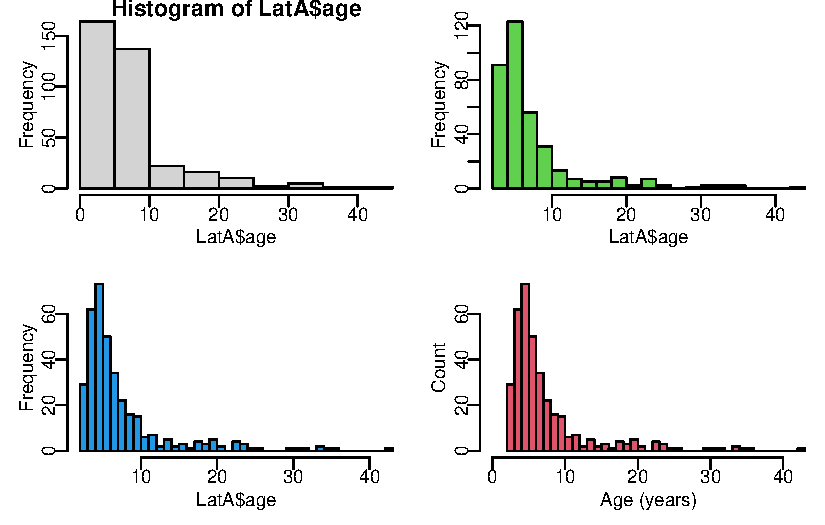
\includegraphics[keepaspectratio]{02-NonIntroductiontoR_files/figure-latex/unnamed-chunk-6-1.pdf}}
\caption{\label{fig:unnamed-chunk-6}An example series of histograms using data from the MQMF data set LatA, illustrating how one can iterate towards a final plot. See also the function uphist().}
\end{figure}

\subsection{因素处理}\label{ux56e0ux7d20ux5904ux7406}

R的一个可能导致挫折和困难的方面是使用因素来表示分类变量。这将分类变量转换为因子的级别(不同值),甚至是已经有数值的因子。例如,在标准化渔业CPUE时,通常至少使用一些分类变量,因此,如果一个水深类别为50 - 600米,每个步骤为50,那么在标准化中需要将这些类别作为固定的分类因子而不是数值处理。但是,一旦转换为一组因子,它们就不再表现为原始的数值变量,而这通常是绘制时所需要的。但是,如果它们最初是\emph{数值}的,则可以使用函数\texttt{facttonum()}进行恢复。在探索与因素有关的一些问题的示例代码中,请注意\texttt{try()}函数的使用(另请参阅\texttt{tryCatch()})。这用于防止r-code由于试图将一个因子乘以标量的错误而停止。这在开发代码和使用bookdown和Rmarkdown编写书籍时非常有用。

\begin{Shaded}
\begin{Highlighting}[]
 \CommentTok{\#Dealing with factors/categories can be tricky  }
\NormalTok{DepCat }\OtherTok{\textless{}{-}} \FunctionTok{as.factor}\NormalTok{(}\FunctionTok{rep}\NormalTok{(}\FunctionTok{seq}\NormalTok{(}\DecValTok{300}\NormalTok{,}\DecValTok{600}\NormalTok{,}\DecValTok{50}\NormalTok{),}\DecValTok{2}\NormalTok{)); DepCat  }
\end{Highlighting}
\end{Shaded}

\begin{verbatim}
##  [1] 300 350 400 450 500 550 600 300 350 400 450 500 550 600
## Levels: 300 350 400 450 500 550 600
\end{verbatim}

\begin{Shaded}
\begin{Highlighting}[]
\FunctionTok{try}\NormalTok{(}\DecValTok{5} \SpecialCharTok{*}\NormalTok{ DepCat[}\DecValTok{3}\NormalTok{], }\AttributeTok{silent=}\ConstantTok{FALSE}\NormalTok{) }\CommentTok{\#only returns NA and a warning!  }
\end{Highlighting}
\end{Shaded}

\begin{verbatim}
## Warning in Ops.factor(5, DepCat[3]): '*' not meaningful for factors
\end{verbatim}

\begin{verbatim}
## [1] NA
\end{verbatim}

\begin{Shaded}
\begin{Highlighting}[]
\FunctionTok{as.numeric}\NormalTok{(DepCat) }\CommentTok{\# returns the levels not the original values  }
\end{Highlighting}
\end{Shaded}

\begin{verbatim}
##  [1] 1 2 3 4 5 6 7 1 2 3 4 5 6 7
\end{verbatim}

\begin{Shaded}
\begin{Highlighting}[]
\FunctionTok{as.numeric}\NormalTok{(}\FunctionTok{levels}\NormalTok{(DepCat)) }\CommentTok{\#converts 7 levels not the replicates  }
\end{Highlighting}
\end{Shaded}

\begin{verbatim}
## [1] 300 350 400 450 500 550 600
\end{verbatim}

\begin{Shaded}
\begin{Highlighting}[]
\NormalTok{DepCat }\OtherTok{\textless{}{-}} \FunctionTok{as.numeric}\NormalTok{(}\FunctionTok{levels}\NormalTok{(DepCat))[DepCat] }\CommentTok{\# try ?facttonum  }
 \CommentTok{\#converts replicates in DepCat to numbers, not just the levels   }
\DecValTok{5} \SpecialCharTok{*}\NormalTok{ DepCat[}\DecValTok{3}\NormalTok{]   }\CommentTok{\# now treat DepCat as numeric  }
\end{Highlighting}
\end{Shaded}

\begin{verbatim}
## [1] 2000
\end{verbatim}

\begin{Shaded}
\begin{Highlighting}[]
\NormalTok{DepCat }\OtherTok{\textless{}{-}} \FunctionTok{as.factor}\NormalTok{(}\FunctionTok{rep}\NormalTok{(}\FunctionTok{seq}\NormalTok{(}\DecValTok{300}\NormalTok{,}\DecValTok{600}\NormalTok{,}\DecValTok{50}\NormalTok{),}\DecValTok{2}\NormalTok{)); DepCat  }
\end{Highlighting}
\end{Shaded}

\begin{verbatim}
##  [1] 300 350 400 450 500 550 600 300 350 400 450 500 550 600
## Levels: 300 350 400 450 500 550 600
\end{verbatim}

\begin{Shaded}
\begin{Highlighting}[]
\FunctionTok{facttonum}\NormalTok{(DepCat)  }
\end{Highlighting}
\end{Shaded}

\begin{verbatim}
##  [1] 300 350 400 450 500 550 600 300 350 400 450 500 550 600
\end{verbatim}

通常,获取data.frame的一个副本并在该副本中分解变量会更简单,因此,如果您想使用原始变量进行进一步的操作或绘图,您不需要将它们从数字转换为因子。

当数据被读入R中的data.frame时,默认的行为是将字符串或字符视为因子。您可以通过在控制台中输入\texttt{options()}来发现很多R选项的默认设置。如果你搜索\$stringsAsFactors(注意大写字母),你会发现它默认为TRUE。如果您希望关闭此功能,可以使用\texttt{option(stringsAsFactors=FALSE)}轻松完成。从关于因素的代码块中可以明显看出,在处理分类变量时需要格外小心。

\subsection{数据输入}\label{ux6570ux636eux8f93ux5165}

与所有编程语言(和统计包)一样,一个共同的需求是输入数据以便进行分析。R非常擅长数据操作,这类事情在Crawley(2007)等书中有很好的描述。当然,也有许多处理数据操作的R包。一个特别有用的是\texttt{dplr},它是\texttt{tidyverse}组的一部分。但是在这里,我们只会提到几种将数据输入r的方法。一种非常常见和低级的方法是简单地使用文本文件作为输入。我仍然经常使用逗号分隔值(.csv)文件,因为它易于生成,而且可以从许多不同的编辑器打开和编辑。可以轻松使用\texttt{read.csv()}或\texttt{read.table()}。一旦数据被读入R,就可以通过\texttt{save(object,file="filename.RData")}将其保存为更有效的存储格式,之后可以使用\texttt{load(file="filename.RData")}将其加载到R。查看\texttt{?save}和\texttt{?load}的细节。

在本书的示例中,我们将使用属于MQMF包一部分的数据集,但是通过复制这些数据集中使用的格式,一旦将数据加载到R中,您就可以使用自己的数据了。

\section{编写函数}\label{ux7f16ux5199ux51fdux6570}

如果你打算使用R来进行任何分析,你通常会使用一个文本编辑器来输入你的R代码,并且至少保存这些脚本以备以后使用。在许多情况下,您可能需要重复一系列命令,这些命令可能使用的变量和或参数的输入值有所不同。尽管使用\texttt{source()}作为中间步骤并非不可能,但这种情况和许多其他情况最好的解决办法是将代码转换为函数。您将在下面的文本和MQMF包中看到许多函数示例,为了充分利用文本中表达的思想,您会发现学习如何编写自己的函数很有帮助。

函数的结构总是相同的:

\begin{Shaded}
\begin{Highlighting}[]
 \CommentTok{\#Outline of a function\textquotesingle{}s structure  }
\NormalTok{functionname }\OtherTok{\textless{}{-}} \ControlFlowTok{function}\NormalTok{(argument1, fun,...) \{  }
  \CommentTok{\# body of the function   }
  \CommentTok{\#   }
  \CommentTok{\# the input arguments and body of a function can include other  }
  \CommentTok{\# functions, which may have their own arguments, which is what  }
  \CommentTok{\# the ... is for. One can include other inputs that are used but  }
  \CommentTok{\# not defined early on and may depend on what function is brought  }
  \CommentTok{\# into the main function. See for example negLL(), and others   }
\NormalTok{  answer }\OtherTok{\textless{}{-}} \FunctionTok{fun}\NormalTok{(argument1) }\SpecialCharTok{+} \DecValTok{2}   
  \FunctionTok{return}\NormalTok{(answer)  }
\NormalTok{\} }\CommentTok{\# end of functionname  }
\FunctionTok{functionname}\NormalTok{(}\FunctionTok{c}\NormalTok{(}\DecValTok{1}\NormalTok{,}\DecValTok{2}\NormalTok{,}\DecValTok{3}\NormalTok{,}\DecValTok{4}\NormalTok{,}\DecValTok{5}\NormalTok{),mean)  }\CommentTok{\# = mean(1,2,3,4,5)= 3 + 2 = 5  }
\end{Highlighting}
\end{Shaded}

\begin{verbatim}
## [1] 5
\end{verbatim}

我们将开发一个示例来说明如何将这些函数组合在一起。

\subsection{简单函数}\label{ux7b80ux5355ux51fdux6570}

通常我们会有一个简单的公式,比如生长函数或者描述鱼类成熟度的函数。例如,von Bertalanffy曲线在渔业研究中使用得相当多。

\begin{equation}
\hat{L_t}=L_{\infty}{\left (1-e^{-K(t-t_0)} \right )}  
\label{eq:lab1}
\end{equation}

在R中这个\eqref{eq:lab1}式可以以多种方式呈现,第一个简单的代码在一个代码块中,用年龄步长进行循环运算,或者矢量化,或者更合理,使用方程转化为一个函数,可以多次调用而不是复制显式行代码。

\begin{Shaded}
\begin{Highlighting}[]
 \CommentTok{\# Implement the von Bertalanffy curve in multiple ways  }
\NormalTok{ages }\OtherTok{\textless{}{-}} \DecValTok{1}\SpecialCharTok{:}\DecValTok{20}  
\NormalTok{nages }\OtherTok{\textless{}{-}} \FunctionTok{length}\NormalTok{(ages)  }
\NormalTok{Linf }\OtherTok{\textless{}{-}} \DecValTok{50}\NormalTok{;  K }\OtherTok{\textless{}{-}} \FloatTok{0.2}\NormalTok{;  t0 }\OtherTok{\textless{}{-}} \SpecialCharTok{{-}}\FloatTok{0.75}  
 \CommentTok{\# first try a for loop to calculate length for each age  }
\NormalTok{loopLt }\OtherTok{\textless{}{-}} \FunctionTok{numeric}\NormalTok{(nages)  }
\ControlFlowTok{for}\NormalTok{ (ag }\ControlFlowTok{in}\NormalTok{ ages) loopLt[ag] }\OtherTok{\textless{}{-}}\NormalTok{ Linf }\SpecialCharTok{*}\NormalTok{ (}\DecValTok{1} \SpecialCharTok{{-}} \FunctionTok{exp}\NormalTok{(}\SpecialCharTok{{-}}\NormalTok{K }\SpecialCharTok{*}\NormalTok{ (ag }\SpecialCharTok{{-}}\NormalTok{ t0)))  }
 \CommentTok{\# the equations are automatically vectorized so more efficient  }
\NormalTok{vecLt }\OtherTok{\textless{}{-}}\NormalTok{ Linf }\SpecialCharTok{*}\NormalTok{ (}\DecValTok{1} \SpecialCharTok{{-}} \FunctionTok{exp}\NormalTok{(}\SpecialCharTok{{-}}\NormalTok{K }\SpecialCharTok{*}\NormalTok{ (ages }\SpecialCharTok{{-}}\NormalTok{ t0))) }\CommentTok{\# or we can convert   }
 \CommentTok{\# the equation into a function and use it again and again  }
\NormalTok{vB }\OtherTok{\textless{}{-}} \ControlFlowTok{function}\NormalTok{(pars,inages) \{ }\CommentTok{\# requires pars=c(Linf,K,t0)  }
  \FunctionTok{return}\NormalTok{(pars[}\DecValTok{1}\NormalTok{] }\SpecialCharTok{*}\NormalTok{ (}\DecValTok{1} \SpecialCharTok{{-}} \FunctionTok{exp}\NormalTok{(}\SpecialCharTok{{-}}\NormalTok{pars[}\DecValTok{2}\NormalTok{] }\SpecialCharTok{*}\NormalTok{ (inages }\SpecialCharTok{{-}}\NormalTok{ pars[}\DecValTok{3}\NormalTok{]))))  }
\NormalTok{\}  }
\NormalTok{funLt }\OtherTok{\textless{}{-}} \FunctionTok{vB}\NormalTok{(}\FunctionTok{c}\NormalTok{(Linf,K,t0),ages)  }
\NormalTok{ans }\OtherTok{\textless{}{-}} \FunctionTok{cbind}\NormalTok{(ages,funLt,vecLt,loopLt)  }
\end{Highlighting}
\end{Shaded}

\begin{longtable}[]{@{}rrrr@{}}
\caption{\label{tab:table1}Three different ways of generating the same growth curve}\tabularnewline
\toprule\noalign{}
ages & funLt & vecLt & loopLt \\
\midrule\noalign{}
\endfirsthead
\toprule\noalign{}
ages & funLt & vecLt & loopLt \\
\midrule\noalign{}
\endhead
\bottomrule\noalign{}
\endlastfoot
1 & 14.77 & 14.77 & 14.77 \\
2 & 21.15 & 21.15 & 21.15 \\
3 & 26.38 & 26.38 & 26.38 \\
4 & 30.66 & 30.66 & 30.66 \\
5 & 34.17 & 34.17 & 34.17 \\
6 & 37.04 & 37.04 & 37.04 \\
7 & 39.39 & 39.39 & 39.39 \\
8 & 41.31 & 41.31 & 41.31 \\
9 & 42.89 & 42.89 & 42.89 \\
10 & 44.18 & 44.18 & 44.18 \\
11 & 45.23 & 45.23 & 45.23 \\
12 & 46.10 & 46.10 & 46.10 \\
13 & 46.80 & 46.80 & 46.80 \\
14 & 47.38 & 47.38 & 47.38 \\
15 & 47.86 & 47.86 & 47.86 \\
16 & 48.25 & 48.25 & 48.25 \\
17 & 48.56 & 48.56 & 48.56 \\
18 & 48.82 & 48.82 & 48.82 \\
19 & 49.04 & 49.04 & 49.04 \\
20 & 49.21 & 49.21 & 49.21 \\
\end{longtable}

使用向量化比使用循环更有效地编写代码,而且一旦人们习惯了这种想法,代码也会变得更易读。当然,可以直接复制进行计算的R的矢量化行,即\texttt{vecLt\ \textless{}-\ Linf\ *\ (1\ -\ exp(-\ k\ *\ (ages\ -\ t0)))},而不是使用函数调用。但也可以在函数中包含错误检查和其他细节,使用函数调用应该有助于避免意外引入错误。此外,许多函数包含大量的代码行,因此使用函数调用也使整个程序更易于阅读和维护。

\begin{Shaded}
\begin{Highlighting}[]
 \CommentTok{\#A vB function with some error checking  }
\NormalTok{vB }\OtherTok{\textless{}{-}} \ControlFlowTok{function}\NormalTok{(pars,inages) \{ }\CommentTok{\# requires pars=c(Linf,K,t0)  }
  \ControlFlowTok{if}\NormalTok{ (}\FunctionTok{is.numeric}\NormalTok{(pars) }\SpecialCharTok{\&} \FunctionTok{is.numeric}\NormalTok{(inages)) \{  }
\NormalTok{    Lt }\OtherTok{\textless{}{-}}\NormalTok{ pars[}\DecValTok{1}\NormalTok{] }\SpecialCharTok{*}\NormalTok{ (}\DecValTok{1} \SpecialCharTok{{-}} \FunctionTok{exp}\NormalTok{(}\SpecialCharTok{{-}}\NormalTok{pars[}\DecValTok{2}\NormalTok{] }\SpecialCharTok{*}\NormalTok{ (inages }\SpecialCharTok{{-}}\NormalTok{ pars[}\DecValTok{3}\NormalTok{])))  }
\NormalTok{  \} }\ControlFlowTok{else}\NormalTok{ \{ }\FunctionTok{stop}\NormalTok{(}\FunctionTok{cat}\NormalTok{(}\StringTok{"Not all input values are numeric! }\SpecialCharTok{\textbackslash{}n}\StringTok{"}\NormalTok{)) \}  }
  \FunctionTok{return}\NormalTok{(Lt)  }
\NormalTok{\}  }
\NormalTok{param }\OtherTok{\textless{}{-}} \FunctionTok{c}\NormalTok{(}\DecValTok{50}\NormalTok{, }\FloatTok{0.2}\NormalTok{,}\StringTok{"{-}0.75"}\NormalTok{)  }
\NormalTok{funLt }\OtherTok{\textless{}{-}} \FunctionTok{vB}\NormalTok{(}\FunctionTok{as.numeric}\NormalTok{(param),ages) }\CommentTok{\#try without the as.numeric  }
\FunctionTok{halftable}\NormalTok{(}\FunctionTok{cbind}\NormalTok{(ages,funLt))  }
\end{Highlighting}
\end{Shaded}

\begin{verbatim}
##    ages    funLt ages    funLt
## 1     1 14.76560   11 45.23154
## 2     2 21.15251   12 46.09592
## 3     3 26.38167   13 46.80361
## 4     4 30.66295   14 47.38301
## 5     5 34.16816   15 47.85739
## 6     6 37.03799   16 48.24578
## 7     7 39.38760   17 48.56377
## 8     8 41.31130   18 48.82411
## 9     9 42.88630   19 49.03726
## 10   10 44.17579   20 49.21178
\end{verbatim}

\subsection{函数输入值}\label{ux51fdux6570ux8f93ux5165ux503c}

使用函数有很多优点。每个函数都有自己的分析环境,其主要优点是每个函数的环境都与函数外部的分析隔离开来。此外,全局环境(在其中完成许多工作)与不同函数中的工作是隔离的。因此,在函数中可以声明一个变量\emph{popnum},并以多种方式更改它的值,但这对函数外同名的变量没有影响。这意味着一个函数的操作范围仅限于该函数。有一些方法可以让函数内部发生的事情直接影响外部变量,但我不会教人们坏习惯,我只会给出搜索符号的提示-\textgreater\textgreater。忘记特殊的情况,一个函数与它发现自己所在的环境(一个人可以有函数,在函数中,在函数中,\ldots)交互的唯一方式是通过它的参数,以及通过它完成时的返回。在上面定义的\texttt{vB()}函数中,参数是\emph{pars} 和 \emph{inages},它显式地返回\emph{Lt}。函数将返回上一次活动计算的结果,但在本书中,我们总是调用\texttt{return()}以确保返回的内容是显式和清晰的。有时,人们可以牺牲增加的简洁来增加清晰度。

在使用函数时,可以显式地使用参数名\texttt{vB(pars=param,\ inages=1:20)}或隐式地使用\texttt{vB(param,1:20)}。如果隐式使用,则输入参数的顺序很重要。如果以错误的顺序输入,函数将愉快地使用1:20的前三个值作为参数,并将param=c(50,0.02, 0.75)作为所需的年龄(从\emph{VB(ages, param)}获得以下预测长度:1.0000 -269.4264 -1807.0424)。如果使用了参数名,那么顺序并不重要。输入所有这些名称可能会让人觉得需要付出更多的努力,但它最终确实使编程变得更容易,并且充当了另一个自我文档的来源。当然,应该开发一种适合自己的编程风格,自然地,可以从错误中学习。

从本质上讲,软件是顺从的。如果我们将\texttt{vB()}函数的参数前后混乱,如我们所见,它仍然会尽力返回一个答案或尝试失败。使用相对简单的软件和函数,不难确保任何这样的参数和数据输入以正确的顺序和可识别的形式呈现给函数。一旦我们开始生成更多的相互联系和复杂的软件,其中一个过程的输出形成了对其他过程的输入,那么所涉及的计划需要扩展到参数和数据使用的格式。错误检查就变得比只使用单个函数重要得多。

\subsection{R对象}\label{rux5bf9ux8c61}

我们将R语言视为一种编程语言,在编写任何软件时都应该认真对待它的设计。只关注R,有两个原则可以帮助这样的设计(Chambers, 2016, p4)。 1. 存在于R中的一切都是一个对象。

\begin{enumerate}
\def\labelenumi{\arabic{enumi}.}
\setcounter{enumi}{1}
\tightlist
\item
  在R中发生的一切都是一个函数调用。
\end{enumerate}

这意味着任何函数输入的每个参数或形参和数据集都是R对象,就像函数(如果有的话)返回的都是R对象一样。

\subsection{对象范围}\label{ux5bf9ux8c61ux8303ux56f4}

您可能想知道为什么我在上面的\texttt{vB()}函数参数中使用\emph{inages}而不是\emph{ages}。这纯粹是为了避免混淆每个变量的范围。如上所述,在R中,所有操作都发生在环境中,全局环境是在使用控制台或简单脚本时输入的环境。重要的是要认识到,您编写的任何函数都有自己的环境,其中包含内部变量的作用域。然而,即使R对象没有作为参数传递给函数,该对象仍然可以在函数中看到。但是,函数内部的工作对全局或调用环境是隐藏的。如果在函数内部定义了一个变量,但在函数外部使用了相同的变量名,那么当使用变量名时,它首先会在自己的环境中搜索,并使用内部定义的版本,而不是外部定义的版本。不过,最好的做法是在函数内部使用与函数外部不同的对象名称。

\begin{Shaded}
\begin{Highlighting}[]
 \CommentTok{\# demonstration that the globel environment is \textquotesingle{}visible\textquotesingle{} inside a  }
 \CommentTok{\# a function it calls, but the function\textquotesingle{}s environment remains  }
 \CommentTok{\# invisible to the global or calling environment  }
\NormalTok{vBscope }\OtherTok{\textless{}{-}} \ControlFlowTok{function}\NormalTok{(pars) \{ }\CommentTok{\# requires pars=c(Linf,K,t0)  }
\NormalTok{  rhside }\OtherTok{\textless{}{-}}\NormalTok{ (}\DecValTok{1} \SpecialCharTok{{-}} \FunctionTok{exp}\NormalTok{(}\SpecialCharTok{{-}}\NormalTok{pars[}\DecValTok{2}\NormalTok{] }\SpecialCharTok{*}\NormalTok{ (ages }\SpecialCharTok{{-}}\NormalTok{ pars[}\DecValTok{3}\NormalTok{])))  }
\NormalTok{  Lt }\OtherTok{\textless{}{-}}\NormalTok{ pars[}\DecValTok{1}\NormalTok{] }\SpecialCharTok{*}\NormalTok{ rhside  }
  \FunctionTok{return}\NormalTok{(Lt)  }
\NormalTok{\}  }
\NormalTok{ages }\OtherTok{\textless{}{-}} \DecValTok{1}\SpecialCharTok{:}\DecValTok{10}\NormalTok{; param }\OtherTok{\textless{}{-}} \FunctionTok{c}\NormalTok{(}\DecValTok{50}\NormalTok{,}\FloatTok{0.2}\NormalTok{,}\SpecialCharTok{{-}}\FloatTok{0.75}\NormalTok{)  }
\FunctionTok{vBscope}\NormalTok{(param)  }
\end{Highlighting}
\end{Shaded}

\begin{verbatim}
##  [1] 14.76560 21.15251 26.38167 30.66295 34.16816 37.03799 39.38760
##  [8] 41.31130 42.88630 44.17579
\end{verbatim}

\begin{Shaded}
\begin{Highlighting}[]
\FunctionTok{try}\NormalTok{(rhside)    }\CommentTok{\# note the use of try() which can trap errors ?try  }
\end{Highlighting}
\end{Shaded}

\begin{verbatim}
## Error in eval(expr, envir) : object 'rhside' not found
\end{verbatim}

\subsection{函数输入与输出}\label{ux51fdux6570ux8f93ux5165ux4e0eux8f93ux51fa}

像大多数软件一样,R函数总是有输入和输出(尽管两者可能都是\emph{NULL};函数的括号可以为空,例如\texttt{parsyn()})。当输入参数向量或数据矩阵时,采用标准格式是明智的,我的意思是设置标准格式。这样,任何处理此类数据的函数都可以对其格式进行假设。理想情况下,在使用任何输入数据之前进行数据检查仍然是一个好主意,但这可以通过遵循任何确定的标准格式来简化。

重要的是要知道和理解输入到每个函数中的数据的结构,因为向量繁殖需要以不同的方式引用到矩阵中,而矩阵的行为也与data.frame不同。通常最好通过列名显式地引用矩阵,因为不能保证所有这样的数据集都按照\emph{schaef}中找到的顺序。我们可以比较\texttt{schaef{[},2{]}}和\texttt{schaef{[},"catch"{]}},和\texttt{schaef\$catch}。

\begin{Shaded}
\begin{Highlighting}[]
 \CommentTok{\#Bring the data{-}set schaef into the working of global environment  }
\FunctionTok{data}\NormalTok{(schaef)  }
\end{Highlighting}
\end{Shaded}

\begin{Shaded}
\begin{Highlighting}[]
 \CommentTok{\#examine the properties of the data{-}set schaef  }
\FunctionTok{class}\NormalTok{(schaef)  }
\end{Highlighting}
\end{Shaded}

\begin{verbatim}
## [1] "data.frame"
\end{verbatim}

\begin{Shaded}
\begin{Highlighting}[]
\NormalTok{a }\OtherTok{\textless{}{-}}\NormalTok{ schaef[}\DecValTok{1}\SpecialCharTok{:}\DecValTok{5}\NormalTok{,}\DecValTok{2}\NormalTok{]  }
\NormalTok{b }\OtherTok{\textless{}{-}}\NormalTok{ schaef[}\DecValTok{1}\SpecialCharTok{:}\DecValTok{5}\NormalTok{,}\StringTok{"catch"}\NormalTok{]  }
\NormalTok{c }\OtherTok{\textless{}{-}}\NormalTok{ schaef}\SpecialCharTok{$}\NormalTok{catch[}\DecValTok{1}\SpecialCharTok{:}\DecValTok{5}\NormalTok{]  }
\FunctionTok{cbind}\NormalTok{(a,b,c)  }
\end{Highlighting}
\end{Shaded}

\begin{verbatim}
##          a     b     c
## [1,] 60913 60913 60913
## [2,] 72294 72294 72294
## [3,] 78353 78353 78353
## [4,] 91522 91522 91522
## [5,] 78288 78288 78288
\end{verbatim}

\begin{Shaded}
\begin{Highlighting}[]
\NormalTok{mschaef }\OtherTok{\textless{}{-}} \FunctionTok{as.matrix}\NormalTok{(schaef)  }
\NormalTok{mschaef[}\DecValTok{1}\SpecialCharTok{:}\DecValTok{5}\NormalTok{,}\StringTok{"catch"}\NormalTok{]  }\CommentTok{\# ok  }
\end{Highlighting}
\end{Shaded}

\begin{verbatim}
##  1934  1935  1936  1937  1938 
## 60913 72294 78353 91522 78288
\end{verbatim}

\begin{Shaded}
\begin{Highlighting}[]
\NormalTok{d }\OtherTok{\textless{}{-}} \FunctionTok{try}\NormalTok{(mschaef}\SpecialCharTok{$}\NormalTok{catch[}\DecValTok{1}\SpecialCharTok{:}\DecValTok{5}\NormalTok{]) }\CommentTok{\#invalid for matrices  }
\end{Highlighting}
\end{Shaded}

\begin{verbatim}
## Error in mschaef$catch : $ operator is invalid for atomic vectors
\end{verbatim}

\begin{Shaded}
\begin{Highlighting}[]
\NormalTok{d  }\CommentTok{\# had we not used try()eveerything would have stopped.  }
\end{Highlighting}
\end{Shaded}

\begin{verbatim}
## [1] "Error in mschaef$catch : $ operator is invalid for atomic vectors\n"
## attr(,"class")
## [1] "try-error"
## attr(,"condition")
## <simpleError in mschaef$catch: $ operator is invalid for atomic vectors>
\end{verbatim}

通过测试\texttt{schaef}对象的\emph{类},我们可以看到它是data.frame而不是矩阵。因此,处理这些输入可能不像乍一看那么简单。是的,列的顺序可能会改变,但名称也可能不同。因此,我们至少要做一些检查,使我们的软件至少在一定程度上是安全的。通常我们是唯一使用我们编写的软件的人,但我发现这并不意味着我不需要尝试使它万无一失(似乎有时我是愚蠢的)。

注意,在\texttt{schaef}中,我们使用了所有小写的列标题,这并不总是常见的。正如我们所看到的,列名很重要,因为引用data.frame通常会更好,就像引用矩阵一样。通常,在编程时,我们可以使用不止一个选项。我们可以强制输入数据矩阵变成data.frame,但也可以强制列名为小写。我知道列名已经是小写的了,但是这里我们讨论的是一个接收任意给定数据集的函数。

\begin{Shaded}
\begin{Highlighting}[]
 \CommentTok{\#Convert column names of a data.frame or matrix to lowercase  }
\NormalTok{dolittle }\OtherTok{\textless{}{-}} \ControlFlowTok{function}\NormalTok{(indat) \{  }
\NormalTok{   indat1 }\OtherTok{\textless{}{-}} \FunctionTok{as.data.frame}\NormalTok{(indat)  }
   \FunctionTok{colnames}\NormalTok{(indat) }\OtherTok{\textless{}{-}} \FunctionTok{tolower}\NormalTok{(}\FunctionTok{colnames}\NormalTok{(indat))  }
   \FunctionTok{return}\NormalTok{(}\FunctionTok{list}\NormalTok{(}\AttributeTok{dfdata=}\NormalTok{indat1,}\AttributeTok{indat=}\FunctionTok{as.matrix}\NormalTok{(indat)))  }
\NormalTok{\} }\CommentTok{\# return the original and the new version  }
\FunctionTok{colnames}\NormalTok{(schaef) }\OtherTok{\textless{}{-}} \FunctionTok{toupper}\NormalTok{(}\FunctionTok{colnames}\NormalTok{(schaef))  }
\NormalTok{out }\OtherTok{\textless{}{-}} \FunctionTok{dolittle}\NormalTok{(schaef)  }
\FunctionTok{str}\NormalTok{(out, }\AttributeTok{width=}\DecValTok{63}\NormalTok{, }\AttributeTok{strict.width=}\StringTok{"cut"}\NormalTok{)  }
\end{Highlighting}
\end{Shaded}

\begin{verbatim}
## List of 2
##  $ dfdata:'data.frame':  22 obs. of  4 variables:
##   ..$ YEAR  : int [1:22] 1934 1935 1936 1937 1938 1939 1940 1..
##   ..$ CATCH : int [1:22] 60913 72294 78353 91522 78288 110417..
##   ..$ EFFORT: int [1:22] 5879 6295 6771 8233 6830 10488 10801..
##   ..$ CPUE  : num [1:22] 10.4 11.5 11.6 11.1 11.5 ...
##  $ indat : num [1:22, 1:4] 1934 1935 1936 1937 1938 ...
##   ..- attr(*, "dimnames")=List of 2
##   .. ..$ : chr [1:22] "1934" "1935" "1936" "1937" ...
##   .. ..$ : chr [1:4] "year" "catch" "effort" "cpue"
\end{verbatim}

因此,在接下来的内容中,我们将尝试仅对与渔业相关的数据使用小写列名,我们将使用标准名称''year''、``catch''、``cpue''等,但我们也将在期望输入数据矩阵的函数中包含一条转换为\emph{tolower}的语句。当输入包含与渔业相关的数据矩阵、年龄组成数据、与生长、成熟、补充和选择性有关的生物常数向量以及其他数据的更复杂列表对象时,这些细节就变得更加重要。在任何稍微复杂一点的软件设计中,都应该确定标准格式并检查此类输入。

在\texttt{schaef}的情况下,这是在评估中与剩余产量模型一起使用的数据。这是合理的想法开发函数提前预支了一个先于它是否包含所有所需的数据,在数据是否有差距,和其他细节,之前用于评估一个甚至可以开发\emph{S3}类为特定分析,这将允许将函数添加到通用函数,如\emph{print}、\emph{plot}、\emph{summary},以及创建自己的新泛型方法函数。

另外,可以简单地编写函数来为特定的分析生成可定制的图,以执行可能重复多次的特定任务。可以通过函数\texttt{plotspmdat()}找到一个示例,该函数将获取典型的渔业数据,并绘制渔获量和cpue的时间序列。

\begin{Shaded}
\begin{Highlighting}[]
 \CommentTok{\#Could have used an S3 plot method had we defined a class   Fig.2.2 }
\FunctionTok{plotspmdat}\NormalTok{(schaef) }\CommentTok{\# examine the code as an eg of a custom plot  }
\end{Highlighting}
\end{Shaded}

\begin{figure}
\centering
\pandocbounded{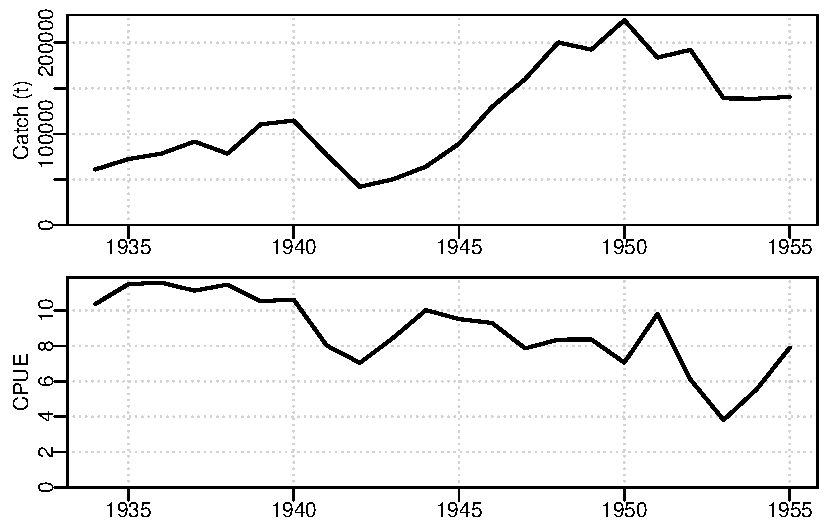
\includegraphics[keepaspectratio]{02-NonIntroductiontoR_files/figure-latex/unnamed-chunk-22-1.pdf}}
\caption{\label{fig:unnamed-chunk-22}The catch and cpue data from the MQMF data-set schaef plotted automatically.}
\end{figure}

\section{附录:少有人使用的函数}\label{ux9644ux5f55ux5c11ux6709ux4ebaux4f7fux7528ux7684ux51fdux6570}

下面列出的函数只是为了帮助读者记住R中一些容易被遗忘的函数,因为它们很少被使用,尽管它们在处理实际问题时非常有用。

\texttt{getNamespaceExports("MQMF")}

\texttt{getS3method("print","default")} 通常 \texttt{print.default} 也可以

\texttt{ls(“package:MQMF”)} 列出包中的输出函数

\texttt{ls.str(“package:MQMF”)}列出函数及其语法

\texttt{methods(“print”)}列出适用的S3方法

\texttt{on.exit(suppressWarnings(sink()))} 退出运行的清洗方法(即使失败)

\texttt{packageDescription("MQMF")}

\texttt{RNGkind()}正在使用的随机数生成器

\texttt{sessionInfo()}

\texttt{sink("filename",split=TRUE)} then after lots of screen output sink(),

\texttt{suppressWarnings(sink())} removes a sink quietly if a run crashes and leaves one open

\section{附录:其它学习资源}\label{ux9644ux5f55ux5176ux5b83ux5b66ux4e60ux8d44ux6e90}

Other Books: these two have a tidyverse bent.

Wickham and Grolemund (2017) \emph{R for Data Science} \url{https://r4ds.had.co.nz/}

Grolemund (2014) \emph{Hands-On Programming with R} \url{https://rstudio-education.github.io/hopr/}

There are blogs devoted to R. I rather like \url{https://www.r-bloggers.com/} but I get that delivered to my email. This blog lists many others.

There is even an open-source journal concerning R

\url{https://journal.r-project.org/}

\chapter{简单种群模型}\label{ux7b80ux5355ux79cdux7fa4ux6a21ux578b}

\section{简介}\label{ux7b80ux4ecb-2}

简单的种群模型构成了众多渔业模型的基础,事实上,渔业模型与生态种群模型的区别只是人为的划分。理解任何种群模型的运行方式都将有助于更好地理解渔业模型,因此在本章中,我们将使用R来检验种群生物学中的一些基本思想的动力学。

\subsection{离散Logistic模型}\label{ux79bbux6563logisticux6a21ux578b}

我们将首先考察已成为生态学中经典种群模型之一的离散逻辑斯蒂模型所展示的动力学。这种模型出现在许多地方,以许多不同的形式出现,因此值得进行一些详细的探索。这里我们将使用Schaefer(1954, 1957)版本,它有四个组成部分或项:

\begin{equation}
\begin{split}  
N_{t=0} &= N_0 \\  
{{N}_{t+1}} &= {{N}_{t}}+{{r}{N}_{t}}\left( 1-{{\left( \frac{{{N}_{t}}}{K} \right)}} \right)-{{C}_{t}}  
\end{split}  
\label{eq:eq31}
\end{equation}

\(N_t\)项为时间\(t\)时的数量(如年\(t\)的开始时),最后一项为\(C_t\),它是在时间\(t\)内(如年份\(t\))捕获的渔获量。第一行反映了初始状态,定义为时间0时的数量(或生物量)。要注意下标,因为无论是数量还是生物量,它们都是指特定时间的数量和生物量,通常是确定的时间段\(t\)的开始时的数量或生物量,而渔获量指的是整个时间段\(t\)内的渔获量。这个方程是对时间步长\(t\)的动力学的总结; 它是一个差分方程而不是连续微分方程。第二个方程的中间项是更复杂的组成部分,该项定义了所谓的渔业生产曲线。它由\(r\) 和\(K\)组成,\(r\)为种群的内在增长率,\(K\)为承载力或最大种群规模。如果动力学表示为在开发开始之前处于平衡状态,那么\(N_0\)会取与\(K\)相同的值,但它是分开的,以考虑任何时间序列开始时偏离均衡的情况。在\textbf{MQMF}的\texttt{discretelogistic()}函数中包含了另外的参数\(p\),将在\emph{剩余产量模型(Surplus Production Models )}一章中详细讨论。这里只说明默认值\(p=1.0\) 就足够了,式\eqref{eq:eq31}中的方程等同于Schaefer模型。这里,Schaefer模型输出实时数量,尽管在渔业中,它通常直接用实时生物量(\(B_t\))表示。这些术语可以以这种方式改变,这一事实强调了该模型忽略了生物学实际和属性,如种群体长结构和年龄结构,以及性别和其他属性之间的差异。令人惊讶的是,这样一个简单的模型在理论和实践中仍然是有用的。

我们可以通过将式\eqref{eq:eq31}的中间项与\(N_t\)值的向量绘制成曲线来说明产量曲线。子项\(rN_t\)表示无限制的种群指数增长,在这个离散形式的方程中,并将此项与\(N_t\)相加。因此,只要\(r>0.1\)及渔获量为0,我们就可以期待从方程的\(N_t+rN_t\)部分得到种群的无尽增长。然而,子项\((1−(N_t/K))\)为抑制指数增长的项,而且随着种群规模的增长,这种作用越来越大。这就是所谓的密度依赖效应。

\begin{Shaded}
\begin{Highlighting}[]
\CommentTok{\#Code to produce Figure 3.1. Note the two one{-}line functions  }
\NormalTok{surprod }\OtherTok{\textless{}{-}} \ControlFlowTok{function}\NormalTok{(Nt,r,K) }\FunctionTok{return}\NormalTok{((r}\SpecialCharTok{*}\NormalTok{Nt)}\SpecialCharTok{*}\NormalTok{(}\DecValTok{1}\SpecialCharTok{{-}}\NormalTok{(Nt}\SpecialCharTok{/}\NormalTok{K)))  }
\NormalTok{densdep }\OtherTok{\textless{}{-}} \ControlFlowTok{function}\NormalTok{(Nt,K) }\FunctionTok{return}\NormalTok{((}\DecValTok{1}\SpecialCharTok{{-}}\NormalTok{(Nt}\SpecialCharTok{/}\NormalTok{K)))  }
\NormalTok{r }\OtherTok{\textless{}{-}} \FloatTok{1.2}\NormalTok{; K }\OtherTok{\textless{}{-}} \FloatTok{1000.0}\NormalTok{; Nt }\OtherTok{\textless{}{-}} \FunctionTok{seq}\NormalTok{(}\DecValTok{10}\NormalTok{,}\DecValTok{1000}\NormalTok{,}\DecValTok{10}\NormalTok{)  }
\FunctionTok{par}\NormalTok{(}\AttributeTok{mfrow=}\FunctionTok{c}\NormalTok{(}\DecValTok{2}\NormalTok{,}\DecValTok{1}\NormalTok{),}\AttributeTok{mai=}\FunctionTok{c}\NormalTok{(}\FloatTok{0.4}\NormalTok{,}\FloatTok{0.4}\NormalTok{,}\FloatTok{0.05}\NormalTok{,}\FloatTok{0.05}\NormalTok{),}\AttributeTok{oma=}\FunctionTok{c}\NormalTok{(}\FloatTok{0.0}\NormalTok{,}\DecValTok{0}\NormalTok{,}\FloatTok{0.0}\NormalTok{,}\FloatTok{0.0}\NormalTok{))   }
\FunctionTok{par}\NormalTok{(}\AttributeTok{cex=}\FloatTok{0.75}\NormalTok{, }\AttributeTok{mgp=}\FunctionTok{c}\NormalTok{(}\FloatTok{1.35}\NormalTok{,}\FloatTok{0.35}\NormalTok{,}\DecValTok{0}\NormalTok{), }\AttributeTok{font.axis=}\DecValTok{7}\NormalTok{,}\AttributeTok{font=}\DecValTok{7}\NormalTok{,}\AttributeTok{font.lab=}\DecValTok{7}\NormalTok{)   }
\FunctionTok{plot1}\NormalTok{(Nt,}\FunctionTok{surprod}\NormalTok{(Nt,r,K),}\AttributeTok{xlab=}\StringTok{"Population Nt"}\NormalTok{,}\AttributeTok{defpar=}\ConstantTok{FALSE}\NormalTok{,  }
      \AttributeTok{ylab=}\StringTok{"Production"}\NormalTok{)  }
\FunctionTok{plot1}\NormalTok{(Nt,}\FunctionTok{densdep}\NormalTok{(Nt,K),}\AttributeTok{xlab=}\StringTok{"Population Nt"}\NormalTok{,}\AttributeTok{defpar=}\ConstantTok{FALSE}\NormalTok{,  }
      \AttributeTok{ylab=}\StringTok{"Density{-}Dependence"}\NormalTok{)  }
\end{Highlighting}
\end{Shaded}

\begin{figure}
\centering
\pandocbounded{\includegraphics[keepaspectratio]{03-simpopmodel_files/figure-latex/fig3-1-1.pdf}}
\caption{\label{fig:fig3-1} The full production curve for the discrete Schaefer (1954, 1957) surplus production model and the equivalent implied linear density dependent relationship with population size.}
\end{figure}

密度依赖是种群规模调节的重要组成部分(May and McLean, 2007)。从图\ref{fig:fig3-1}可以明显看出,Schaefer模型中的密度依赖项与种群规模呈线性递减关系。这就是''线性密度依赖''一词的字面意思,你可以在种群动态文献中找到它。这个密度依赖项,试图补偿由\(rN_t\)驱动的指数增长 ,限制种群规模不大于未捕捞种群规模\(K\)的长期平均(关于补偿不足时会发生什么,请参阅下一节)。

\subsection{动态行为}\label{ux52a8ux6001ux884cux4e3a}

最大种群规模真正限制在\(K\)值时,一般认为Schaefer模型的微分方程形式是非常稳定的。令人惊讶的是,人们发现离散形式的动力学更为复杂和有趣(May, 1973,1976)。我们已经在函数\texttt{discretelogistic()}中实现了上述方程的一种形式,你可以通过\emph{?discrete telogistic}读取它的帮助文件,并且可以通过在控制台输入\texttt{discrete\ telogistic}来查看它的代码(注意,没有括号)。如果您检查这个函数中的代码,您将看到它使用\emph{for}循环来逐年间计算每年的种群规模。我希望,作为一名R程序员,您会想知道为什么我不使用向量化方法来避免使用\emph{for}循环。这突出了种群动力学的一个基本方面,即\(t\)时刻的数量总是\(t-1\)时刻数量的函数(初始条件可能于\(N_0\)参数)。种群动态的顺序性质意味着我们不能以任何有效的方式使用矢量化。种群动态的顺序性是如此明显的事实,以至于它施加在种群模型上的约束和结构常常被忽视。

\texttt{discretelogistic()}函数(不可视地)输出时间\emph{year}(为\(year\))、\(t\)时的数量\(n_t\)(为\(nt\))以及\(t+1\)时的数量\(n_{t+1}\)(为\(nt1\))的矩阵。该矩阵也给出\textbf{MQMF}中包含的了\emph{dynpop}类和S3方法(\emph{plot.dynpop};见\emph{A non-introduction to R} 一章S3类和方法的使用。如果要查看代码,在控制台中办入*MQMF:::plot.dynpop,记住当中是3个'':``,而非2个)。当然,人们可以写任何想写的东西。试着将\texttt{rv}的值 设定为0.5、1.95、2.2、2.475、2.56和2.8,用这些值按顺序运行下面的代码。

\begin{Shaded}
\begin{Highlighting}[]
 \CommentTok{\#Code for Figure 3.2. Try varying the value of rv from 0.5{-}2.8  }
\NormalTok{yrs }\OtherTok{\textless{}{-}} \DecValTok{100}\NormalTok{; rv}\OtherTok{=}\FloatTok{2.8}\NormalTok{;  Kv }\OtherTok{\textless{}{-}} \FloatTok{1000.0}\NormalTok{; Nz}\OtherTok{=}\DecValTok{100}\NormalTok{; catch}\OtherTok{=}\FloatTok{0.0}\NormalTok{; p}\OtherTok{=}\FloatTok{1.0}  
\NormalTok{ans }\OtherTok{\textless{}{-}} \FunctionTok{discretelogistic}\NormalTok{(}\AttributeTok{r=}\NormalTok{rv,}\AttributeTok{K=}\NormalTok{Kv,}\AttributeTok{N0=}\NormalTok{Nz,}\AttributeTok{Ct=}\NormalTok{catch,}\AttributeTok{Yrs=}\NormalTok{yrs,}\AttributeTok{p=}\NormalTok{p)  }
\NormalTok{avcatch }\OtherTok{\textless{}{-}} \FunctionTok{mean}\NormalTok{(ans[(yrs}\DecValTok{{-}50}\NormalTok{)}\SpecialCharTok{:}\NormalTok{yrs,}\StringTok{"nt"}\NormalTok{],}\AttributeTok{na.rm=}\ConstantTok{TRUE}\NormalTok{) }\CommentTok{\#used in text  }
\NormalTok{label }\OtherTok{\textless{}{-}} \FunctionTok{paste0}\NormalTok{(}\StringTok{"r="}\NormalTok{,rv,}\StringTok{" K="}\NormalTok{,Kv,}\StringTok{" Ct="}\NormalTok{,catch, }\StringTok{" N0="}\NormalTok{,Nz,}\StringTok{" p="}\NormalTok{,}\AttributeTok{p=}\NormalTok{p)  }
\FunctionTok{plot}\NormalTok{(ans, }\AttributeTok{main=}\NormalTok{label, }\AttributeTok{cex=}\FloatTok{0.9}\NormalTok{, }\AttributeTok{font=}\DecValTok{7}\NormalTok{) }\CommentTok{\#Schaefer dynamics  }
\end{Highlighting}
\end{Shaded}

\begin{figure}
\centering
\pandocbounded{\includegraphics[keepaspectratio]{03-simpopmodel_files/figure-latex/fig3-2-1.pdf}}
\caption{\label{fig:fig3-2}Schaefer model dynamics. The left plot is the numbers by year, illustrating chaotic dynamics from an r-value of 2.8. The right plot is numbers-at-time t+1 against time t, known as a phase plot. The final 20\% of points are in red to illustrate any equilibrium behaviour. The grey diagonal is the 1:1 line.}
\end{figure}

如果你运行导致图\ref{fig:fig3-2}的代码,使用上面提到的6个\texttt{rv}值,你应该会看到一个单调阻尼平衡(一个实心点),然后是一个阻尼振荡平衡(仍然是一个实心点),然后是介于阻尼振荡平衡和两环稳定极限环之间的东西(有点涂抹了两个实心点)。当\(r = 2.475\)时,有一个4圈稳定的极限环(4个实心点),当\(r = 2.56\)时,有一个8圈稳定的极限环。最后,当\(r = 2.8\)时,动态以混乱告终,尽管所有的点都落在如图所示的抛物线上,但每一步的结果都不是随机的,也不是直接可预测的。在混沌理论中,这个抛物线被称为奇怪的吸引子,尽管这是一个非常简单的吸引子。这种混沌系统也依赖于起始条件。如果把初始数字改为101而不是100,数字的时间线就会发生根本性的变化,尽管抛物线保持不变。当然,我们可以输入任意范围的数字,也可以使用稍微不同的模型来改变动态。虽然混乱很有趣,玩起来也很有趣(Gleick,1988;Lauwerier, 1991),但在模拟自然种群的实际应用中似乎很少有用。事实上,一些人声称,他们观察到的明显的随机性是由种群对随机环境效应的反应引起的,而不是由密度依赖模型中的补偿不足和补偿过度引入的非线性(Higgins等,1997)。

在实践中,如果发现一个模型引起了明显的混乱或循环行为,甚至是负的种群数量,尝试确定所观察到的是真实的生物群体行为(显然不是负数),或者更简单地说,只是一个特殊参数的数学表达式。人们总是可以通过在计算中包含诸如\(max((B_t+(rB_t)(1-(B_t/K))-C_t),0)\)之类以避免模型向下跌落到0以下(参见\texttt{discretelogistic()}代码。类似地,用\(min((B_t+(rB_t)(1-(B_t/K))-C_t),1.1K)\)以避免计算值高于\(K\)),尽管对代码的此类添加仍然是临时的(应该,比如,任何超过\(K\)的值都应允许,是\(1.1K\),还是\(1.0K\)?有些种群自然变动的)。在\emph{剩余产量模型(Surplus Production Models)} 一章中我们将研究罚函数的使用,罚函数可用于防止在估计这些参数时产生异常值,同时避免使用钝工具,如\(max(\cdots,0)\)。

我们可以通过将\texttt{discretelogistic()}函数的不可见输出转换为可以使用的对象来检查每年的实际种群规模,如表(3.1)所示。

\begin{Shaded}
\begin{Highlighting}[]
\CommentTok{\#run discrete logistic dynamics for 600 years  }
\NormalTok{yrs}\OtherTok{=}\DecValTok{600}  
\NormalTok{ans }\OtherTok{\textless{}{-}} \FunctionTok{discretelogistic}\NormalTok{(}\AttributeTok{r=}\FloatTok{2.55}\NormalTok{,}\AttributeTok{K=}\FloatTok{1000.0}\NormalTok{,}\AttributeTok{N0=}\DecValTok{100}\NormalTok{,}\AttributeTok{Ct=}\FloatTok{0.0}\NormalTok{,}\AttributeTok{Yrs=}\NormalTok{yrs)  }
\NormalTok{ans[}\DecValTok{571}\SpecialCharTok{:}\DecValTok{600}\NormalTok{,]}
\end{Highlighting}
\end{Shaded}

\begin{verbatim}
##     year        nt       nt1
## 571  571  493.9379 1131.3442
## 572  572 1131.3442  752.4257
## 573  573  752.4257 1227.4429
## 574  574 1227.4429  515.5513
## 575  575  515.5513 1152.4346
## 576  576 1152.4346  704.4738
## 577  577  704.4738 1235.3595
## 578  578 1235.3595  493.9379
## 579  579  493.9379 1131.3442
## 580  580 1131.3442  752.4257
## 581  581  752.4257 1227.4429
## 582  582 1227.4429  515.5513
## 583  583  515.5513 1152.4346
## 584  584 1152.4346  704.4738
## 585  585  704.4738 1235.3595
## 586  586 1235.3595  493.9379
## 587  587  493.9379 1131.3442
## 588  588 1131.3442  752.4257
## 589  589  752.4257 1227.4429
## 590  590 1227.4429  515.5513
## 591  591  515.5513 1152.4346
## 592  592 1152.4346  704.4738
## 593  593  704.4738 1235.3595
## 594  594 1235.3595  493.9379
## 595  595  493.9379 1131.3442
## 596  596 1131.3442  752.4257
## 597  597  752.4257 1227.4429
## 598  598 1227.4429  515.5513
## 599  599  515.5513 1152.4346
## 600  600 1152.4346  704.4738
\end{verbatim}

当我们设置\(r\)值来产生2循环的稳定极限(例如\(r=2.2\)),可以从其他年份的数字重复中清楚地看到。检查实际的数字显然比相信情节的视觉印象更准确。这也意味着我们可以尽可能详细地询问结果。在上述情况下,最近50年的平均渔获量为859.675,明显小于1000的\(K\)值。由于\(N_{t+1}\)与\(N_t\)的相位关系,上一年的最后一行通常不会有\(N_{t+1}\)的值,因此,在代码中,输入的年份数增加1,以便最终生成\(N_{t+1}\)(请参阅代码)。

\subsection{发现行为间的界限}\label{ux53d1ux73b0ux884cux4e3aux95f4ux7684ux754cux9650}

我们可以通过求ans中\(nt\)和\(Nt1\)列的行平均值来找到一个稳定的极限环,检查最后100个值(四舍五入到小数点后三位)。\texttt{table()}函数的名称标识循环点的值(如果有的话)。如果只有一个或两个平均值来确定一个渐近平衡或一个两周期稳定的极限环。通过检查每个ans对象中值的时间序列,可以搜索所标识值的第一次出现,从而确定循环行为(到小数点后三位)何时第一次出现。我们将这些值四舍五入,并使用600年或更长的时间,因为如果我们使用所有15位小数,任何超过8的周期都可能无法被清楚地识别出来(尝试将r = 2.63更改为5;试着用\texttt{plot(ans)})。

\begin{Shaded}
\begin{Highlighting}[]
 \CommentTok{\#run discretelogistic and search for repeated values of Nt  }
\NormalTok{yrs }\OtherTok{\textless{}{-}} \DecValTok{600}  
\NormalTok{ans }\OtherTok{\textless{}{-}} \FunctionTok{discretelogistic}\NormalTok{(}\AttributeTok{r=}\FloatTok{2.55}\NormalTok{,}\AttributeTok{K=}\FloatTok{1000.0}\NormalTok{,}\AttributeTok{N0=}\DecValTok{100}\NormalTok{,}\AttributeTok{Ct=}\FloatTok{0.0}\NormalTok{,}\AttributeTok{Yrs=}\NormalTok{yrs)  }
\NormalTok{avt }\OtherTok{\textless{}{-}} \FunctionTok{round}\NormalTok{(}\FunctionTok{apply}\NormalTok{(ans[(yrs}\DecValTok{{-}100}\NormalTok{)}\SpecialCharTok{:}\NormalTok{(yrs}\DecValTok{{-}1}\NormalTok{),}\DecValTok{2}\SpecialCharTok{:}\DecValTok{3}\NormalTok{],}\DecValTok{1}\NormalTok{,mean),}\DecValTok{2}\NormalTok{)  }
\NormalTok{count }\OtherTok{\textless{}{-}} \FunctionTok{table}\NormalTok{(avt)  }
\NormalTok{count[count }\SpecialCharTok{\textgreater{}} \DecValTok{1}\NormalTok{] }\CommentTok{\# with r=2.55 you should find an 8{-}cycle limit  }
\end{Highlighting}
\end{Shaded}

\begin{verbatim}
## avt
## 812.64 833.99 864.65  871.5 928.45 941.88 969.92 989.93 
##     12     13     12     13     12     13     12     13
\end{verbatim}

我们可以建立一个程序来寻找\(r\)的值 生成不同周期的稳定极限环,尽管下面的代码只是部分成功。通过设置一个\emph{for}循环,将不同的值替换为\(r\) 值输入到\texttt{discretelogistic()},我们可以搜索一个长时间序列的最后几年在数字的时间序列中唯一的值。然而,舍入误差可能会导致意想不到的结果,特别是在不同类型的动态行为之间的边界。我们可以通过将检查的数字四舍五入到小数点后三位来避免这些问题,但请尝试在下面的代码中散列该行,以查看问题变得更糟。

\begin{Shaded}
\begin{Highlighting}[]
\CommentTok{\#searches for unique solutions given an r value  see Table 3.2}
\NormalTok{testseq }\OtherTok{\textless{}{-}} \FunctionTok{seq}\NormalTok{(}\FloatTok{1.9}\NormalTok{,}\FloatTok{2.59}\NormalTok{,}\FloatTok{0.01}\NormalTok{)  }
\NormalTok{nseq }\OtherTok{\textless{}{-}} \FunctionTok{length}\NormalTok{(testseq)  }
\NormalTok{result }\OtherTok{\textless{}{-}} \FunctionTok{matrix}\NormalTok{(}\DecValTok{0}\NormalTok{,}\AttributeTok{nrow=}\NormalTok{nseq,}\AttributeTok{ncol=}\DecValTok{2}\NormalTok{,  }
                 \AttributeTok{dimnames=}\FunctionTok{list}\NormalTok{(testseq,}\FunctionTok{c}\NormalTok{(}\StringTok{"r"}\NormalTok{,}\StringTok{"Unique"}\NormalTok{)))  }
\NormalTok{yrs }\OtherTok{\textless{}{-}} \DecValTok{600}  
\ControlFlowTok{for}\NormalTok{ (i }\ControlFlowTok{in} \DecValTok{1}\SpecialCharTok{:}\NormalTok{nseq) \{  }\CommentTok{\# i = 31  }
\NormalTok{   rval }\OtherTok{\textless{}{-}}\NormalTok{ testseq[i]  }
\NormalTok{   ans }\OtherTok{\textless{}{-}} \FunctionTok{discretelogistic}\NormalTok{(}\AttributeTok{r=}\NormalTok{rval,}\AttributeTok{K=}\FloatTok{1000.0}\NormalTok{,}\AttributeTok{N0=}\DecValTok{100}\NormalTok{,}\AttributeTok{Ct=}\FloatTok{0.0}\NormalTok{,}\AttributeTok{Yrs=}\NormalTok{yrs)  }
\NormalTok{   ans }\OtherTok{\textless{}{-}}\NormalTok{ ans[}\SpecialCharTok{{-}}\NormalTok{yrs,] }\CommentTok{\# remove last year, see str(ans) for why  }
\NormalTok{   ans[,}\StringTok{"nt1"}\NormalTok{] }\OtherTok{\textless{}{-}} \FunctionTok{round}\NormalTok{(ans[,}\StringTok{"nt1"}\NormalTok{],}\DecValTok{3}\NormalTok{) }\CommentTok{\#try hashing this out  }
\NormalTok{   result[i,] }\OtherTok{\textless{}{-}} \FunctionTok{c}\NormalTok{(rval,}\FunctionTok{length}\NormalTok{(}\FunctionTok{unique}\NormalTok{(}\FunctionTok{tail}\NormalTok{(ans[,}\StringTok{"nt1"}\NormalTok{],}\DecValTok{100}\NormalTok{))))  }
\NormalTok{\}  }
\end{Highlighting}
\end{Shaded}

在上面的例子中,有一个\(r\)值的范围,在最近的100次观测中,\(r\)值的最大值为60。这些代表了计算机上舍入错误的问题。如果持续的年数急剧增加,那么预期最终会出现一种平衡。无论哪种情况,都有一个明显的分裂或过渡,从单一平衡点,到2循环,到4循环,最后到8循环稳定极限。在行为的每个开关上,由于舍入误差,结果有一些不稳定性。

\subsection{经典的混沌分岔图}\label{ux7ecfux5178ux7684ux6df7ux6c8cux5206ux5c94ux56fe}

May(1976)对基于差分方程的单物种种群模型的动力学进行了综述。在这本书中,他从非常简单的模型描述了混沌动力学的潜力。在那篇文章中,他绘制了一个图,他称之为分岔图,它显示了模型的平衡属性如何随着单个参数的改变而改变。我们可以使用\texttt{discretelogistic()}函数和下面的代码,以几乎任何精度复制图\ref{fig:fig3-3}。

在分叉图的混乱中,偶尔会有一些简化,用在图的墨水空间中的白色空白来表示。可以通过替换\emph{testseq}向量中的值检查其中的一些位置;如下限值=2.82,上限= 2.87;和inc = 0.0001。这些起始点提供了更多的细节,在这些细节中有以前被掩盖的细节。这些起始点提供了更多的细节,在这些细节中有以前被掩盖的细节。这些也可以检查通过改变数值\emph{testseq \textless{} - c(2.845, 2.855, 0.00001)},于是分岔,2 - 4 -和更高的周期可以看到(甚至可以看到更多的细节通过改变\emph{limy= 0}参数绑定y-轴在\(limy=c(600, 750)\)内感兴趣的区域绑定y轴所需的范围。这个图是通过在每个r的序列值处使用最终尾\textless- 100点绘制的。可以增加模拟的年数和绘制的最终点的数量,以获得更好的分辨率在混沌区域。要查看更多细节,请在需要细节的区域扩展规模。

\begin{Shaded}
\begin{Highlighting}[]
 \CommentTok{\#the R code for the bifurcation function  }
\NormalTok{bifurcation }\OtherTok{\textless{}{-}} \ControlFlowTok{function}\NormalTok{(testseq,}\AttributeTok{taill=}\DecValTok{100}\NormalTok{,}\AttributeTok{yrs=}\DecValTok{1000}\NormalTok{,}\AttributeTok{limy=}\DecValTok{0}\NormalTok{,}\AttributeTok{incx=}\FloatTok{0.001}\NormalTok{)\{  }
\NormalTok{  nseq }\OtherTok{\textless{}{-}} \FunctionTok{length}\NormalTok{(testseq)  }
\NormalTok{  result }\OtherTok{\textless{}{-}} \FunctionTok{matrix}\NormalTok{(}\DecValTok{0}\NormalTok{,}\AttributeTok{nrow=}\NormalTok{nseq,}\AttributeTok{ncol=}\DecValTok{2}\NormalTok{,  }
                  \AttributeTok{dimnames=}\FunctionTok{list}\NormalTok{(testseq,}\FunctionTok{c}\NormalTok{(}\StringTok{"r"}\NormalTok{,}\StringTok{"Unique Values"}\NormalTok{)))  }
\NormalTok{  result2 }\OtherTok{\textless{}{-}} \FunctionTok{matrix}\NormalTok{(}\ConstantTok{NA}\NormalTok{,}\AttributeTok{nrow=}\NormalTok{nseq,}\AttributeTok{ncol=}\NormalTok{taill)  }
  \ControlFlowTok{for}\NormalTok{ (i }\ControlFlowTok{in} \DecValTok{1}\SpecialCharTok{:}\NormalTok{nseq) \{    }
\NormalTok{     rval }\OtherTok{\textless{}{-}}\NormalTok{ testseq[i]  }
\NormalTok{     ans }\OtherTok{\textless{}{-}} \FunctionTok{discretelogistic}\NormalTok{(}\AttributeTok{r=}\NormalTok{rval,}\AttributeTok{K=}\FloatTok{1000.0}\NormalTok{,}\AttributeTok{N0=}\DecValTok{100}\NormalTok{,}\AttributeTok{Ct=}\FloatTok{0.0}\NormalTok{,}\AttributeTok{Yrs=}\NormalTok{yrs)  }
\NormalTok{     ans[,}\StringTok{"nt1"}\NormalTok{] }\OtherTok{\textless{}{-}} \FunctionTok{round}\NormalTok{(ans[,}\StringTok{"nt1"}\NormalTok{],}\DecValTok{4}\NormalTok{)  }
\NormalTok{     result[i,] }\OtherTok{\textless{}{-}} \FunctionTok{c}\NormalTok{(rval,}\FunctionTok{length}\NormalTok{(}\FunctionTok{unique}\NormalTok{(}\FunctionTok{tail}\NormalTok{(ans[,}\StringTok{"nt1"}\NormalTok{],taill))))  }
\NormalTok{     result2[i,] }\OtherTok{\textless{}{-}} \FunctionTok{tail}\NormalTok{(ans[,}\StringTok{"nt1"}\NormalTok{],taill)  }
\NormalTok{  \}    }
  \ControlFlowTok{if}\NormalTok{ (limy[}\DecValTok{1}\NormalTok{] }\SpecialCharTok{==} \DecValTok{0}\NormalTok{) limy }\OtherTok{\textless{}{-}} \FunctionTok{c}\NormalTok{(}\DecValTok{0}\NormalTok{,}\FunctionTok{getmax}\NormalTok{(result2,}\AttributeTok{mult=}\FloatTok{1.02}\NormalTok{))  }
  \FunctionTok{parset}\NormalTok{() }\CommentTok{\# plot taill values against taill of each r value  }
  \FunctionTok{plot}\NormalTok{(}\FunctionTok{rep}\NormalTok{(testseq[}\DecValTok{1}\NormalTok{],taill),result2[}\DecValTok{1}\NormalTok{,],}\AttributeTok{type=}\StringTok{"p"}\NormalTok{,}\AttributeTok{pch=}\DecValTok{16}\NormalTok{,}\AttributeTok{cex=}\FloatTok{0.1}\NormalTok{,  }
   \AttributeTok{ylim=}\NormalTok{limy,}\AttributeTok{xlim=}\FunctionTok{c}\NormalTok{(}\FunctionTok{min}\NormalTok{(testseq)}\SpecialCharTok{*}\NormalTok{(}\DecValTok{1}\SpecialCharTok{{-}}\NormalTok{incx),}\FunctionTok{max}\NormalTok{(testseq)}\SpecialCharTok{*}\NormalTok{(}\DecValTok{1}\SpecialCharTok{+}\NormalTok{incx)),  }
    \AttributeTok{xlab=}\StringTok{"r value"}\NormalTok{,}\AttributeTok{yaxs=}\StringTok{"i"}\NormalTok{,}\AttributeTok{xaxs=}\StringTok{"i"}\NormalTok{,}\AttributeTok{ylab=}\StringTok{"Equilibrium Numbers"}\NormalTok{,  }
     \AttributeTok{panel.first=}\FunctionTok{grid}\NormalTok{())  }
  \ControlFlowTok{for}\NormalTok{ (i }\ControlFlowTok{in} \DecValTok{2}\SpecialCharTok{:}\NormalTok{nseq)  }
      \FunctionTok{points}\NormalTok{(}\FunctionTok{rep}\NormalTok{(testseq[i],taill),result2[i,],}\AttributeTok{pch=}\DecValTok{16}\NormalTok{,}\AttributeTok{cex=}\FloatTok{0.1}\NormalTok{)  }
  \FunctionTok{return}\NormalTok{(}\FunctionTok{invisible}\NormalTok{(}\FunctionTok{list}\NormalTok{(}\AttributeTok{result=}\NormalTok{result,}\AttributeTok{result2=}\NormalTok{result2)))  }
\NormalTok{\} }\CommentTok{\# end of bifurcation  }
\end{Highlighting}
\end{Shaded}

\begin{Shaded}
\begin{Highlighting}[]
 \CommentTok{\#Alternative r value arrangements for you to try; Fig 3.3  }
 \CommentTok{\#testseq \textless{}{-} seq(2.847,2.855,0.00001) \#hash/unhash as needed  }
 \CommentTok{\#bifurcation(testseq,limy=c(600,740),incx=0.0001) \# t  }
 \CommentTok{\#testseq \textless{}{-} seq(2.6225,2.6375,0.00001) \# then explore   }
 \CommentTok{\#bifurcation(testseq,limy=c(660,730),incx=0.0001)   }
\NormalTok{testseq }\OtherTok{\textless{}{-}} \FunctionTok{seq}\NormalTok{(}\FloatTok{1.9}\NormalTok{,}\FloatTok{2.975}\NormalTok{,}\FloatTok{0.0005}\NormalTok{) }\CommentTok{\# modify to explore  }
\FunctionTok{bifurcation}\NormalTok{(testseq,}\AttributeTok{limy=}\DecValTok{0}\NormalTok{)    }
\end{Highlighting}
\end{Shaded}

\begin{figure}
\centering
\pandocbounded{\includegraphics[keepaspectratio]{03-simpopmodel_files/figure-latex/fig3-3-1.pdf}}
\caption{\label{fig:fig3-3}Schaefer model dynamics. A classical bifurcation diagram (May, 1976) plotting equilibrium dynamics against values of r, illustrating the transition from 2-, 4-, 8-cycle, and beyond, including chaotic behaviour.}
\end{figure}

\subsection{捕捞对动态的影响}\label{ux6355ux635eux5bf9ux52a8ux6001ux7684ux5f71ux54cd}

如果我们设置一个默认的\texttt{discretelogisitic()}运行,以在渔获量为零时拥有8个周期的稳定极限,我们可以应用不同水平的恒定渔获量,看看这可能如何影响动态。在这里,我们应用了0,50,200和325个个体(尽管\(N_t\),\(K\)和\(C_t\) 也可能是吨)。当然是初始值\(N_0\)必须大于捕获值,否则可以自由更改值。在下面四种情况中,我们假设\(p\) 值为1.0 (= Schaefer模型)时,可以尝试\(p=1e−08\)探讨使用与Fox模型等价的方法所产生的差异。

\begin{Shaded}
\begin{Highlighting}[]
 \CommentTok{\#Effect of catches on stability properties of discretelogistic  }
\NormalTok{yrs}\OtherTok{=}\DecValTok{50}\NormalTok{; Kval}\OtherTok{=}\FloatTok{1000.0}  
\NormalTok{nocatch }\OtherTok{\textless{}{-}} \FunctionTok{discretelogistic}\NormalTok{(}\AttributeTok{r=}\FloatTok{2.56}\NormalTok{,}\AttributeTok{K=}\NormalTok{Kval,}\AttributeTok{N0=}\DecValTok{500}\NormalTok{,}\AttributeTok{Ct=}\DecValTok{0}\NormalTok{,}\AttributeTok{Yrs=}\NormalTok{yrs)  }
\NormalTok{catch50 }\OtherTok{\textless{}{-}} \FunctionTok{discretelogistic}\NormalTok{(}\AttributeTok{r=}\FloatTok{2.56}\NormalTok{,}\AttributeTok{K=}\NormalTok{Kval,}\AttributeTok{N0=}\DecValTok{500}\NormalTok{,}\AttributeTok{Ct=}\DecValTok{50}\NormalTok{,}\AttributeTok{Yrs=}\NormalTok{yrs)  }
\NormalTok{catch200 }\OtherTok{\textless{}{-}} \FunctionTok{discretelogistic}\NormalTok{(}\AttributeTok{r=}\FloatTok{2.56}\NormalTok{,}\AttributeTok{K=}\NormalTok{Kval,}\AttributeTok{N0=}\DecValTok{500}\NormalTok{,}\AttributeTok{Ct=}\DecValTok{200}\NormalTok{,}\AttributeTok{Yrs=}\NormalTok{yrs)  }
\NormalTok{catch300 }\OtherTok{\textless{}{-}} \FunctionTok{discretelogistic}\NormalTok{(}\AttributeTok{r=}\FloatTok{2.56}\NormalTok{,}\AttributeTok{K=}\NormalTok{Kval,}\AttributeTok{N0=}\DecValTok{500}\NormalTok{,}\AttributeTok{Ct=}\DecValTok{300}\NormalTok{,}\AttributeTok{Yrs=}\NormalTok{yrs)  }
\end{Highlighting}
\end{Shaded}

我们组合了一个小函数\texttt{plottime()},以简化最终对象的重复绘图。我们还使用了效用函数\texttt{parsyn()}来辅助\texttt{par()}函数的语法,以定义基本图形图的边界。请注意,生成这样的函数可以简化后续的代码,我建议构建这样一个有用的函数集合,可以与函数\texttt{source()}一起使用,将它们引入到自己的会话中(就像预包;不要忘记在编写函数时记录文档,RStudio甚至有一个插入Roxygen骨架命令)。在这里,随着捕获量的增加,可以看到动态开始稳定4到2周期,然后渐近平衡。注意,随着渔获量的增加,随着时间的推移(图表底部的数字),平均渔获量下降。

\begin{Shaded}
\begin{Highlighting}[]
 \CommentTok{\#Effect of different catches on n{-}cyclic behaviour Fig3.4  }
\NormalTok{plottime }\OtherTok{\textless{}{-}} \ControlFlowTok{function}\NormalTok{(x,ylab) \{  }
\NormalTok{   yrs }\OtherTok{\textless{}{-}} \FunctionTok{nrow}\NormalTok{(x)  }
   \FunctionTok{plot1}\NormalTok{(x[,}\StringTok{"year"}\NormalTok{],x[,}\StringTok{"nt"}\NormalTok{],}\AttributeTok{ylab=}\NormalTok{ylab,}\AttributeTok{defpar=}\ConstantTok{FALSE}\NormalTok{)  }
\NormalTok{   avB }\OtherTok{\textless{}{-}} \FunctionTok{round}\NormalTok{(}\FunctionTok{mean}\NormalTok{(x[(yrs}\DecValTok{{-}40}\NormalTok{)}\SpecialCharTok{:}\NormalTok{yrs,}\StringTok{"nt"}\NormalTok{],}\AttributeTok{na.rm=}\ConstantTok{TRUE}\NormalTok{),}\DecValTok{3}\NormalTok{)  }
   \FunctionTok{mtext}\NormalTok{(avB,}\AttributeTok{side=}\DecValTok{1}\NormalTok{,}\AttributeTok{outer=}\NormalTok{F,}\AttributeTok{line=}\SpecialCharTok{{-}}\FloatTok{1.1}\NormalTok{,}\AttributeTok{font=}\DecValTok{7}\NormalTok{,}\AttributeTok{cex=}\FloatTok{1.0}\NormalTok{)   }
\NormalTok{\} }\CommentTok{\# end of plottime  }
 \CommentTok{\#the oma argument is used to adjust the space around the graph  }
\FunctionTok{par}\NormalTok{(}\AttributeTok{mfrow=}\FunctionTok{c}\NormalTok{(}\DecValTok{2}\NormalTok{,}\DecValTok{2}\NormalTok{),}\AttributeTok{mai=}\FunctionTok{c}\NormalTok{(}\FloatTok{0.25}\NormalTok{,}\FloatTok{0.4}\NormalTok{,}\FloatTok{0.05}\NormalTok{,}\FloatTok{0.05}\NormalTok{),}\AttributeTok{oma=}\FunctionTok{c}\NormalTok{(}\FloatTok{1.0}\NormalTok{,}\DecValTok{0}\NormalTok{,}\FloatTok{0.25}\NormalTok{,}\DecValTok{0}\NormalTok{))   }
\FunctionTok{par}\NormalTok{(}\AttributeTok{cex=}\FloatTok{0.75}\NormalTok{, }\AttributeTok{mgp=}\FunctionTok{c}\NormalTok{(}\FloatTok{1.35}\NormalTok{,}\FloatTok{0.35}\NormalTok{,}\DecValTok{0}\NormalTok{), }\AttributeTok{font.axis=}\DecValTok{7}\NormalTok{,}\AttributeTok{font=}\DecValTok{7}\NormalTok{,}\AttributeTok{font.lab=}\DecValTok{7}\NormalTok{)    }
\FunctionTok{plottime}\NormalTok{(nocatch,}\StringTok{"Catch = 0"}\NormalTok{)  }
\FunctionTok{plottime}\NormalTok{(catch50,}\StringTok{"Catch = 50"}\NormalTok{)  }
\FunctionTok{plottime}\NormalTok{(catch200,}\StringTok{"Catch = 200"}\NormalTok{)  }
\FunctionTok{plottime}\NormalTok{(catch300,}\StringTok{"Catch = 300"}\NormalTok{)  }
\FunctionTok{mtext}\NormalTok{(}\StringTok{"years"}\NormalTok{,}\AttributeTok{side=}\DecValTok{1}\NormalTok{,}\AttributeTok{outer=}\ConstantTok{TRUE}\NormalTok{,}\AttributeTok{line=}\SpecialCharTok{{-}}\FloatTok{0.2}\NormalTok{,}\AttributeTok{font=}\DecValTok{7}\NormalTok{,}\AttributeTok{cex=}\FloatTok{1.0}\NormalTok{)   }
\end{Highlighting}
\end{Shaded}

\begin{figure}
\centering
\pandocbounded{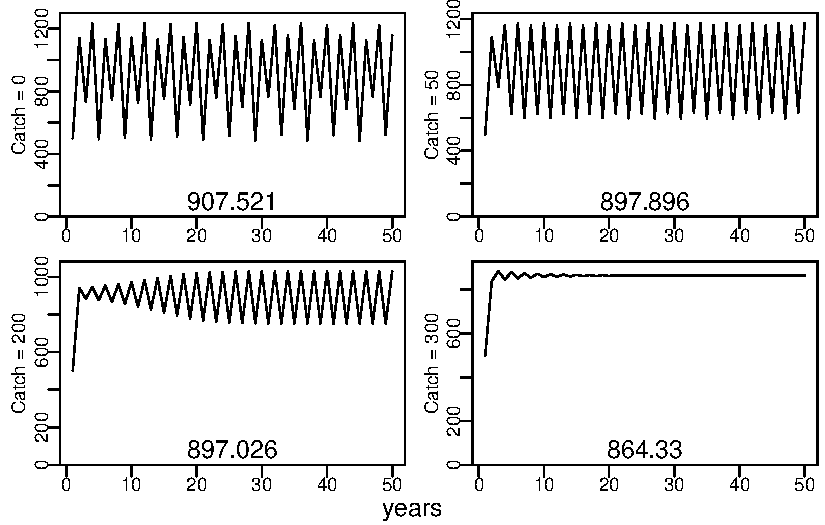
\includegraphics[keepaspectratio]{03-simpopmodel_files/figure-latex/fig3-4-1.pdf}}
\caption{\label{fig:fig3-4}Schaefer model dynamics. The top-left plot depicts the expected unfished dynamics (8-cycle) while the next three plots, with decreasing average catches, illustrate the impact of the increased catches with no other factor changing.}
\end{figure}

我们可以对四个相图做一些类似的事情。这里,我们从\texttt{MQMF:::plot.dynpop()}函数中借用了部分代码,以定义一个小型定制函数,以方便一起绘制四个阶段的图。

\begin{Shaded}
\begin{Highlighting}[]
\CommentTok{\#Phase plot for Schaefer model Fig 3.5  }
\NormalTok{plotphase }\OtherTok{\textless{}{-}} \ControlFlowTok{function}\NormalTok{(x,label,}\AttributeTok{ymax=}\DecValTok{0}\NormalTok{) \{ }\CommentTok{\#x from discretelogistic  }
\NormalTok{  yrs }\OtherTok{\textless{}{-}} \FunctionTok{nrow}\NormalTok{(x)  }
  \FunctionTok{colnames}\NormalTok{(x) }\OtherTok{\textless{}{-}} \FunctionTok{tolower}\NormalTok{(}\FunctionTok{colnames}\NormalTok{(x))  }
  \ControlFlowTok{if}\NormalTok{ (ymax[}\DecValTok{1}\NormalTok{] }\SpecialCharTok{==} \DecValTok{0}\NormalTok{) ymax }\OtherTok{\textless{}{-}} \FunctionTok{getmax}\NormalTok{(x[,}\FunctionTok{c}\NormalTok{(}\DecValTok{2}\SpecialCharTok{:}\DecValTok{3}\NormalTok{)])  }
  \FunctionTok{plot}\NormalTok{(x[,}\StringTok{"nt"}\NormalTok{],x[,}\StringTok{"nt1"}\NormalTok{],}\AttributeTok{type=}\StringTok{"p"}\NormalTok{,}\AttributeTok{pch=}\DecValTok{16}\NormalTok{,}\AttributeTok{cex=}\FloatTok{1.0}\NormalTok{,}\AttributeTok{ylim=}\FunctionTok{c}\NormalTok{(}\DecValTok{0}\NormalTok{,ymax),  }
       \AttributeTok{yaxs=}\StringTok{"i"}\NormalTok{,}\AttributeTok{xlim=}\FunctionTok{c}\NormalTok{(}\DecValTok{0}\NormalTok{,ymax),}\AttributeTok{xaxs=}\StringTok{"i"}\NormalTok{,}\AttributeTok{ylab=}\StringTok{"nt1"}\NormalTok{,}\AttributeTok{xlab=}\StringTok{""}\NormalTok{,  }
       \AttributeTok{panel.first=}\FunctionTok{grid}\NormalTok{(),}\AttributeTok{col=}\StringTok{"darkgrey"}\NormalTok{)  }
\NormalTok{  begin }\OtherTok{\textless{}{-}} \FunctionTok{trunc}\NormalTok{(yrs }\SpecialCharTok{*} \FloatTok{0.6}\NormalTok{) }\CommentTok{\#last 40\% of yrs = 20, when yrs=50  }
  \FunctionTok{points}\NormalTok{(x[begin}\SpecialCharTok{:}\NormalTok{yrs,}\StringTok{"nt"}\NormalTok{],x[begin}\SpecialCharTok{:}\NormalTok{yrs,}\StringTok{"nt1"}\NormalTok{],}\AttributeTok{pch=}\DecValTok{18}\NormalTok{,}\AttributeTok{col=}\DecValTok{1}\NormalTok{,}\AttributeTok{cex=}\FloatTok{1.2}\NormalTok{)  }
  \FunctionTok{mtext}\NormalTok{(label,}\AttributeTok{side=}\DecValTok{1}\NormalTok{,}\AttributeTok{outer=}\NormalTok{F,}\AttributeTok{line=}\SpecialCharTok{{-}}\FloatTok{1.1}\NormalTok{,}\AttributeTok{font=}\DecValTok{7}\NormalTok{,}\AttributeTok{cex=}\FloatTok{1.2}\NormalTok{)   }
\NormalTok{\} }\CommentTok{\# end of plotphase  }
\FunctionTok{par}\NormalTok{(}\AttributeTok{mfrow=}\FunctionTok{c}\NormalTok{(}\DecValTok{2}\NormalTok{,}\DecValTok{2}\NormalTok{),}\AttributeTok{mai=}\FunctionTok{c}\NormalTok{(}\FloatTok{0.25}\NormalTok{,}\FloatTok{0.25}\NormalTok{,}\FloatTok{0.05}\NormalTok{,}\FloatTok{0.05}\NormalTok{),}\AttributeTok{oma=}\FunctionTok{c}\NormalTok{(}\FloatTok{1.0}\NormalTok{,}\FloatTok{1.0}\NormalTok{,}\DecValTok{0}\NormalTok{,}\DecValTok{0}\NormalTok{))   }
\FunctionTok{par}\NormalTok{(}\AttributeTok{cex=}\FloatTok{0.75}\NormalTok{, }\AttributeTok{mgp=}\FunctionTok{c}\NormalTok{(}\FloatTok{1.35}\NormalTok{,}\FloatTok{0.35}\NormalTok{,}\DecValTok{0}\NormalTok{), }\AttributeTok{font.axis=}\DecValTok{7}\NormalTok{,}\AttributeTok{font=}\DecValTok{7}\NormalTok{,}\AttributeTok{font.lab=}\DecValTok{7}\NormalTok{)    }
\FunctionTok{plotphase}\NormalTok{(nocatch,}\StringTok{"Catch = 0"}\NormalTok{,}\AttributeTok{ymax=}\DecValTok{1300}\NormalTok{)  }
\FunctionTok{plotphase}\NormalTok{(catch50,}\StringTok{"Catch = 50"}\NormalTok{,}\AttributeTok{ymax=}\DecValTok{1300}\NormalTok{)  }
\FunctionTok{plotphase}\NormalTok{(catch200,}\StringTok{"Catch = 200"}\NormalTok{,}\AttributeTok{ymax=}\DecValTok{1300}\NormalTok{)  }
\FunctionTok{plotphase}\NormalTok{(catch300,}\StringTok{"Catch = 300"}\NormalTok{,}\AttributeTok{ymax=}\DecValTok{1300}\NormalTok{)  }
\FunctionTok{mtext}\NormalTok{(}\StringTok{"nt"}\NormalTok{,}\AttributeTok{side=}\DecValTok{1}\NormalTok{,}\AttributeTok{outer=}\NormalTok{T,}\AttributeTok{line=}\FloatTok{0.0}\NormalTok{,}\AttributeTok{font=}\DecValTok{7}\NormalTok{,}\AttributeTok{cex=}\FloatTok{1.0}\NormalTok{)  }
\FunctionTok{mtext}\NormalTok{(}\StringTok{"nt+1"}\NormalTok{,}\AttributeTok{side=}\DecValTok{2}\NormalTok{,}\AttributeTok{outer=}\NormalTok{T,}\AttributeTok{line=}\FloatTok{0.0}\NormalTok{,}\AttributeTok{font=}\DecValTok{7}\NormalTok{,}\AttributeTok{cex=}\FloatTok{1.0}\NormalTok{)  }
\end{Highlighting}
\end{Shaded}

\begin{figure}
\centering
\pandocbounded{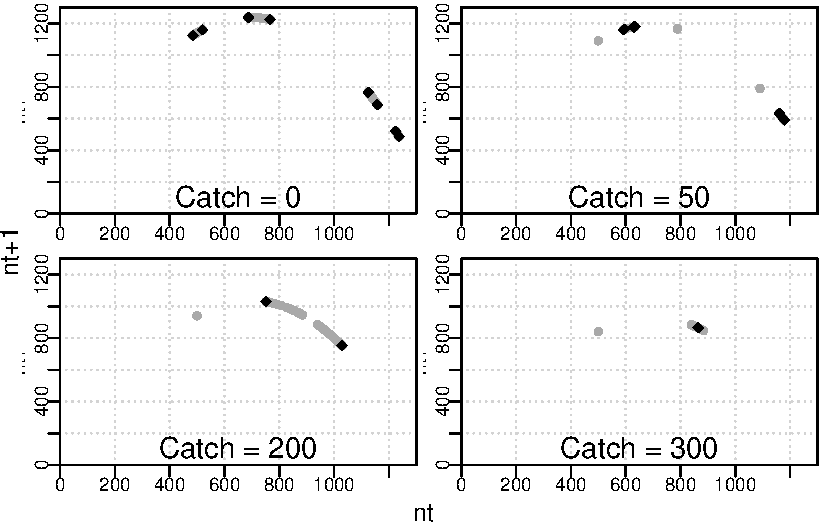
\includegraphics[keepaspectratio]{03-simpopmodel_files/figure-latex/fig3-5-1.pdf}}
\caption{\label{fig:fig3-5}Schaefer model dynamics. Phase plots for each of the four constant catch scenarios}
\end{figure}

随着固定捕获量的增加,隐含抛物线曲线(奇异吸引子)的最大值下降。渔获量(\(\equiv\) 捕食者)似乎对种群的动态有稳定的影响。在自然界中是否如此,将取决于特定种群的生物学是否反映了用于描述动态的模型的基本假设(例如,Schaefer模型假设种群中存在线性密度依赖)。

现在,我们应该很清楚,即使是简单的模型也可以表现出复杂的行为。我们只是稍微触及了这个主题,但同样清楚的是,使用R,可以探索这些想法到任何深度。

\subsection{决定论}\label{ux51b3ux5b9aux8bba}

本章所有的模型都表现出确定性动力学,即使是混沌动力学,在初始条件重复的情况下也会遵循相同的轨迹。当然,在自然界中,这种确定性行为是罕见的。模型总是对可能发生的事情进行抽象。与生产力相关的自然过程(自然死亡率、生长和繁殖)都将随着时间的推移而变化,这是对食物供应、生态相互作用和环境影响(如温度)的响应。通过包括所谓的过程误差,可以将过程中的这种可变性近似地包括到模型中,过程误差可以用方程形式表示为:

\begin{equation}  
{N_{t+1}}={N_t}+{({r+\varepsilon_t}){N_t}}\left( 1-{{\left( \frac{N_t}{(K+\epsilon_t)} \right)}} \right)  
\label{eq:eq32} 
\end{equation}

其中\(\varepsilon\) 和\(\epsilon\) 表示每个模型参数随时间\(t\)变化的正态随机误差。有时,在模拟中,只有一个参数会添加变化。作为种群现象,这将导致种群数量遵循不一定是平滑的轨迹,而且在模拟中,单个复制将不足以捕捉可能的动态的潜在范围。在模拟中是否包括这种过程误差将取决于模拟的目的。在这里,目的是探索确定性种群动态的期望,但应该始终记住,这些模型只是近似,旨在代表平均行为。

\section{年龄结构的建模概念}\label{ux5e74ux9f84ux7ed3ux6784ux7684ux5efaux6a21ux6982ux5ff5}

当然,在我们刚刚考察的剩余产量模型中,最大的简化是,它们忽略了与年龄和个体大小有关的生物学和行为差异的所有方面。这种简化的模型仍然有用(见\emph{剩余产量模型(Surplus Production Models)} 章节),但面对公认的网具选择性(类似于捕食者有偏好的猎物)和不同年龄的生长和繁殖力、渔业和其他自然资源科学家经常在他们的模型中包括年龄和或大小。在这里,我们将只对这些想法进行初步处理,因为在详细讨论这些复杂问题之前,还需要建模动态过程的许多其他细节。

\subsection{世代中的残存}\label{ux4e16ux4ee3ux4e2dux7684ux6b8bux5b58}

很明显,个体的残存,\(S\),两个时间段之间的残存可用\(t+1\)时的数量与\(t\)时的数量的比值表示(记住,如果知道体重与年龄的关系,年龄-数量可以转换为年龄-体质量或年龄-生物量):

\begin{equation}  
S_t=\frac{{{N}_{t+1}}}{{{N}_{t}}}\text{ or }{{N}_{t+1}}={S_t}{N}_{t}  
\label{eq:eq33}
\end{equation}

这种随时间的比例减少暗示着负指数增长。给定瞬时总死亡率为\(Z\) (自然死亡率和捕捞死亡率之和),则每年的残存率(即存活的比例)等于\(e^{−Z}\)。这可以通过设置一个具有恒定初始条件的模拟种群,并应用不同瞬时总死亡率向量来说明。

这将相当于考虑一个单一世代补充的为0+年龄的个体。假设没有移入个体,这样的单一世代种群只能在数量上下降,尽管这看起来很明显,但在考虑年龄结构的种群时,这是重要的直觉。总死亡率(通常用\(Z\)表示)仅仅是自然死亡率(通常用\(M\)表示)和捕捞死亡率(通常用\(F\)表示)的总和。在下面的例子中,请注意,应用\(Z =0.05\) 会导致即使在50年后种群数量也大于零。图示中的每个世代轨迹都描述了种群规模的指数或恒定比例下降。

\begin{Shaded}
\begin{Highlighting}[]
\CommentTok{\#Exponential population declines under different Z. Fig 3.6  }
\NormalTok{yrs }\OtherTok{\textless{}{-}} \DecValTok{50}\NormalTok{;  yrs1 }\OtherTok{\textless{}{-}}\NormalTok{ yrs }\SpecialCharTok{+} \DecValTok{1} \CommentTok{\# to leave room for B[0]  }
\NormalTok{years }\OtherTok{\textless{}{-}} \FunctionTok{seq}\NormalTok{(}\DecValTok{0}\NormalTok{,yrs,}\DecValTok{1}\NormalTok{)  }
\NormalTok{B0 }\OtherTok{\textless{}{-}} \DecValTok{1000}        \CommentTok{\# now alternative total mortality rates  }
\NormalTok{Z }\OtherTok{\textless{}{-}} \FunctionTok{c}\NormalTok{(}\FloatTok{0.05}\NormalTok{,}\FloatTok{0.1}\NormalTok{,}\FloatTok{0.2}\NormalTok{,}\FloatTok{0.4}\NormalTok{,}\FloatTok{0.55}\NormalTok{)   }
\NormalTok{nZ }\OtherTok{\textless{}{-}} \FunctionTok{length}\NormalTok{(Z)  }
\NormalTok{Bt }\OtherTok{\textless{}{-}} \FunctionTok{matrix}\NormalTok{(}\DecValTok{0}\NormalTok{,}\AttributeTok{nrow=}\NormalTok{yrs1,}\AttributeTok{ncol=}\NormalTok{nZ,}\AttributeTok{dimnames=}\FunctionTok{list}\NormalTok{(years,Z))  }
\NormalTok{Bt[}\DecValTok{1}\NormalTok{,] }\OtherTok{\textless{}{-}}\NormalTok{ B0  }
\ControlFlowTok{for}\NormalTok{ (j }\ControlFlowTok{in} \DecValTok{1}\SpecialCharTok{:}\NormalTok{nZ) }\ControlFlowTok{for}\NormalTok{ (i }\ControlFlowTok{in} \DecValTok{2}\SpecialCharTok{:}\NormalTok{yrs1) Bt[i,j] }\OtherTok{\textless{}{-}}\NormalTok{ Bt[(i}\DecValTok{{-}1}\NormalTok{),j]}\SpecialCharTok{*}\FunctionTok{exp}\NormalTok{(}\SpecialCharTok{{-}}\NormalTok{Z[j])  }
\FunctionTok{plot1}\NormalTok{(years,Bt[,}\DecValTok{1}\NormalTok{],}\AttributeTok{xlab=}\StringTok{"Years"}\NormalTok{,}\AttributeTok{ylab=}\StringTok{"Population Size"}\NormalTok{,}\AttributeTok{lwd=}\DecValTok{2}\NormalTok{)  }
\ControlFlowTok{if}\NormalTok{ (nZ }\SpecialCharTok{\textgreater{}} \DecValTok{1}\NormalTok{) }\ControlFlowTok{for}\NormalTok{ (j }\ControlFlowTok{in} \DecValTok{2}\SpecialCharTok{:}\NormalTok{nZ) }\FunctionTok{lines}\NormalTok{(years,Bt[,j],}\AttributeTok{lwd=}\DecValTok{2}\NormalTok{,}\AttributeTok{col=}\NormalTok{j,}\AttributeTok{lty=}\NormalTok{j)  }
\FunctionTok{legend}\NormalTok{(}\StringTok{"topright"}\NormalTok{,}\AttributeTok{legend=}\FunctionTok{paste0}\NormalTok{(}\StringTok{"Z = "}\NormalTok{,Z),}\AttributeTok{col=}\DecValTok{1}\SpecialCharTok{:}\NormalTok{nZ,}\AttributeTok{lwd=}\DecValTok{3}\NormalTok{,  }
       \AttributeTok{bty=}\StringTok{"n"}\NormalTok{,}\AttributeTok{cex=}\DecValTok{1}\NormalTok{,}\AttributeTok{lty=}\DecValTok{1}\SpecialCharTok{:}\DecValTok{5}\NormalTok{)   }
\end{Highlighting}
\end{Shaded}

\begin{figure}
\centering
\pandocbounded{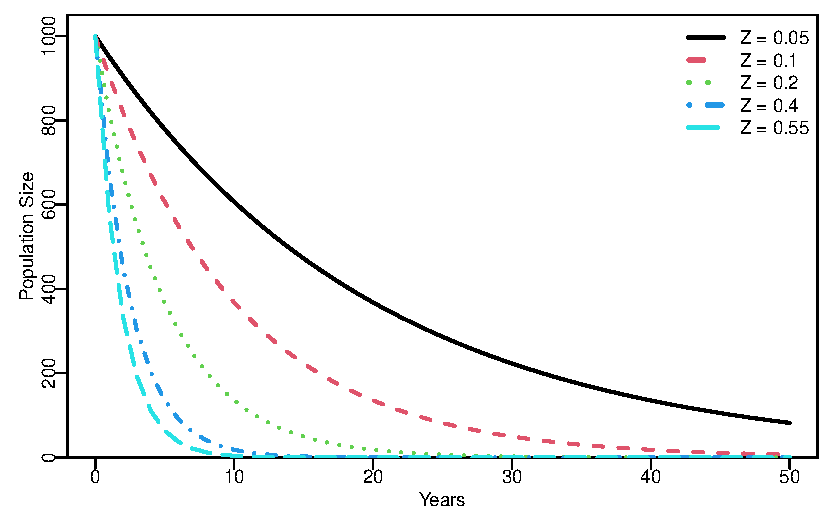
\includegraphics[keepaspectratio]{03-simpopmodel_files/figure-latex/fig3-6-1.pdf}}
\caption{\label{fig:fig3-6}Exponential population declines under different levels of total mortality. The top curve is Z = 0.05 and the steepest curve is Z = 0.55.}
\end{figure}

\subsection{瞬时 Vs 年死亡率}\label{ux77acux65f6-vs-ux5e74ux6b7bux4ea1ux7387}

在前一节中,我们讨论了所谓的瞬时率。它们可以用来生成残存率,即在给定瞬时死亡率的一年后预期残存的比例。瞬时死亡率的概念是指在无限小的时间段内的死亡率。

我们已经知道每年残存的比例:

\begin{equation}  
S={e}^{-Z}  
\label{eq:eq34}  
\end{equation}

因此1年时间死亡的比例表示为:

\begin{equation}  
A=1-{e}^{-Z}  
\label{eq:eq35}  
\end{equation}

如果只考虑瞬时捕捞死亡率\(F\),而忽略自然死亡率,则死亡的比例称为捕获率,\(H\)。

\begin{equation}  
H=1-{e}^{-F}  
\label{eq:eq36}  
\end{equation}

如果知道了每年的捕获率,就可以将其反向转换来估计瞬时捕捞死亡率。

\begin{equation}  
F=-\log{(1-H)}  
\label{eq:eq37}  
\end{equation}

其中对数是自然对数或以\(e\)为底的对数。

有时似乎很难直观地理解瞬时速率的含义。如果举例说明瞬时率是如何推导出来的,这个困难就会减轻。从1000个个体的种群开始,假设每年的移除率为\(0.5\),这意味着只有500个个体能存活一年。将年总死亡率代入最后一个方程,可估计瞬时总死亡率为\(-\log(1-0.5) = 0.693147\)。如果我们使用两个6个月周期来近似这个水平所需的时间步长,以获得50\%的存活率,我们需要将0.693147除以2.0,并将死亡率用2次。类似地,如果时间步长是每月的,我们将除以12,并将结果应用12次。虽然很难将每个月称为瞬时,但这将是适用近似瞬时死亡率(0.693147/12)的期间。这种重新缩放可以在越来越小的时间间隔中发生,直到时间间隔足够小,结果与预期的500个年终剩余个体没有显著差异,表(3.3)。

显而易见,应用近似瞬时速率的时间间隔越短,最终值就越接近预期的1000的0.5(即500)。希望这些代码能够帮助您对瞬时死亡率概念有直观的了解。

年死亡率可以与瞬时死亡率标绘出来,以说明两者之间的差异。请注意,大约在瞬时速率0.18的情况下,年收捕速率也大致相同。应该清楚的是,不可能获得大于1.0的捕获率(相当于捕获\textgreater100\%的可开发生物量)。高的捕获率开始显得难以置信,如果它们出现在适合渔业模式的情况下,那么在被接受之前,它们确实需要得到保护。另一方面,瞬时率显然可以超过1.0,但理想情况下,这样的事件不应再被误解。

\begin{Shaded}
\begin{Highlighting}[]
 \CommentTok{\#Prepare matrix of harvest rate vs time to appoximate F  }
\NormalTok{Z }\OtherTok{\textless{}{-}} \SpecialCharTok{{-}}\FunctionTok{log}\NormalTok{(}\FloatTok{0.5}\NormalTok{)  }
\NormalTok{timediv }\OtherTok{\textless{}{-}} \FunctionTok{c}\NormalTok{(}\DecValTok{2}\NormalTok{,}\DecValTok{4}\NormalTok{,}\DecValTok{12}\NormalTok{,}\DecValTok{52}\NormalTok{,}\DecValTok{365}\NormalTok{,}\DecValTok{730}\NormalTok{,}\DecValTok{2920}\NormalTok{,}\DecValTok{8760}\NormalTok{,}\DecValTok{525600}\NormalTok{)  }
\NormalTok{yrfrac }\OtherTok{\textless{}{-}} \DecValTok{1}\SpecialCharTok{/}\NormalTok{timediv  }
\FunctionTok{names}\NormalTok{(yrfrac) }\OtherTok{\textless{}{-}} \FunctionTok{c}\NormalTok{(}\StringTok{"6mth"}\NormalTok{,}\StringTok{"3mth"}\NormalTok{,}\StringTok{"1mth"}\NormalTok{,}\StringTok{"1wk"}\NormalTok{,}\StringTok{"1d"}\NormalTok{,}\StringTok{"12h"}\NormalTok{,  }
                   \StringTok{"3h"}\NormalTok{,}\StringTok{"1h"}\NormalTok{,}\StringTok{"1m"}\NormalTok{)  }
\NormalTok{nfrac }\OtherTok{\textless{}{-}} \FunctionTok{length}\NormalTok{(yrfrac)  }
\NormalTok{columns }\OtherTok{\textless{}{-}} \FunctionTok{c}\NormalTok{(}\StringTok{"yrfrac"}\NormalTok{,}\StringTok{"divisor"}\NormalTok{,}\StringTok{"yrfracH"}\NormalTok{,}\StringTok{"Remain"}\NormalTok{)  }
\NormalTok{result }\OtherTok{\textless{}{-}} \FunctionTok{matrix}\NormalTok{(}\DecValTok{0}\NormalTok{,}\AttributeTok{nrow=}\NormalTok{nfrac,}\AttributeTok{ncol=}\FunctionTok{length}\NormalTok{(columns),  }
                 \AttributeTok{dimnames=}\FunctionTok{list}\NormalTok{(}\FunctionTok{names}\NormalTok{(yrfrac),columns))  }
\ControlFlowTok{for}\NormalTok{ (i }\ControlFlowTok{in} \DecValTok{1}\SpecialCharTok{:}\NormalTok{nfrac) \{  }
\NormalTok{   timestepmort }\OtherTok{\textless{}{-}}\NormalTok{ Z}\SpecialCharTok{/}\NormalTok{timediv[i]   }
\NormalTok{   N }\OtherTok{\textless{}{-}} \DecValTok{1000}  
   \ControlFlowTok{for}\NormalTok{ (j }\ControlFlowTok{in} \DecValTok{1}\SpecialCharTok{:}\NormalTok{timediv[i]) N }\OtherTok{\textless{}{-}}\NormalTok{ N }\SpecialCharTok{*}\NormalTok{ (}\DecValTok{1}\SpecialCharTok{{-}}\NormalTok{timestepmort)  }
\NormalTok{   result[i,] }\OtherTok{\textless{}{-}} \FunctionTok{c}\NormalTok{(yrfrac[i],timediv[i],timestepmort,N)  }
\NormalTok{\}  }
\NormalTok{result}
\end{Highlighting}
\end{Shaded}

\begin{verbatim}
##            yrfrac divisor      yrfracH   Remain
## 6mth 5.000000e-01       2 3.465736e-01 426.9661
## 3mth 2.500000e-01       4 1.732868e-01 467.1104
## 1mth 8.333333e-02      12 5.776227e-02 489.6953
## 1wk  1.923077e-02      52 1.332975e-02 497.6748
## 1d   2.739726e-03     365 1.899033e-03 499.6706
## 12h  1.369863e-03     730 9.495167e-04 499.8354
## 3h   3.424658e-04    2920 2.373792e-04 499.9589
## 1h   1.141553e-04    8760 7.912639e-05 499.9863
## 1m   1.902588e-06  525600 1.318773e-06 499.9998
\end{verbatim}

\begin{Shaded}
\begin{Highlighting}[]
\CommentTok{\#Annual harvest rate against instantaneous F, Fig 3.7  }
\NormalTok{Fi }\OtherTok{\textless{}{-}} \FunctionTok{seq}\NormalTok{(}\FloatTok{0.001}\NormalTok{,}\DecValTok{2}\NormalTok{,}\FloatTok{0.001}\NormalTok{)  }
\NormalTok{H }\OtherTok{\textless{}{-}} \DecValTok{1} \SpecialCharTok{{-}} \FunctionTok{exp}\NormalTok{(}\SpecialCharTok{{-}}\NormalTok{Fi)  }
\FunctionTok{parset}\NormalTok{()  }\CommentTok{\# a wrapper for simplifying defining the par values  }
\FunctionTok{plot}\NormalTok{(Fi,H,}\AttributeTok{type=}\StringTok{"l"}\NormalTok{,}\AttributeTok{lwd=}\DecValTok{2}\NormalTok{,}\AttributeTok{panel.first=}\FunctionTok{grid}\NormalTok{(),  }
     \AttributeTok{xlab=}\StringTok{"Instantaneous Fishing Mortality F"}\NormalTok{,  }
     \AttributeTok{ylab=}\StringTok{"Annual Proportion Mortality H"}\NormalTok{)  }
\FunctionTok{lines}\NormalTok{(}\FunctionTok{c}\NormalTok{(}\DecValTok{0}\NormalTok{,}\DecValTok{1}\NormalTok{),}\FunctionTok{c}\NormalTok{(}\DecValTok{0}\NormalTok{,}\DecValTok{1}\NormalTok{),}\AttributeTok{lwd=}\DecValTok{2}\NormalTok{,}\AttributeTok{lty=}\DecValTok{2}\NormalTok{,}\AttributeTok{col=}\DecValTok{2}\NormalTok{)  }
\end{Highlighting}
\end{Shaded}

\begin{figure}
\centering
\pandocbounded{\includegraphics[keepaspectratio]{03-simpopmodel_files/figure-latex/fig3-7-1.pdf}}
\caption{\label{fig:fig3-7} The relationship between the instantaneous fishing mortality rate (solid line) and the annual fishing mortality or annual harvest rate (dashed line). The values diverge at values of F greater than about 0.2.}
\end{figure}

\section{简单单位补充量渔获量}\label{ux7b80ux5355ux5355ux4f4dux8865ux5145ux91cfux6e14ux83b7ux91cf}

我们知道,一旦某一世代补充到群体中,其数量只会减少(假设没有移入)。注意''补充量(recruitment)``的概念,它可以指后期仔鱼进入资源后,然而,它也可以指个体变得可用或易受渔业损害。这里我们关注的是仔鱼后加入资源后的情况。当我们在下面和\emph{静态模型(Static Models)}的章节中考虑选择性和可用性概念时,我们将处理补充量加入到渔业。有趣的是,尽管数字预计将减少通过时间,鉴于个体体长和重量上生长,我们还不知道如果世代的质量总是随时间减少或者增加然后减少最终所有的个体死亡。

一个世代的质量是否会在几年内增加,即使它的数量首次发现下降,因为对于捕获和努力之间的关系有一种简单但普遍的直觉。很明显,一种鱼类的渔获量总是会随着捕捞努力量的增加而增加,但这只是短期的想法。这个看似显而易见的概念在1930年之前就被驳斥了,并被Russell(1942)的一些出版著作很好地阐述了,他证明了一个渔业的最大持续渔获量不一定来自于最大努力量(或最大捕捞死亡)。这不仅是一个学术问题,而且直接关系到渔业的管理。一旦人们意识到过度捕捞甚至是鱼类资源崩溃的可能性,这一问题直到20世纪初才被正式承认(Garstang, 1900),那么如何最好地管理渔业就成为一个重要的问题。在管理渔业时,曾试图管理所作的全部努力量。支持这一观点的一个论点来自于单位补充量渔获量(yield-per-recruit,YPR)的概念,该概念以数量和质量的形式从数学上跟踪了在不同水平的强制捕捞死亡率下的世代的命运;捕捞死亡率被认为与所采取的努力量直接相关。``单位补充量''的概念意味着它遵循个体世代,并以最大化每个补充量的收益为目标。

我们将重复Russell(1942)的例子来说明YPR背后的思想。Russell的例子只涉及捕捞死亡率,这与假设没有自然死亡率(忽略了M)是一样的。对于这个简单的YPR我们也会忽略自然死亡率和应用一系列常数收获率每年计算年龄-数量(numbers-at-age)(相当于式\eqref{eq:eq33}),我们将使用一个年龄-体重乘以年龄-数量计算年龄-渔获量的重量,从中我们可以获得总的预期渔获量。

\begin{Shaded}
\begin{Highlighting}[]
\CommentTok{\# Simple Yield{-}per{-}Recruit see Russell (1942)  }
\NormalTok{age }\OtherTok{\textless{}{-}} \DecValTok{1}\SpecialCharTok{:}\DecValTok{11}\NormalTok{;  nage }\OtherTok{\textless{}{-}} \FunctionTok{length}\NormalTok{(age); N0 }\OtherTok{\textless{}{-}} \DecValTok{1000}  \CommentTok{\# some definitions  }
 \CommentTok{\# weight{-}at{-}age values  }
\NormalTok{WaA }\OtherTok{\textless{}{-}} \FunctionTok{c}\NormalTok{(}\ConstantTok{NA}\NormalTok{,}\FloatTok{0.082}\NormalTok{,}\FloatTok{0.175}\NormalTok{,}\FloatTok{0.283}\NormalTok{,}\FloatTok{0.4}\NormalTok{,}\FloatTok{0.523}\NormalTok{,}\FloatTok{0.7}\NormalTok{,}\FloatTok{0.85}\NormalTok{,}\FloatTok{0.925}\NormalTok{,}\FloatTok{0.99}\NormalTok{,}\FloatTok{1.0}\NormalTok{)  }
 \CommentTok{\# now the harvest rates  }
\NormalTok{H }\OtherTok{\textless{}{-}} \FunctionTok{c}\NormalTok{(}\FloatTok{0.01}\NormalTok{,}\FloatTok{0.06}\NormalTok{,}\FloatTok{0.11}\NormalTok{,}\FloatTok{0.16}\NormalTok{,}\FloatTok{0.21}\NormalTok{,}\FloatTok{0.26}\NormalTok{,}\FloatTok{0.31}\NormalTok{,}\FloatTok{0.36}\NormalTok{,}\FloatTok{0.55}\NormalTok{,}\FloatTok{0.8}\NormalTok{)  }
\NormalTok{nH }\OtherTok{\textless{}{-}} \FunctionTok{length}\NormalTok{(H)  }
\NormalTok{NaA }\OtherTok{\textless{}{-}} \FunctionTok{matrix}\NormalTok{(}\DecValTok{0}\NormalTok{,}\AttributeTok{nrow=}\NormalTok{nage,}\AttributeTok{ncol=}\NormalTok{nH,}\AttributeTok{dimnames=}\FunctionTok{list}\NormalTok{(age,H)) }\CommentTok{\# storage  }
\NormalTok{CatchN }\OtherTok{\textless{}{-}}\NormalTok{ NaA;  CatchW }\OtherTok{\textless{}{-}}\NormalTok{ NaA      }\CommentTok{\# define some storage matrices  }
\ControlFlowTok{for}\NormalTok{ (i }\ControlFlowTok{in} \DecValTok{1}\SpecialCharTok{:}\NormalTok{nH) \{                }\CommentTok{\# loop through the harvest rates  }
\NormalTok{   NaA[}\DecValTok{1}\NormalTok{,i] }\OtherTok{\textless{}{-}}\NormalTok{ N0  }\CommentTok{\# start each harvest rate with initial numbers  }
   \ControlFlowTok{for}\NormalTok{ (age }\ControlFlowTok{in} \DecValTok{2}\SpecialCharTok{:}\NormalTok{nage) \{  }\CommentTok{\# loop through over{-}simplified dynamics  }
\NormalTok{      NaA[age,i] }\OtherTok{\textless{}{-}}\NormalTok{ NaA[(age}\DecValTok{{-}1}\NormalTok{),i] }\SpecialCharTok{*}\NormalTok{ (}\DecValTok{1} \SpecialCharTok{{-}}\NormalTok{ H[i])  }
\NormalTok{      CatchN[age,i] }\OtherTok{\textless{}{-}}\NormalTok{ NaA[(age}\DecValTok{{-}1}\NormalTok{),i] }\SpecialCharTok{{-}}\NormalTok{ NaA[age,i]  }
\NormalTok{   \}  }
\NormalTok{   CatchW[,i] }\OtherTok{\textless{}{-}}\NormalTok{ CatchN[,i] }\SpecialCharTok{*}\NormalTok{ WaA  }
\NormalTok{\}                      }\CommentTok{\# transpose the vector of total catches to  }
\NormalTok{totC }\OtherTok{\textless{}{-}} \FunctionTok{t}\NormalTok{(}\FunctionTok{colSums}\NormalTok{(CatchW,}\AttributeTok{na.rm=}\ConstantTok{TRUE}\NormalTok{))   }\CommentTok{\# simplify later printing  }
\end{Highlighting}
\end{Shaded}

不同的捕获率对种群年龄结构的影响在渔获的分年龄数量和分年龄重量上都很明显。随着捕获率的增加,年龄较大的组中的年龄捕获数越来越少,分年龄捕获数也越来越少。对于较高的捕获率,种群变得依赖于最近的补充量,而不是在较老的年龄组中数量和生物量的积累。

如果使用\textbf{MQMF}中的\texttt{plot1()}函数绘制渔获总重量对捕获率的图,我们可以立即看到,在产量方面确实存在一个最佳渔获率,而不是最大利用率。如果让努力量增加,渔获量并不总是增加。如果捕获率很低,那么捕获的鱼类太少,不足以弥补显著的捕获量。然而,产量随着捕获率的增加而迅速增加,而当超过产生最大产量的捕获率时,产量下降得更慢。

\begin{Shaded}
\begin{Highlighting}[]
 \CommentTok{\#Use MQMF::plot1 for a quick plot of the total catches. Figure 3.8  }
\FunctionTok{plot1}\NormalTok{(H,totC,}\AttributeTok{xlab=}\StringTok{"Harvest Rate"}\NormalTok{,}\AttributeTok{ylab=}\StringTok{"Total Yield"}\NormalTok{,}\AttributeTok{lwd=}\DecValTok{2}\NormalTok{)  }
\end{Highlighting}
\end{Shaded}

\begin{figure}
\centering
\pandocbounded{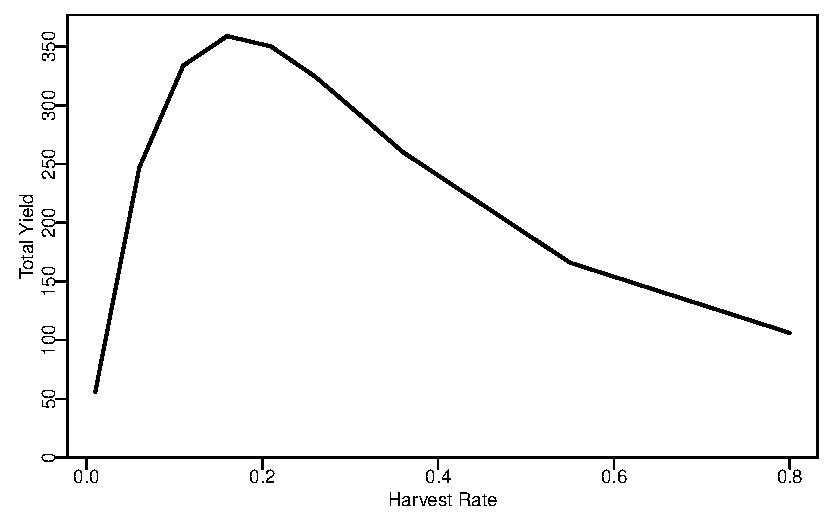
\includegraphics[keepaspectratio]{03-simpopmodel_files/figure-latex/fig3-8-1.pdf}}
\caption{\label{fig:fig3-8}A simplified yield-per-recruit analysis that ignores natural mortality, selectivity-at-age, or any other influences. This analysis uses some weight-at-age data from Russell, 1942 although a wider array of harvest rates were examined than just the two by Russell.}
\end{figure}

为了快速说明不同捕获率的影响,这个例子在1942年获得了成功。对单位补充量渔获量的更全面的处理需要考虑动态中的自然死亡率和网具选择性带来的年龄死亡率差异。

\subsection{单位补充量渔获量中的选择性}\label{ux5355ux4f4dux8865ux5145ux91cfux6e14ux83b7ux91cfux4e2dux7684ux9009ux62e9ux6027}

通常,在完全年龄结构的渔业模型中,人们会实现一个选择性函数来描述每个年龄组(或体长组)对特定捕捞网具的不同脆弱性。随着鱼变老(或变大),它们会越来越多地补充到渔业中,直到它们完全容易受到捕捞的影响。通常,这种选择性曲线的参数是在将年龄结构模型与渔业数据拟合的过程中获得的。然而,在这里,我们将仅仅是给定了属性值(参见\emph{静态模型(static Models)}一章中选择性的更多细节)。早期的YPR分析经常使用所谓的刀刃选择性,这意味着鱼类在特定年龄100\%容易受到渔具的攻击。然而,在这里,我们将实现一个更现实、但更简单的脆弱性随年龄的选择性曲线。有许多不同的方程用来描述不同渔具的选择性特性,但拖网渔具使用的一个非常常见的方程是标准logistic或s形曲线,它也可以有许多公式化的表达式。一个常用来描述随年龄\(S_a\) 或体长变化,选择性logistic形状 ,以及年龄或体长的成熟度定义为:

\begin{equation}  
{{s}_{a}}=\frac{1}{1+{{({{e}^{(\alpha +\beta a)}})}^{-1}}}=\frac{{{e}^{(\alpha +\beta a)}}}{1+{{e}^{(\alpha +\beta a)}}}  
\label{eq:eq38} 
\end{equation}

式中\(\alpha\) 和 \(\beta\)为logistic参数,\(-\alpha/\beta\) 为0.5(50\%)选择性处的年龄。四分位数之间的距离(字面上分位数的25\%到75\%;logistic曲线梯度的度量)定义为\(IQ=2\log(3)/\beta\)(参见\textbf{MQMF}函数\texttt{mature()}用于该函数的执行)。一般来说,在年龄结构模型中,需要长度或年龄组成数据,以便直接估计网具选择性和渔业可用性。在计算单位补充量渔获量时,通常的理由是要包括一种形式的选择性,以确定开始应用捕捞死亡率的最佳年龄。在管理方面,这可以用来确定拖网或刺网的网眼尺寸。这就是为什么刀刃选择性经常被使用的原因,它可以识别年龄在什么年龄以下没有选择,在什么年龄以上有100\%的选择。这在\textbf{MQMF}函数\texttt{logistic()}中实现(使用不同的公式),但在\texttt{mature()}中没有实现。刀刃选择性并不倾向于在完整的年龄结构种群评估模型中使用。

\begin{Shaded}
\begin{Highlighting}[]
 \CommentTok{\#Logistic S shaped cureve for maturity  }
\NormalTok{ages }\OtherTok{\textless{}{-}} \FunctionTok{seq}\NormalTok{(}\DecValTok{0}\NormalTok{,}\DecValTok{50}\NormalTok{,}\DecValTok{1}\NormalTok{)  }
\NormalTok{sel1 }\OtherTok{\textless{}{-}} \FunctionTok{mature}\NormalTok{(}\SpecialCharTok{{-}}\FloatTok{3.650425}\NormalTok{,}\FloatTok{0.146017}\NormalTok{,}\AttributeTok{sizeage=}\NormalTok{ages) }\CommentTok{\#{-}3.65/0.146=25  }
\NormalTok{sel2 }\OtherTok{\textless{}{-}} \FunctionTok{mature}\NormalTok{(}\SpecialCharTok{{-}}\DecValTok{6}\NormalTok{,}\FloatTok{0.2}\NormalTok{,ages)  }
\NormalTok{sel3 }\OtherTok{\textless{}{-}} \FunctionTok{mature}\NormalTok{(}\SpecialCharTok{{-}}\DecValTok{6}\NormalTok{,}\FloatTok{0.24}\NormalTok{,ages)  }
\FunctionTok{plot1}\NormalTok{(ages,sel1,}\AttributeTok{xlab=}\StringTok{"Age Yrs"}\NormalTok{,}\AttributeTok{ylab=}\StringTok{"Selectivity"}\NormalTok{,}\AttributeTok{cex=}\FloatTok{0.75}\NormalTok{,}\AttributeTok{lwd=}\DecValTok{2}\NormalTok{)  }
\FunctionTok{lines}\NormalTok{(ages,sel2,}\AttributeTok{col=}\DecValTok{2}\NormalTok{,}\AttributeTok{lwd=}\DecValTok{2}\NormalTok{,}\AttributeTok{lty=}\DecValTok{2}\NormalTok{)  }
\FunctionTok{lines}\NormalTok{(ages,sel3,}\AttributeTok{col=}\DecValTok{3}\NormalTok{,}\AttributeTok{lwd=}\DecValTok{2}\NormalTok{,}\AttributeTok{lty=}\DecValTok{3}\NormalTok{)  }
\FunctionTok{abline}\NormalTok{(}\AttributeTok{v=}\DecValTok{25}\NormalTok{,}\AttributeTok{col=}\StringTok{"grey"}\NormalTok{,}\AttributeTok{lty=}\DecValTok{2}\NormalTok{)   }
\FunctionTok{abline}\NormalTok{(}\AttributeTok{h=}\FunctionTok{c}\NormalTok{(}\FloatTok{0.25}\NormalTok{,}\FloatTok{0.5}\NormalTok{,}\FloatTok{0.75}\NormalTok{),}\AttributeTok{col=}\StringTok{"grey"}\NormalTok{,}\AttributeTok{lty=}\DecValTok{2}\NormalTok{)  }
\FunctionTok{legend}\NormalTok{(}\StringTok{"topleft"}\NormalTok{,}\FunctionTok{c}\NormalTok{(}\StringTok{"25\_15.04"}\NormalTok{,}\StringTok{"30\_10.986"}\NormalTok{,}\StringTok{"25\_9.155"}\NormalTok{),}\AttributeTok{col=}\FunctionTok{c}\NormalTok{(}\DecValTok{1}\NormalTok{,}\DecValTok{2}\NormalTok{,}\DecValTok{3}\NormalTok{),  }
       \AttributeTok{lwd=}\DecValTok{3}\NormalTok{,}\AttributeTok{cex=}\FloatTok{1.1}\NormalTok{,}\AttributeTok{bty=}\StringTok{"n"}\NormalTok{,}\AttributeTok{lty=}\DecValTok{1}\SpecialCharTok{:}\DecValTok{3}\NormalTok{)  }
\end{Highlighting}
\end{Shaded}

\begin{figure}
\centering
\pandocbounded{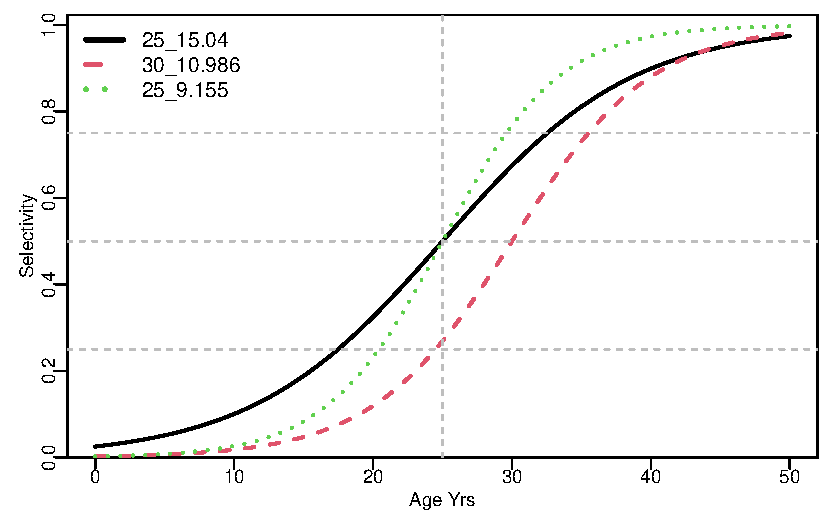
\includegraphics[keepaspectratio]{03-simpopmodel_files/figure-latex/fig3-9-1.pdf}}
\caption{\label{fig:fig3-9}Examples of the logistic S-shaped curve using the mature() function. The legend consists of the L50 and the IQ for each curve with their parameters defined in the code.}
\end{figure}

\subsection{Baranov 渔获量方程}\label{baranov-ux6e14ux83b7ux91cfux65b9ux7a0b}

式\eqref{eq:eq34}描述了结合捕捞和自然死亡后的残存率,但简单的总死亡率 \(Z\)意味着所有鱼的捕捞死亡率相同。如果我们要考虑选择性,那么我们需要考虑年龄的捕捞死亡率。

\begin{equation}  
S_{a,t}=e^{-(M + {s_a}{F_t})}  
\label{eq:eq39} 
\end{equation}

其中\(S_{a,t}\) 为\(t\)年\(a\)龄鱼的残存率,\(M\)为自然死亡系数(假设随时间不变),\(s_a\)为年龄\(a\)的选择性,\(F_t\)已知,\(t\)年完全选择的捕捞死亡系数。

一旦残存数量\(S_tN_t\)已知,那么死亡的数量显然不同时期存在差异。从一个时间段到下一个时间段一个世代的死亡总数量可以表示为:

\begin{equation}  
N_{z}=N_{t}-N_{t+1}  
\label{eq:eq310}  
\end{equation}

如果用残存等式代替\(N_{t_1}\),就可得到残存的补偿方程,其描述了时间段间总死亡数量:

\begin{equation}  
N_{a,z}=N_{a,t}-N_{a,t}{e}^{-(M+{s_a}{F_t})}=N_{a,t}(1-{e}^{-(M+{s_a}{F_t})})  
\label{eq:eq311}  
\end{equation}

这里\(N_{a,z}\)为年龄\(a\)死亡的数量。当然,不是所有死亡的鱼都作为渔获,一些是自然死亡的,但也出现捕捞一些自然死亡的个体的现象。将死亡率分为\(M\)(假设不同年龄的自然死亡系数不变)和\(F_t\)(捕捞努力量引起的完全选择死亡),它可以随时间\(t\)而变化,可以计算渔获量和残存量。可以将\(s_aF_t\)简化为\(F_{a,t}\)。有可能进行这种分开的假设是年龄结构和体长结构的种群评估模型的一个重要组成部分。使用瞬时率,由于捕捞死亡而非自然死亡的数量用分数\(F_{a,t}/(M+F_{a,t})\)来描述,如果将其包含到\eqref{eq:eq311}中,我们发现我们已经推导出了所谓的Baranov 渔获量方程(Quinn, 2003;Quinn 和Deriso,1999),现在通常用于渔业建模,以估计渔获中的数量。它被用来追踪单个世代的命运,如果将所有年龄段相加,就能得出总的渔获量:

\begin{equation}  
{{\hat{C}}_{a,t}}=\frac{{F}_{a,t}}{M+{F}_{a,t}}{{N}_{a,t}}\left( 1-{{e}^{-\left( M+{{F}_{a,t}} \right)}} \right)  
(\#eq:eq312)  
\end{equation}

其中\(\hat{C}_{a,t}\)为\(t\)年年龄\(a\)的期望渔获,\(F_{a,t}\)为\(t\)年年龄\(a\)的瞬时捕捞死亡系率(\(s_aF_t\)),\(M\)为自然死亡率(假设年龄间不变),\(N_{a,t}\)为\(t\)年年龄\(a\)的数量。该方程可用\textbf{MQMF}的函数\texttt{bce()}运行。

\begin{Shaded}
\begin{Highlighting}[]
 \CommentTok{\# Baranov catch equation  }
\NormalTok{age }\OtherTok{\textless{}{-}} \DecValTok{0}\SpecialCharTok{:}\DecValTok{12}\NormalTok{;  nage }\OtherTok{\textless{}{-}} \FunctionTok{length}\NormalTok{(age)   }
\NormalTok{sa }\OtherTok{\textless{}{-}}\FunctionTok{mature}\NormalTok{(}\SpecialCharTok{{-}}\DecValTok{4}\NormalTok{,}\DecValTok{2}\NormalTok{,age) }\CommentTok{\#selectivity{-}at{-}age  }
\NormalTok{H }\OtherTok{\textless{}{-}} \FloatTok{0.2}\NormalTok{;  M }\OtherTok{\textless{}{-}} \FloatTok{0.35}  
\NormalTok{FF }\OtherTok{\textless{}{-}} \SpecialCharTok{{-}}\FunctionTok{log}\NormalTok{(}\DecValTok{1} \SpecialCharTok{{-}}\NormalTok{ H)}\CommentTok{\#Fully selected instantaneous fishing mortality  }
\NormalTok{Ft }\OtherTok{\textless{}{-}}\NormalTok{ sa }\SpecialCharTok{*}\NormalTok{ FF     }\CommentTok{\# instantaneous Fishing mortality{-}at{-}age  }
\NormalTok{N0 }\OtherTok{\textless{}{-}} \DecValTok{1000}  
\NormalTok{out }\OtherTok{\textless{}{-}} \FunctionTok{cbind}\NormalTok{(}\FunctionTok{bce}\NormalTok{(M,Ft,N0,age),}\StringTok{"Select"}\OtherTok{=}\NormalTok{sa)  }\CommentTok{\# out becomes Table 3.7  }
\NormalTok{out}
\end{Highlighting}
\end{Shaded}

\begin{verbatim}
##             Nt     N-Dying      Catch     Select
## 0  1000.000000          NA         NA 0.01798621
## 1   686.190932 291.6446082 22.1644597 0.11920292
## 2   432.500784 192.3678101 61.3223376 0.50000000
## 3   250.395070 116.6182009 65.4875131 0.88079708
## 4   141.728025  66.8273729 41.8396720 0.98201379
## 5    79.943338  37.7662423 24.0184454 0.99752738
## 6    45.071467  21.2978904 13.5739804 0.99966465
## 7    25.409318  12.0072427  7.6549061 0.99995460
## 8    14.324535   6.7691305  4.3156530 0.99999386
## 9     8.075465   3.8161037  2.4329663 0.99999917
## 10    4.552547   2.1513305  1.3715871 0.99999989
## 11    2.566501   1.2128136  0.7732329 0.99999998
## 12    1.446866   0.6837242  0.4359104 1.00000000
\end{verbatim}

\subsection{生长和各年龄体重}\label{ux751fux957fux548cux5404ux5e74ux9f84ux4f53ux91cd}

为了获得渔获量的质量(即渔获量的重量),需要将渔获量中的各年龄数量乘以各年龄重量。各年龄体重可以是特定年份特定渔业的平均体重观测值的向量(Beverton and Holt, 1957),或者,更常见的是,从von Bertalanffy生长曲线推导出的标准年龄体重方程,它从各年龄长度开始。

\begin{equation}  
L_{a}=L_{\infty}(1-e^{(-K(a-t_0))})  
\label{eq:eq313}  
\end{equation}

其中,\(L_a\)为年龄\(a\)的长度,\(L_{\infty}\)为平均最大年龄长度,\(K\)为系数,它决定了如何快速达到\(L_{\infty}\),\(t_0\)为长度为0时的假设年龄。用\textbf{MQMF}的函数\texttt{vB()}运行。假设各年龄长度和各年龄体重之间存在幂次关系,因此增加了两个参数:

\begin{equation}  
\begin{split}  
{W_a}  &= {\alpha}{L_a}^{b}=w_a(1-e^{(-K(a-t_0))})^{b} \\  
{\log{(W_a)}} &= \log{(\alpha)}+{b}{L_a}  
\end{split}  
\label{eq:eq314}  
\end{equation}

其中,\(\alpha\)为恒定值,\(w_a\)为\((\alpha L_{\infty})\),\(b\)为指数,近似为3.0(大小是二维的,而重量是三维的)。对数变换形式当然是线性的。在\emph{静态模型(Static Models)}一章中,我们将看到如何估计这些模型的参数。

\section{完整的单位补充量产量}\label{ux5b8cux6574ux7684ux5355ux4f4dux8865ux5145ux91cfux4ea7ux91cf}

把所有这些整合在一起,意味着我们可以产生一个更完整的单位补充量产量(YPR)分析。标准的YPR分析假设恒定的补充量,这意味着我们可以跟踪单个世代的命运,并仍然捕捉所需的细节。当然,补充量不是一个常数,所以这种方法被认为是基于长期或平衡条件。以这种方式忽略变化和随机性意味着,任何关于潜在生产力和由此产生的管理决策的结论都需要谨慎对待(事实上,非常谨慎)。但这些方法是在渔业分析都是确定性的,并假定处于平衡状态时发展起来的,不确定性的含义尚未被探索(Beverton和Holt, 1957)。

当目标是最大化产量时,这样的分析是有意义的。但是,恒定补充量的假设和对不确定性的忽视意味着这些分析通常不是保守的。人们尝试改进YPR分析提出的建议,其中比较有用的是\(F_{0.1}\)的出现(发音为F zero point one)。定义为产量曲线起点处产量增加率是1/10的渔获率(Hilborn和Walters, 1992)。\(F_{0.1}\)的优势这是捕捞努力量的相对 大幅下降,只会导致产量的很小损失。这可以提高渔业的经济效益和可持续性。然而,本质上使用\(F_{0.1}\) 仍然是一个经验规则,它在实践中比\(F_{max}\)(最高产量点)更可持续,通常比\(F_{msy}\)(平衡时可产生MSY的捕捞死亡率)更好。

\begin{Shaded}
\begin{Highlighting}[]
\CommentTok{\# A more complete YPR analysis  }
\NormalTok{age }\OtherTok{\textless{}{-}} \DecValTok{0}\SpecialCharTok{:}\DecValTok{20}\NormalTok{;  nage }\OtherTok{\textless{}{-}} \FunctionTok{length}\NormalTok{(age) }\CommentTok{\#storage vectors and matrices  }
\NormalTok{laa }\OtherTok{\textless{}{-}} \FunctionTok{vB}\NormalTok{(}\FunctionTok{c}\NormalTok{(}\FloatTok{50.0}\NormalTok{,}\FloatTok{0.25}\NormalTok{,}\SpecialCharTok{{-}}\FloatTok{1.5}\NormalTok{),age) }\CommentTok{\# length{-}at{-}age  }
\NormalTok{WaA }\OtherTok{\textless{}{-}}\NormalTok{ (}\FloatTok{0.015} \SpecialCharTok{*}\NormalTok{ laa }\SpecialCharTok{\^{}} \FloatTok{3.0}\NormalTok{)}\SpecialCharTok{/}\DecValTok{1000}  \CommentTok{\# weight{-}at{-}age as kg  }
\NormalTok{H }\OtherTok{\textless{}{-}} \FunctionTok{seq}\NormalTok{(}\FloatTok{0.01}\NormalTok{,}\FloatTok{0.65}\NormalTok{,}\FloatTok{0.05}\NormalTok{);  nH }\OtherTok{\textless{}{-}} \FunctionTok{length}\NormalTok{(H)     }
\NormalTok{FF }\OtherTok{\textless{}{-}} \FunctionTok{round}\NormalTok{(}\SpecialCharTok{{-}}\FunctionTok{log}\NormalTok{(}\DecValTok{1} \SpecialCharTok{{-}}\NormalTok{ H),}\DecValTok{5}\NormalTok{)  }\CommentTok{\# Fully selected fishing mortality  }
\NormalTok{N0 }\OtherTok{\textless{}{-}} \DecValTok{1000}  
\NormalTok{M }\OtherTok{\textless{}{-}} \FloatTok{0.1}  
\NormalTok{numt }\OtherTok{\textless{}{-}} \FunctionTok{matrix}\NormalTok{(}\DecValTok{0}\NormalTok{,}\AttributeTok{nrow=}\NormalTok{nage,}\AttributeTok{ncol=}\NormalTok{nH,}\AttributeTok{dimnames=}\FunctionTok{list}\NormalTok{(age,FF))  }
\NormalTok{catchN }\OtherTok{\textless{}{-}} \FunctionTok{matrix}\NormalTok{(}\DecValTok{0}\NormalTok{,}\AttributeTok{nrow=}\NormalTok{nage,}\AttributeTok{ncol=}\NormalTok{nH,}\AttributeTok{dimnames=}\FunctionTok{list}\NormalTok{(age,FF))  }
\NormalTok{as50 }\OtherTok{\textless{}{-}} \FunctionTok{c}\NormalTok{(}\DecValTok{1}\NormalTok{,}\DecValTok{2}\NormalTok{,}\DecValTok{3}\NormalTok{)    }
\NormalTok{yield }\OtherTok{\textless{}{-}} \FunctionTok{matrix}\NormalTok{(}\DecValTok{0}\NormalTok{,}\AttributeTok{nrow=}\NormalTok{nH,}\AttributeTok{ncol=}\FunctionTok{length}\NormalTok{(as50),}\AttributeTok{dimnames=}\FunctionTok{list}\NormalTok{(H,as50))  }
\ControlFlowTok{for}\NormalTok{ (sel }\ControlFlowTok{in} \DecValTok{1}\SpecialCharTok{:}\FunctionTok{length}\NormalTok{(as50)) \{  }
\NormalTok{   sa }\OtherTok{\textless{}{-}} \FunctionTok{logist}\NormalTok{(as50[sel],}\FloatTok{1.0}\NormalTok{,age)  }\CommentTok{\# selectivity{-}at{-}age  }
   \ControlFlowTok{for}\NormalTok{ (harv }\ControlFlowTok{in} \DecValTok{1}\SpecialCharTok{:}\NormalTok{nH) \{  }
\NormalTok{      Ft }\OtherTok{\textless{}{-}}\NormalTok{ sa }\SpecialCharTok{*}\NormalTok{ FF[harv]      }\CommentTok{\# Fishing mortality{-}at{-}age  }
\NormalTok{      out }\OtherTok{\textless{}{-}} \FunctionTok{bce}\NormalTok{(M,Ft,N0,age)  }
\NormalTok{      numt[,harv] }\OtherTok{\textless{}{-}}\NormalTok{ out[,}\StringTok{"Nt"}\NormalTok{]  }
\NormalTok{      catchN[,harv] }\OtherTok{\textless{}{-}}\NormalTok{ out[,}\StringTok{"Catch"}\NormalTok{]  }
\NormalTok{      yield[harv,sel] }\OtherTok{\textless{}{-}} \FunctionTok{sum}\NormalTok{(out[,}\StringTok{"Catch"}\NormalTok{] }\SpecialCharTok{*}\NormalTok{ WaA,}\AttributeTok{na.rm=}\ConstantTok{TRUE}\NormalTok{)  }
\NormalTok{   \} }\CommentTok{\# end of harv loop  }
\NormalTok{\} }\CommentTok{\# end of sel loop  }
\end{Highlighting}
\end{Shaded}

\begin{Shaded}
\begin{Highlighting}[]
\CommentTok{\#A full YPR analysis  Figure 3.10  }
\FunctionTok{plot1}\NormalTok{(H,yield[,}\DecValTok{3}\NormalTok{],}\AttributeTok{xlab=}\StringTok{"Harvest Rate"}\NormalTok{,}\AttributeTok{ylab=}\StringTok{"Yield"}\NormalTok{,}\AttributeTok{cex=}\FloatTok{0.75}\NormalTok{,}\AttributeTok{lwd=}\DecValTok{2}\NormalTok{)  }
\FunctionTok{lines}\NormalTok{(H,yield[,}\DecValTok{2}\NormalTok{],}\AttributeTok{lwd=}\DecValTok{2}\NormalTok{,}\AttributeTok{col=}\DecValTok{2}\NormalTok{,}\AttributeTok{lty=}\DecValTok{2}\NormalTok{)  }
\FunctionTok{lines}\NormalTok{(H,yield[,}\DecValTok{1}\NormalTok{],}\AttributeTok{lwd=}\DecValTok{2}\NormalTok{,}\AttributeTok{col=}\DecValTok{3}\NormalTok{,}\AttributeTok{lty=}\DecValTok{3}\NormalTok{)  }
\FunctionTok{legend}\NormalTok{(}\StringTok{"bottomright"}\NormalTok{,}\AttributeTok{legend=}\NormalTok{as50,}\AttributeTok{col=}\FunctionTok{c}\NormalTok{(}\DecValTok{3}\NormalTok{,}\DecValTok{2}\NormalTok{,}\DecValTok{1}\NormalTok{),}\AttributeTok{lwd=}\DecValTok{3}\NormalTok{,}\AttributeTok{bty=}\StringTok{"n"}\NormalTok{,  }
       \AttributeTok{cex=}\FloatTok{1.0}\NormalTok{,}\AttributeTok{lty=}\FunctionTok{c}\NormalTok{(}\DecValTok{3}\NormalTok{,}\DecValTok{2}\NormalTok{,}\DecValTok{1}\NormalTok{))   }
\end{Highlighting}
\end{Shaded}

\begin{figure}
\centering
\pandocbounded{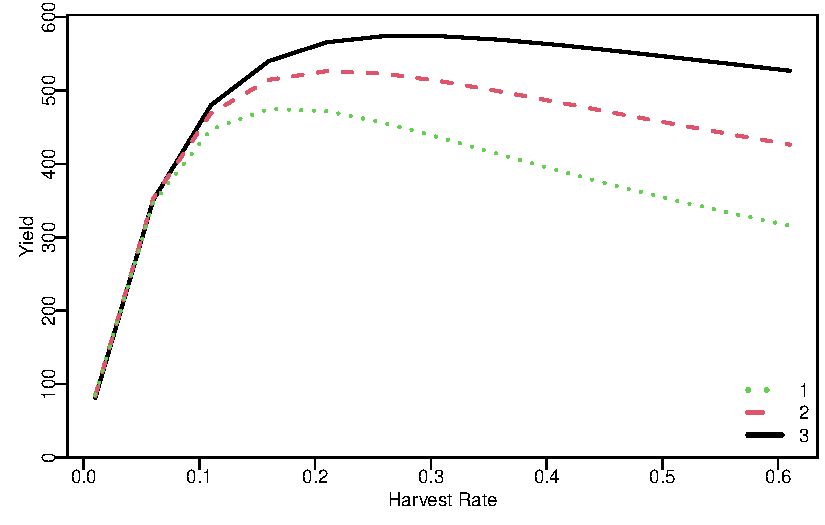
\includegraphics[keepaspectratio]{03-simpopmodel_files/figure-latex/fig3-10-1.pdf}}
\caption{\label{fig:fig3-10}The effect on the total equilibrium yield of applying different harvest rates and different ages of first exploitation. The legend identifies the different age of first exploitation.}
\end{figure}

这些详细的分析考虑了选择性、年龄体重和自然死亡率,提供了一个渔场在不同条件下的潜在产量的更准确的表示,尽管仍然是确定性的。一旦考虑到不确定性和自然变化,即使只是近似地使用\(F_{0.1}\) ,那么YPR分析仍然可以为了解特定渔业的生产能力提供一些有用的见解。当然,如今onbe更有可能进行单位补充量的利润分析,但原则是不变的。

\section{结束语}\label{ux7ed3ux675fux8bed-1}

我们使用了相对简单的种群模型来说明渔业和生态学中的许多观点。重要的是,重点是模拟模型,而不是将模型与数据拟合(见下一章模型参数估计)。模拟模型通常包括模型参数值的不确定性,但是,由于许多题目在这里只作了介绍性的处理,更彻底的处理本身需要一本书。然而,通过探索在考虑的各种模型上施加一系列参数值的含义,这些模型的属性和隐含的动力学可以被揭示出来。因此,模拟研究是对任何自然过程建模的重要工具。然而,同样重要的是,使用这些参数的合理或现实的组合进行模拟。理解所有模型的数学性质是很有用的,但是,自然地,最重要的兴趣是当模型具有现实值并可能在自然界中找到时。

在使用任何种群模型或其组成部分时获得的直觉对理解任何未来的工作都有价值,但是,当然,所说明的每个模型(特别是相对简单的模型)中的上下文和假设总是要记住的。令人惊讶的是,即使是简单的模型有时也能提供对各种自然过程的洞察。

在本章中,我们只考虑了简单的种群模型,但我们也可以很好地使用R来探索物种之间在竞争、捕食、寄生、共生等过程中的相互作用。所有的早期模型(Lotka,1925;Wolterra,1927;Gause,1934)考虑了没有空间结构的种群。使用R会相对直接地增加这种模型的复杂性,并包括空间细节,如Huffaker(1958)的实验探索。Huffaker后来的一些实验性捕食者-补捕食者安排持续了490天。在这种情况下,模拟研究对于扩展探索的可能性非常有用。这样有趣的工作将需要成为另一本书的一部分,因为在渔业领域,我们还有许多其他领域需要探索和讨论。

使用R作为进行此类模拟的工具,使得分析比在电子表格上布置参数操作更抽象。然而,代码块和已开发函数的可重用性,以及更复杂模型和函数的增量开发的潜力所带来的优势,超过了编程环境的更抽象的本质。使用R作为一种编程语言来开发这些不同的分析非常适合渔业和生态建模工作。

\begin{center}\rule{0.5\linewidth}{0.5pt}\end{center}

\chapter{模型参数估算}\label{ux6a21ux578bux53c2ux6570ux4f30ux7b97}

\section{简介}\label{ux7b80ux4ecb-3}

生态学和渔业学学建模的一个更重要的方面涉及到模型与数据的拟合。这种模型拟合需要:

\begin{itemize}
\item
  从对自然感兴趣的过程中获得的数据(样本、观测),
\item
  明确地选择一个适合手头任务的模型结构(模型设计,然后选择------大的主题本身),
\item
  明确地选择概率密度函数来表示当比较时,模拟过程的预测将如何不同于自然观测的预期分布(选择残差结构) ,最后,
\item
  寻找模型参数,优化之间的预测模型和任何观测数据(模型拟合的准则)匹配。
\end{itemize}

在上面的最后一个需求中,将模型与数据相匹配时所涉及的许多技巧/诡计/魔术都集中在那个看起来无害的单词或概念上进行\textbf{优化}。这是一个几乎是恶作剧的想法,有时会导致一个人陷入麻烦,虽然它也是一个挑战,往往是有趣的。生成所谓\emph{最佳拟合}模型的不同方法是本章的重点。它围绕着在描述模型的质量拟合可用数据时使用什么标准的想法,以及如何实现明确选择的标准。

我一直使用''明确的''这个词,并且有很好的理由,但是需要一些澄清。很多人都有过对数据进行线性回归拟合的经验,但是,根据我的经验,很少有人意识到,当他们拟合这样一个模型时,他们假设使用了加性正态随机残差(正态误差) ,并且他们正在最小化这些残差的平方和。根据上述四个要求,当将一个线性回归应用到一个数据集时,线性关系的假设回答了第二个要求,正态误差的使用(附加常数方差的假设)回答了第三个要求,平方和的最小化是满足第四个要求的选择。通常情况下,最好是明确地了解自己在做什么,而不是仅仅出于习惯或模仿他人。为了对这些模型拟合需求做出最合适的选择(即做出可以辩护的选择) ,分析师还需要了解被建模的自然过程。一个人可以假设和断言几乎任何事情,但只有这样的选择可以得到有效的辩护。作为一个更一般的陈述,如果一个人不能为一组选择辩护,那么他就不应该做出这些选择。

\subsection{最优化}\label{ux6700ux4f18ux5316}

在Microsoft Excel中,当对数据进行模型拟合时,使用内置的Excel解算器找到最佳模型参数。这包括设置电子表格,使最佳拟合标准(平方和、最大似然等,见下文)由一个单元格的内容表示,而模型参数和使用的数据则包含在其他相互关联的单元格中。改变一个模型的参数会改变产生的预测值,这反过来又会改变最佳拟合的标准值。一个 ``最佳''参数集可以通过寻找能优化观察值和预测值之间的匹配的参数来找到。这听起来很简单,但实际上是一门艺术,其中要做许多假设和决定。在Excel求解器中,人们确定了包含模型参数的单元格,然后求解器的内部代码将修改这些值,同时监测 ``最佳拟合标准''单元格,直到找到一个最小(或最大)值(或遇到一个例外)。实际上,这样的电子表格设置构成了在Excel中使用求解器的语法。我们将在R中使用求解器或优化函数,它们也有一个必要的语法,但它并不比设置电子表格更复杂,只是更抽象而已。

当对单一数据集(如年龄-长度)用2至6个参数进行非动态过程建模时,模型拟合通常是相对简单的。然而,当处理一个种群的动态过程时,可能会变得更加复杂,涉及到补充、个体生长、自然死亡和多个捕鱼船队的捕捞死亡。可能有许多类型的数据,可能有多于几十个甚至几百个参数。在这种情况下,为了调整预测值与观测值的拟合质量,必须使用某种形式的自动优化或非线性求解器。

优化是一个非常大的研究课题,在CRAN任务视图中详细讨论了许多可用的选项。在CRAN任务视图:优化和数学编程中可以找到详细的讨论,网址是\url{https://cran.r-project.org/}。在这里的工作中,我们将主要使用内置的函数\texttt{nlm()}(尝试 \texttt{?nlm}),但也有许多替代方法(包括\texttt{nlminb()}、\texttt{optim()}等)。如果你要参与模型拟合,那么真的值得阅读R-CRAN上关于优化的任务视图,并且作为第一步,探索 \texttt{nlm()} 和 \texttt{optim()} 函数的帮助和例子。

有时有可能猜测出一组参数,产生看似合理的可视拟合,至少对简单的静态模型来说是如此。然而,虽然这种通过\emph{目测拟合}(fitting-by-eye)可以为估计模型的参数提供可用的起点,但它并不构成将模型与数据拟合的可辩护的标准。这是因为我的 ``目测拟合''(或称 ``黑暗中的狂刺'')很可能与你的 ``目测拟合''(或称 ``有根据的猜测'')不同。与其使用这样的观点,不如使用一些更正式定义的模型与数据拟合质量的标准。

这里的重点是如何设置R代码,以便使用最小二乘法或最大似然法进行模型参数估计,特别是后者。我们以后对贝叶斯方法的考虑将主要集中在对不确定性的描述上。我们将通过重复的例子和相关的解释来说明模型的拟合过程。目的是阅读本节应该使读者能够建立自己的模型来解决参数值。我们将尝试以一种一般的方式来做这件事,它应该适合于许多问题的调整。

\section{最佳拟合标准}\label{ux6700ux4f73ux62dfux5408ux6807ux51c6}

通常有三种方法确定什么是对数据的最佳模型拟合。

一般来讲,模型拟合包括观测变量\(x\) 与为描述建模过程而提出候选模型所预测值 \(\hat x\) 之间残差平方的最小化(\texttt{ssq()}):

\begin{equation}
ssq = \sum_{i=1}^n (x_i- \hat x_i)^2 
\label{eq:eq41}
\end{equation}

其中\(x_i\) 是\(n\) 个观测中的第\(i\) 个观测值,\(\hat x_i\) 是给定观测值\(i\) 的模型预测值(例如,如果 \(x_i\) 为鱼\(i\) 的年龄-体长,则 \(\hat x_i\) 为一些候选生长模型中得到的鱼 \(i\) 的年龄-体长预测值)。\(\hat x\) 中的 \(\hat{}\) 表示 \(x\) 的预测值。

另外,模型拟合可以包括最小化负对数似然(在本书中为\texttt{-veLL} 或 \texttt{negLL}),这需要确定1)定义的模型结构,2)一组模型参数和3)残差的期望概率分布的情况下,每个观测数据点的似然有多大。负对数似然最小化相当于最大化所有似然的乘积或所有数据点的对数似然之和。给定一个观测值 \(x\) 的集合,一个可以预测 \(\hat x\) 的模型结构,以及一组模型参数 \(\theta\) ,那么这些观测值的总似然定义为:

\begin{equation}  
\begin{split}  
{L} &= \prod\limits_{i=1}^{n}{{L}\left( {x_i|\theta}\right )}  \\  
{-veLL} &= -\sum\limits_{i=1}^{n}{ \log{({L}\left( {x_i|\theta}\right )})}  
\end{split}  
\label{eq:eq42}
\end{equation}

其中 \(L\) 为总似然,等于\(\prod L(x|\theta)\) 或给定参数值 \(\theta\) 每个观测值 \(x\) 的概率密度(似然)积(在每种情况下,离期望值 \(\hat x\) 越远,似然越低)。\emph{-veLL} 是给定候选模型参数 \(\theta\) 时观测值 \(x\) 的总负对数似然,每个观测点\(x\) 的\(n\) 对数似然的负数和。 我们使用对数似然,因为大多数似然是非常小的数字,当与许多其他非常小的数字相乘时,会变得非常小,以至于有可能导致浮点溢出的计算机错误。对数变换将乘法变为加法,避免了这种风险( \(\prod\) 转变为\(\Sigma\) )。

第三种方法是使用贝叶斯方法,该方法使用先验概率,即在模型拟合中给予每个备选参数向量的初始相对权重。贝叶斯方法结合并更新任何关于最可能的模型参数的先验知识(先验概率),以及在不同的候选参数向量 \(\theta\) 下任何新数据的似然。就我们的目的而言,贝叶斯方法和最大似然法之间的两个关键区别是包含先验似然和重新缩放数值,以便使后验概率的总和达到1.0。重要的一点是,将给定一组参数的数据似然转换为给定数据参数的真实概率。给定数据 \(x\) 的特定参数集 \(\theta\) 的后验概率定义为:

\[
\begin{equation}
P(\theta|x)=\frac{L(x|\theta)P(\theta)}{\sum\limits_{i=1}^{n}{\left[ L(x_i|\theta)P(\theta)\right]}}
\end{equation}
\]\{\#eq:eq431\}

\begin{equation}  
P(\theta|x)=\frac{L(x|\theta)P(\theta)}{\sum\limits_{i=1}^{n}{\left[ L(x_i|\theta)P(\theta)\right]}}  
\label{eq:eq43}  
\end{equation}

其中 \(P(\theta)\) 为参数集 \(\theta\) 的先验概率,通过给定参数 \(\theta\) 的数据 \(x\) 似然、\(L(x|\theta)p(\theta)\) 进行更新,除数 \(\sum_{i=1}^n[L(x_i|\theta)P(\theta)]\) 对结果重新缩放或归一化,因此在给定数据的情况下,所有参数向量 \(\sum P(\theta|x)\) 的后验概率之和为1.0。最终方程(\eqref{eq:eq43})是一个近似值,因为除数中的总和实际上应该是一个连续分布的积分,但在实践中,近似值就足够了,而且是处理复杂渔业模型参数时的唯一实际选择,其后验分布没有简单的分析解。

这里我们将主要关注负对数似然的最小化(相当于最大似然)。尽管其他方法也会得到一些关注。当我们探讨不确定性的特征时,贝叶斯方法将得到更多的关注。

微软的Excel在很多方面都是很好的软件,但是实现最大似然法,特别是贝叶斯法往往是缓慢和笨拙的,它们更适合于在R中实现。

识别平方残差之和、最大似然法和贝叶斯法并不是一个详尽的清单,它是在对数据进行模型拟合时可能使用的标准。例如,可以使用 ``绝对残差之和''(sum of absolute residuals, SAR),它通过使用残差的绝对值而不是将其平方化来避免合并正负残差的问题(Birkes and Dodge, 1993)。尽管存在这种最佳模型拟合的替代标准,我们将只关注上述三种。其他更常用的替代方法包括所谓的稳健方法,这些方法致力于减少现有数据中的离群值,或极端的、被认为是不典型的值的影响。如前所述,优化是一个庞大而详细的研究领域,我向你推荐它的研究,并祝你好运。

\section{R语言中的模型拟合}\label{rux8bedux8a00ux4e2dux7684ux6a21ux578bux62dfux5408}

虽然覆盖参数空间的网格搜索可能是寻找最佳参数集的一种可能的方法,但随着参数数量增加到两个以上,它将变得越来越难操作,直到最后变得不可行。我们将不再考虑这种可能性。相反,为了便于寻找最佳参数集,我们需要一个用软件实现的非线性优化器。

R系统有一系列不同的优化函数,每个函数都使用不同的算法(请参见CRAN任务中关于优化的内容)。解算函数(\texttt{nlm()})和其他函数一样,需要给出一个参数值的初始猜测,然后这些初始参数值由优化函数改变,在每次改变时,预测值会像\texttt{ssq()} 或\texttt{negLL()} 一样重新计算。优化函数,如\texttt{nlm()},继续改变参数值(它们如何做到这一点是算法不同的地方),直到找到一个组合,根据所选择的任何标准被定义为 ``最适合''(或无法找到进一步的改进)。渔业种群评估模型通常有许多参数,数量在10或100个左右(一些有更多的参数,需要更多的专业软件,例如Fournier等,1998;Fournier等,2012;Kristensen等,2016)。在本书中,我们不会估计大量的参数,但无论数量多少,其原理都是相似的。

\subsection{模型需求}\label{ux6a21ux578bux9700ux6c42}

讨论模型拟合的理论是有帮助的,但并没有阐明如何在 R 中实现在实践中拟合模型。优化软件用于改变参数向量内的值,但我们需要为其提供重复计算预测值的方法,该预测值将用于与观测值进行多次比较以找到最佳解决方案(如果成功的)。我们需要开发可以重复调用的代码块,这正是设计 R 语言函数的目的。为了在 R语言 中实现对现实世界问题的模型拟合,我们需要考虑四个形式要求:

\begin{itemize}
\item
  来自所研究系统的观测(数据)。这可能是渔业中一个具有观测到的渔获量、cpue、渔获量的年龄和长度组成等,或者它可能是更简单的东西,例如鱼样本的观测到的长度和相关的年龄(但是如何将其放入 R ?),
\item
  第一个 R语言函数,表示系统的候选模型,当提供参数向量时,该函数用于计算预测值,以便与任何可用的观测值进行比较,
\item
  第二个 R语言 函数,计算选定的最佳拟合标准、最小化最小二乘或最小化负对数似然,以便将观测值与预测值进行比较。这需要能够返回单个值,反映输入参数和数据,然后可以通过最终所需的函数最小化,即
\item
  第三个R 语言函数(我们将倾向于使用 \texttt{nlm()})来自动优化所选最佳拟合标准的值。
\end{itemize}

因此,需要输入数据和三个函数(图\ref{fig:fig41})但是,因为我们可以使用内置函数来进行优化,模型拟合通常需要编写最多两个函数,一个用于从使用的任何模型计算预测值另一个用于计算拟合标准(有时,在更简单的练习中,这两个可以组合成一个函数)。

我们在本书中假设读者至少熟悉模型拟合背后的概念,如拟合线性回归,因此我们将直接转向非线性模型拟合。这些相对简单的示例的主要目的是介绍 R 中可用求解器的使用和语法。

\begin{figure}

{\centering 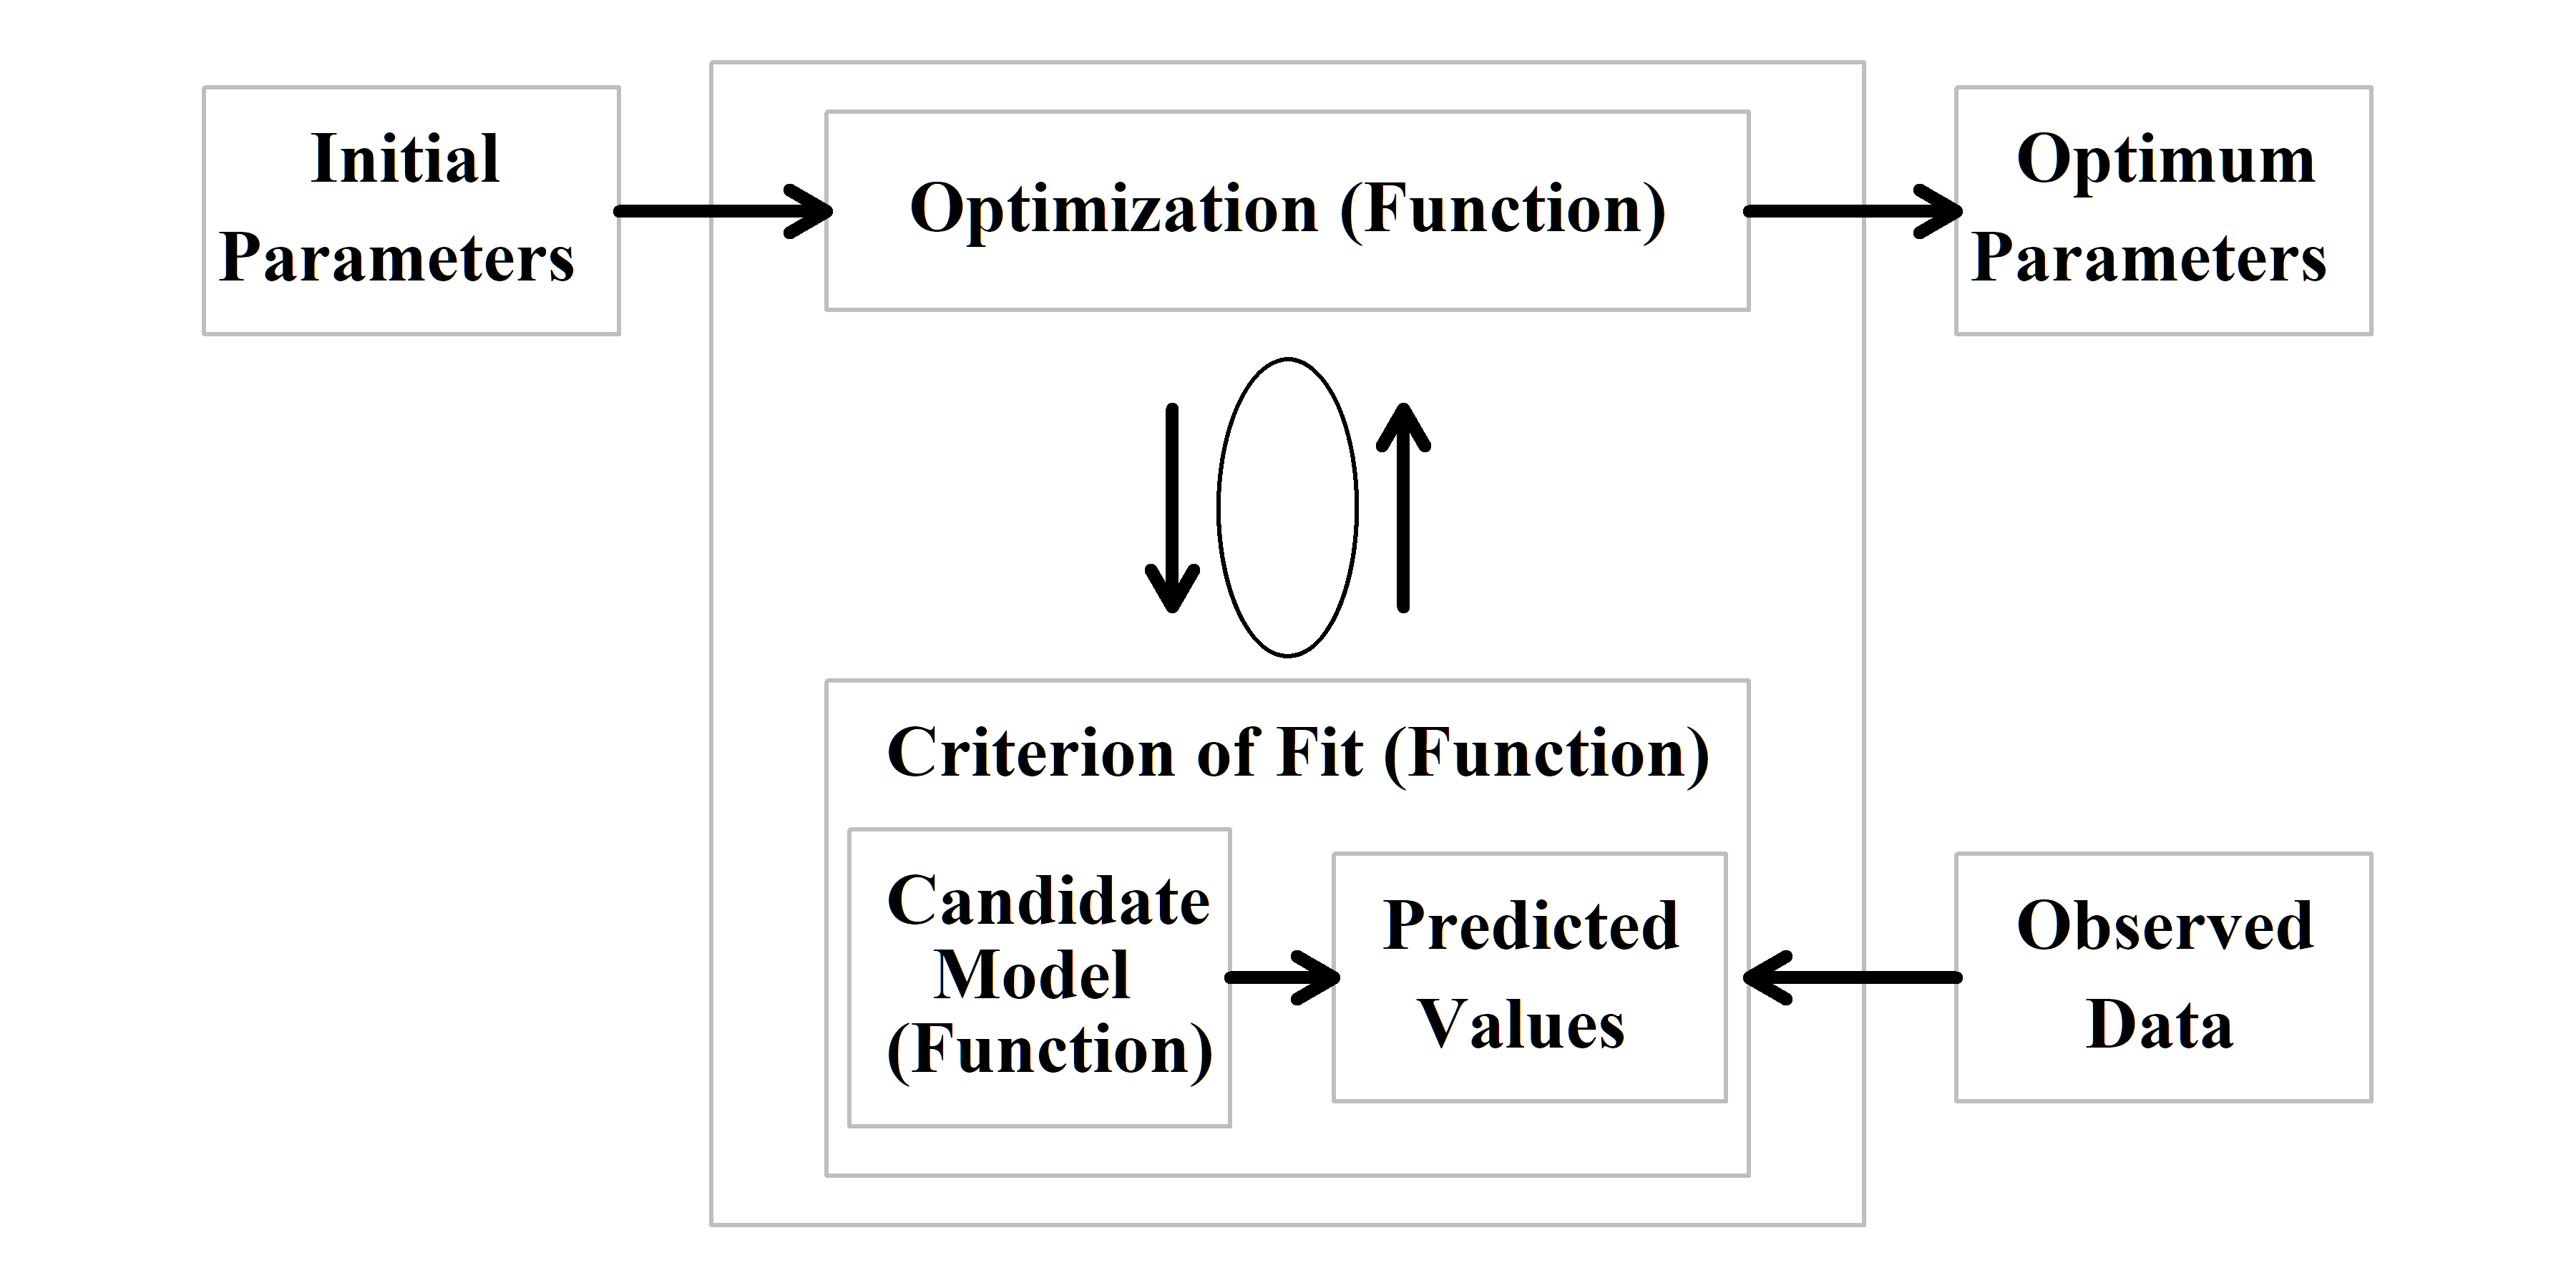
\includegraphics[width=0.5\linewidth]{f401-1} 

}

\caption{Inputs, functional requirements, and outputs, when fitting a model to data. The optimization function (here nlm()) minimizes the negative log-likelihood (or sum-of squares) and requires an initial parameter vector to begin. In addition, the optimizer requires a function (perhaps negLL()) to calculate the corresponding negative log-likelihood for each vector of parameters it produces in its search for the minimum. To calculate the negative log-likelihood requires a function (perhaps vB()) to generate predicted values for comparison with the input observed values.}\label{fig:fig41}
\end{figure}

\subsection{年龄-体长例子}\label{ux5e74ux9f84-ux4f53ux957fux4f8bux5b50}

将模型拟合到数据仅仅意味着估计模型的参数,以便其预测与观测结果相匹配,以及根据选择的最佳拟合标准。作为在 R 中将模型拟合到数据的第一个说明,我们将使用一个简单的示例用著名的 von Bertalanffy 增长曲线 (von Bertalanffy, 1938) 拟合一组年龄-长度数据。这样的数据集包含在 R 包 \textbf{MQMF}(尝试 \texttt{?LatA})中。要使用您自己的数据,一种选择是生成一个逗号分隔的变量 (csv) 文件,其中包含最少的年龄和长度列,每个列都有一个列名(LatA 仅有年龄和长度列;请参阅其帮助页面)。可以使用 \texttt{laa\ \textless{}-\ read.csv(file="filename.csv",\ header=TRUE)} 将此 csv 文件读入 R中。

von Bertalanffy 长度-年龄生长曲线表示为:

\begin{equation}  
\begin{split}    
& {{\hat{L}}_t}={L_{\infty}}\left( 1-{e^{\left( -K\left( t-{t_0} \right) \right)}} \right) \\    
& {L_t}={L_{\infty}}\left( 1-{e^{\left( -K\left( t-{t_0} \right) \right)}} \right)+\varepsilon  \\    
& {L_t}= {\hat{L}}_t + \varepsilon    
\end{split}   
\label{eq:eq44}   
\end{equation}

其中 \(\hat L_t\) 为年龄 \(t\) 的期望或预测长度,\(L_{\infty}\) 为渐近平均最大长度,\(K\) 为是决定达到最大值的增长率系数,\(t_0\) 为物种长度0时的假设年龄(von Bertalanffy, 1938),一旦我们有了\(L_{\infty}\),\(K\) ,\(t_0\) 的估算值(或假设值),该非线性方程就提供了一种预测不同年龄的年龄-长度的方法。在拟合数据模型时,使用\eqref{eq:eq44}中的下面两个方程,其中\(L_t\) 为观测值,等于预测值加上正态随机离差\(\varepsilon = N(0, \sigma^2)\) ,其中的每个值可能是正的或负的(某一年龄的观测值可能大于或小于期望长度)。最下面的方程实际上是关于决定使用什么剩余误差结构。在本章中,我们将描述生态学和渔业中使用的一系列可供选择的误差结构。它们并非都是可加的,有些是用函数关系而不是常数定义的(如\(\sigma\))。

关于式\eqref{eq:eq44}是非线性的表述是明确的,因为早期估计von Bertalanffy (\texttt{vB()})生长曲线参数值的方法涉及各种旨在近似线性化曲线的变换(例如Beverton和Holt, 1957)。在20世纪50年代末和60年代,拟合von Bertalanffy 曲线不是一件小事。令人高兴的是,不再需要这样的转换,这样的曲线拟合也变得很简单。

\subsection{其它的生长模型}\label{ux5176ux5b83ux7684ux751fux957fux6a21ux578b}

个体生长的研究文献很多,描述生物体生长的模型多种多样(Schnute and Richards, 1990)。自Beverton和Holt(1957)引入以来,von Bertalanffy (\texttt{vB()})曲线一直是主要的渔业模型,已被渔业科学家广泛应用。然而,只是因为该模型非常普遍命令使用,对于所有物种来说,并不一定意味着该模型总是提供生长的最佳描述。模型选择是渔业建模中一个至关重要但经常被忽视的方面(Burnham and Anderson, 2002;Helidoniotis and Haddon, 2013)。这里两种替代\texttt{vB()}的两种模型可能是Gompertz生长曲线(Gompertz, 1925):

\begin{equation}
\hat{L_t} =ae^{-be^{ct}} \text{ or } \hat{L_t}=a \exp(-b \exp(ct)) 
\label{eq:eq45}
\end{equation}

以及广义Michaelis-Menten 方程(Maynard Smith and Slatkin, 1973; Legendre and Legendre, 1998):

\begin{equation}  
{{\hat{L}}_{t}}=\frac{at}{b+{{t}^{c}}}  
\label{eq:eq46}  
\end{equation}

每个模型也有 a、b 和 c三个参数,每个模型都能对生长过程的经验数据作出令人信服的描述。可以对某些参数进行生物学解释(如最大平均长度),但这些模型最终只提供了对生长过程的经验描述。如果把模型解释为反映了现实,就会导致完全不可信的预测,如不存在一米长的鱼(Knight,1968 年)。在文献中,参数可以有不同的符号(例如,Maynard Smith 和 Slatkin(1973)用 \(R_0\) 代替 \(a\) 表示 Michaelis-Menton),但基本结构形式是相同的。在对 MQMF 的年龄-长度数据集 \(LatA\) 中的鱼类进行von Bertalanffy生长曲线拟合后,我们可以利用不同模型来说明尝试这些替代模型的价值,并对应该使用哪种模型保持开放的心态。这个问题在我们讨论不确定性时会再次出现,因为我们可以从不同的模型中得到不同的结果。在对任何自然过程建模时,模型选择都是需要做出的重大决定之一。重要的是,通过这种方式尝试不同的模型,还能强化模型与数据拟合的过程。

\section{残差平方和}\label{ux6b8bux5deeux5e73ux65b9ux548c}

数据拟合模型的经典方法称为 ``最小残差平方和''(见式\eqref{eq:eq41} 和式\eqref{eq:eq47}),或更常称为 ``最小二乘法''。这种方法被认为是高斯提出的(Nievergelt, 2000, 引用了高斯 1823 年用拉丁文撰写的一本书的译文:\emph{Theoria combinationis observationum erroribus minimis obnoxiae})。无论如何,最小二乘法符合两个多世纪以来用于确定一组预测值与观测值最佳拟合的策略。这种策略就是确定一个所谓的目标函数(最佳拟合标准),根据函数结构,可以将其最小化或最大化。就残差平方和而言,我们需要从相关的观测值中减去每个预测值,将不同的结果平方(以避免出现负值),然后将所有值相加,并使用数学(解析解)或其他方法将该相加值最小化:

\begin{equation}  
ssq=\sum\limits_{i=1}^{n}{{{\left( {{O}_{i}}-{\hat{E}_{i}} \right)}^{2}}}  
\label{eq:eq47}  
\end{equation}

其中,\(sqq\) 为\emph{n}个观测值的残差平方和,\(O_i\) 为第\(i\) 个观测值,\(E_i\)为第第\(i\) 个观测值的期望值或预测值。\textbf{MQMF}包中的\texttt{ssq} 函数仅仅是一个封装器,它调用了用于生成预测值的任何函数,然后计算并返回平方差和。根据不同问题的复杂程度和数据输入,我们通常需要创建新的函数作为封装。\texttt{ssq()} 很好地说明了这样一个事实,即在一个传递给函数的参数中,也可以传递其他函数(在本例中,在\texttt{ssq()}内我们调用了传递给\texttt{funk} 的函数,当然在使用\texttt{ssq()}时,我们输入的是与当前问题相关的实际函数,也许是\texttt{vB},注意在用作函数参数时没有括号)。

\subsection{最小二乘法的假设}\label{ux6700ux5c0fux4e8cux4e58ux6cd5ux7684ux5047ux8bbe}

最小二乘方法的一个主要假设是,残差项呈正态分布,所有观测变量的方差相等;即在\(\varepsilon = N(0, \sigma^2)\) 中,\(\sigma^2\) 不变。如果以任何方式对数据进行变换,则变换对残差的影响可能违反这一假设。相反,如果残差以系统的方式变化,则转换可以标准化残差。因此,如果数据是对数正态分布,那么对数变换将使数据标准化,然后可以有效地使用最小二乘。与往常一样,考虑或可视化数据和残差的形式(由拟合模型产生)是一种很好的做法。

\subsection{数值求解}\label{ux6570ux503cux6c42ux89e3}

渔业科学中大多数有趣的问题都没有解析解(如线性回归),有必要使用数值方法通过定义的''最佳拟合''标准(如最小残差平方和(最小二乘))来寻找最佳拟合模型。这显然会涉及到一点R编程,但是R的一个很大的优势是,一旦你开发了一套分析方法,就可以直接地将其应用到新的数据集。

在下面的示例中,我们用\textbf{MQMF}中的一些实用函数来辅助描述。我们需要5个函数拟合和比较上文定义的3种不同的生长模型,其中4个需要编写。前3个函数用于估计与观测数据进行比较的各年龄长度预测值。本例有3个候选模型函数分别对应3种不同的生长曲线:\texttt{vB()}、\texttt{Gz()}和\texttt{mm()}。第4个函数用作计算预测值及其相关观测值的平方和残差。这里将使用\textbf{MQMF}中的函数\texttt{ssq()}(你应该检查并理解其代码)。该函数返回单一数值,该值将由最后一个函数\texttt{nlm()}最小化,该函数需要自动最小化求解。R函数\texttt{nlm()}使用用户定义的通用函数,用 \(f\) 表示 (尝试\texttt{args(nlm)},或\texttt{formals(nlm)}以查看完整的参数列表),用于计算最小值(在本例中为\texttt{ssq()}),而\texttt{ssq()}又使用预测生长曲线中各年龄长度的函数(例如\texttt{vB()})。如果我们使用不同的生长曲线函数(例如\texttt{Gz()}),只需将\texttt{nlm()}调用代码中指向\texttt{vB()的地方改为Gz()},并修改参数值以适应\texttt{Gz()}函数,以便代码产生可用的结果。从根本上说,\texttt{nlm()}通过改变输入参数(称作\emph{p})来最小化\texttt{ssq()},无论选择哪个参数,都会改变生长函数\texttt{vB()}、\texttt{Gz()}或\texttt{mm()}的结果,。

\texttt{nlm()}只是\textbf{R}中用于非线性优化的函数之一,候选函数包括\texttt{optim()}和\texttt{nlminb()}(请阅读\texttt{nlm}中的文档,CRAN上关于优化的任务视图列出了旨在解决优化问题的包)。

\begin{Shaded}
\begin{Highlighting}[]
\FunctionTok{library}\NormalTok{(MQMF)}
\FunctionTok{library}\NormalTok{(ggplot2)}
\end{Highlighting}
\end{Shaded}

\begin{verbatim}
## Warning: package 'ggplot2' was built under R version 4.4.3
\end{verbatim}

\begin{Shaded}
\begin{Highlighting}[]
 \CommentTok{\#setup optimization using growth and ssq  }
\FunctionTok{data}\NormalTok{(LatA)      }\CommentTok{\# try ?LatA   assumes library(MQMF) already run  }
 \CommentTok{\#convert equations 4.4 to 4.6 into vectorized R functions  }
 \CommentTok{\#These will over{-}write the same functions in the MQMF package  }
\NormalTok{vB }\OtherTok{\textless{}{-}} \ControlFlowTok{function}\NormalTok{(p, ages) }\FunctionTok{return}\NormalTok{(p[}\DecValTok{1}\NormalTok{]}\SpecialCharTok{*}\NormalTok{(}\DecValTok{1}\SpecialCharTok{{-}}\FunctionTok{exp}\NormalTok{(}\SpecialCharTok{{-}}\NormalTok{p[}\DecValTok{2}\NormalTok{]}\SpecialCharTok{*}\NormalTok{(ages}\SpecialCharTok{{-}}\NormalTok{p[}\DecValTok{3}\NormalTok{]))))  }
\NormalTok{Gz }\OtherTok{\textless{}{-}} \ControlFlowTok{function}\NormalTok{(p, ages) }\FunctionTok{return}\NormalTok{(p[}\DecValTok{1}\NormalTok{]}\SpecialCharTok{*}\FunctionTok{exp}\NormalTok{(}\SpecialCharTok{{-}}\NormalTok{p[}\DecValTok{2}\NormalTok{]}\SpecialCharTok{*}\FunctionTok{exp}\NormalTok{(p[}\DecValTok{3}\NormalTok{]}\SpecialCharTok{*}\NormalTok{ages)))  }
\NormalTok{mm }\OtherTok{\textless{}{-}} \ControlFlowTok{function}\NormalTok{(p, ages) }\FunctionTok{return}\NormalTok{((p[}\DecValTok{1}\NormalTok{]}\SpecialCharTok{*}\NormalTok{ages)}\SpecialCharTok{/}\NormalTok{(p[}\DecValTok{2}\NormalTok{] }\SpecialCharTok{+}\NormalTok{ ages}\SpecialCharTok{\^{}}\NormalTok{p[}\DecValTok{3}\NormalTok{]))  }
 \CommentTok{\#specific function to calc ssq. The ssq within MQMF is more  }
\NormalTok{ssq }\OtherTok{\textless{}{-}} \ControlFlowTok{function}\NormalTok{(p,funk,agedata,observed) \{        }\CommentTok{\#general and is  }
\NormalTok{  predval }\OtherTok{\textless{}{-}} \FunctionTok{funk}\NormalTok{(p,agedata)        }\CommentTok{\#not limited to p and agedata  }
  \FunctionTok{return}\NormalTok{(}\FunctionTok{sum}\NormalTok{((observed }\SpecialCharTok{{-}}\NormalTok{ predval)}\SpecialCharTok{\^{}}\DecValTok{2}\NormalTok{,}\AttributeTok{na.rm=}\ConstantTok{TRUE}\NormalTok{))  }
\NormalTok{\} }\CommentTok{\#end of ssq   }
 \CommentTok{\# guess starting values for Linf, K, and t0, names not needed  }
\NormalTok{pars }\OtherTok{\textless{}{-}} \FunctionTok{c}\NormalTok{(}\StringTok{"Linf"}\OtherTok{=}\FloatTok{27.0}\NormalTok{,}\StringTok{"K"}\OtherTok{=}\FloatTok{0.15}\NormalTok{,}\StringTok{"t0"}\OtherTok{=}\SpecialCharTok{{-}}\FloatTok{2.0}\NormalTok{) }\CommentTok{\#ssq should=1478.449  }
\FunctionTok{ssq}\NormalTok{(}\AttributeTok{p=}\NormalTok{pars, }\AttributeTok{funk=}\NormalTok{vB, }\AttributeTok{agedata=}\NormalTok{LatA}\SpecialCharTok{$}\NormalTok{age, }\AttributeTok{observed=}\NormalTok{LatA}\SpecialCharTok{$}\NormalTok{length)   }
\end{Highlighting}
\end{Shaded}

\begin{verbatim}
## [1] 1478.449
\end{verbatim}

\texttt{ssq()}函数取代了全局环境中的\texttt{MQMF::ssq()}函数,但也返回一个数值,例如上面的1478.449,它是\texttt{nlm()}函数的第一个输入,并且是最小值。

\subsection{将函数作为参数传递给其它函数}\label{ux5c06ux51fdux6570ux4f5cux4e3aux53c2ux6570ux4f20ux9012ux7ed9ux5176ux5b83ux51fdux6570}

在上例中,我们定义了一些用于模型拟合数据所需的函数,确定了要比较的生长模型,也定义了计算平方和的函数。刚刚做的一个非常重要的方面是,为了计算平方和,我们将\texttt{vB()}函数作为参数传递给\texttt{ssq()}函数。这意味着我们传递了一个函数,它有参数,作为另一个函数的参数之一。你可以在这里看到潜在的混乱,所以有必要集中精力,保持清晰。目前,我们定义\texttt{ssq()}的方式似乎并没有那么引人注目,因为我们已经在对\texttt{ssq()}的调用中显式地定义了两个函数的参数。但是R有一些妙招,我们可以用它来泛化包含其他函数作为参数的函数,主要的一个使用了神奇的省略号\texttt{…},对于任何R函数,除非实参在其定义中设置了默认值,否则每个实参都必须给定一个值。在上面的\texttt{ssq()}函数中,我们包含了仅由\texttt{ssq()} 使用的参数(\emph{funk}和\emph{observed}),以及仅由函数\texttt{funk}使用的参数 (\emph{p}和\emph{agedata})。这在本例子中很有效,因为我们故意将生长函数定义为具有相同的输入参数,但如果我们想使用的\texttt{funk}有不同的输入,可能是因为我们拟合的是选择性曲线而不是生长曲线,该怎么办?显然,我们需要编写一个不同的\texttt{ssq()}函数。为了允许在更多情况下重用更通用的函数,R的作者(R Core Team, 2019)包含了这个概念\texttt{…},它将匹配其他方式不匹配的任何参数,因此可用于输入\texttt{funk}函数的参数。因此,我们可以这样重新定义\texttt{ssq()}:

\begin{Shaded}
\begin{Highlighting}[]
 \CommentTok{\# Illustrates use of names within function arguments  }
\NormalTok{vB }\OtherTok{\textless{}{-}} \ControlFlowTok{function}\NormalTok{(p,ages) }\FunctionTok{return}\NormalTok{(p[}\DecValTok{1}\NormalTok{]}\SpecialCharTok{*}\NormalTok{(}\DecValTok{1}\SpecialCharTok{{-}}\FunctionTok{exp}\NormalTok{(}\SpecialCharTok{{-}}\NormalTok{p[}\DecValTok{2}\NormalTok{] }\SpecialCharTok{*}\NormalTok{(ages}\SpecialCharTok{{-}}\NormalTok{p[}\DecValTok{3}\NormalTok{]))))  }
\NormalTok{ssq }\OtherTok{\textless{}{-}} \ControlFlowTok{function}\NormalTok{(funk,observed,...) \{ }\CommentTok{\# only define ssq arguments  }
\NormalTok{  predval }\OtherTok{\textless{}{-}} \FunctionTok{funk}\NormalTok{(...) }\CommentTok{\# funks arguments are implicit  }
  \FunctionTok{return}\NormalTok{(}\FunctionTok{sum}\NormalTok{((observed }\SpecialCharTok{{-}}\NormalTok{ predval)}\SpecialCharTok{\^{}}\DecValTok{2}\NormalTok{,}\AttributeTok{na.rm=}\ConstantTok{TRUE}\NormalTok{))  }
\NormalTok{\} }\CommentTok{\# end of ssq   }
\NormalTok{pars }\OtherTok{\textless{}{-}} \FunctionTok{c}\NormalTok{(}\StringTok{"Linf"}\OtherTok{=}\FloatTok{27.0}\NormalTok{,}\StringTok{"K"}\OtherTok{=}\FloatTok{0.15}\NormalTok{,}\StringTok{"t0"}\OtherTok{=}\SpecialCharTok{{-}}\FloatTok{2.0}\NormalTok{) }\CommentTok{\# ssq should = 1478.449  }
\FunctionTok{ssq}\NormalTok{(}\AttributeTok{p=}\NormalTok{pars, }\AttributeTok{funk=}\NormalTok{vB, }\AttributeTok{ages=}\NormalTok{LatA}\SpecialCharTok{$}\NormalTok{age, }\AttributeTok{observed=}\NormalTok{LatA}\SpecialCharTok{$}\NormalTok{length) }\CommentTok{\#if no  }
\end{Highlighting}
\end{Shaded}

\begin{verbatim}
## [1] 1478.449
\end{verbatim}

\begin{Shaded}
\begin{Highlighting}[]
\FunctionTok{ssq}\NormalTok{(vB,LatA}\SpecialCharTok{$}\NormalTok{length,pars,LatA}\SpecialCharTok{$}\NormalTok{age) }\CommentTok{\# name order is now vital!  }
\end{Highlighting}
\end{Shaded}

\begin{verbatim}
## [1] 1478.449
\end{verbatim}

这意味着\texttt{ssq()}函数现在更加通用,可以与任何输入函数一起使用,这些输入函数可用于生成一组预测值,以便与一组观测值进行比较。\textbf{MQMF}中的\texttt{ssq()}函数就是这样实现的;查阅帮助 \texttt{?ssq}。一般的想法是,您必须定义主函数中使用的所有参数,但任何仅在被调用函数(此处称为\emph{funk})中使用的参数都可以在\texttt{…}中传递。最好是显式地命名参数,这样它们的顺序就无关紧要了,并且您需要非常小心地键入,如果您拼错了通过\texttt{…}传递的参数的名称,并不一定会出错!例如,使用大写的\emph{LatA\$Age}而不是\emph{LatA\$age}不会出错,但会导致结果为0而不是1478.440。这是因为\emph{LatA\$Age = NULL},即使输入不正确也是有效的。很明显,\texttt{…}可能非常有用,但如果你像我一样输入错误,其本身也是有风险的。

\begin{Shaded}
\begin{Highlighting}[]
 \CommentTok{\# Illustrate a problem with calling a function in a function  }
 \CommentTok{\# LatA$age is typed as LatA$Age but no error, and result = 0  }
\FunctionTok{ssq}\NormalTok{(}\AttributeTok{funk=}\NormalTok{vB, }\AttributeTok{observed=}\NormalTok{LatA}\SpecialCharTok{$}\NormalTok{length, }\AttributeTok{p=}\NormalTok{pars, }\AttributeTok{ages=}\NormalTok{LatA}\SpecialCharTok{$}\NormalTok{Age) }\CommentTok{\# !!!  }
\end{Highlighting}
\end{Shaded}

\begin{verbatim}
## [1] 0
\end{verbatim}

如果你匆忙行事,没有给参数命名,那么如果你弄错了参数顺序,也会失败。例如,如果你要输入的是\texttt{ssq(LatA\$length,\ vB,\ pars,\ LatA\$age)}而不是\texttt{ssq(vB,\ LatA\$length,\ pars,\ LatA\$age)},就会出现错误:\emph{Error in funk(\ldots): could not find function '' funk ``}。为了以防万一,你可以自己试试。对你的代码进行试验几乎没什么坏处,不会弄坏你的电脑,而你可能会学到一些东西。

\subsection{拟合模型}\label{ux62dfux5408ux6a21ux578b}

如果我们绘制\emph{LatA}数据集图(图\ref{fig:fig42}),可以看到一些典型的年龄-长度数据。图中有358个点(试试\texttt{dim(LatA)}),许多点彼此重叠,但是当我们使用\texttt{plot()}函数中\texttt{rgb()}选项来改变图中颜色的透明度时,较高年龄组鱼类的颜色相对稀疏性就会显现出来。另外,我们可以使用\texttt{jitter()}为每个绘制点的位置添加噪声,以查看数据点的相对密度。每当你处理经验数据时,总是值得你花时间至少将其绘制成画并探索其属性。

\begin{Shaded}
\begin{Highlighting}[]
 \CommentTok{\#plot the LatA data set   Figure 4.2  }
\FunctionTok{parset}\NormalTok{()        }\CommentTok{\# parset and getmax are two MQMF functions   }
\NormalTok{ymax }\OtherTok{\textless{}{-}} \FunctionTok{getmax}\NormalTok{(LatA}\SpecialCharTok{$}\NormalTok{length) }\CommentTok{\# simplifies use of base graphics. For  }
 \CommentTok{\# full colour, with the rgb as set{-}up below, there must be \textgreater{}= 5 obs  }
\FunctionTok{plot}\NormalTok{(LatA}\SpecialCharTok{$}\NormalTok{age,LatA}\SpecialCharTok{$}\NormalTok{length,}\AttributeTok{type=}\StringTok{"p"}\NormalTok{,}\AttributeTok{pch=}\DecValTok{16}\NormalTok{,}\AttributeTok{cex=}\FloatTok{1.2}\NormalTok{,}\AttributeTok{xlab=}\StringTok{"Age Years"}\NormalTok{,   }
     \AttributeTok{ylab=}\StringTok{"Length cm"}\NormalTok{,}\AttributeTok{col=}\FunctionTok{rgb}\NormalTok{(}\DecValTok{1}\NormalTok{,}\DecValTok{0}\NormalTok{,}\DecValTok{0}\NormalTok{,}\DecValTok{1}\SpecialCharTok{/}\DecValTok{5}\NormalTok{),}\AttributeTok{ylim=}\FunctionTok{c}\NormalTok{(}\DecValTok{0}\NormalTok{,ymax),}\AttributeTok{yaxs=}\StringTok{"i"}\NormalTok{,  }
     \AttributeTok{xlim=}\FunctionTok{c}\NormalTok{(}\DecValTok{0}\NormalTok{,}\DecValTok{44}\NormalTok{),}\AttributeTok{panel.first=}\FunctionTok{grid}\NormalTok{())  }
\end{Highlighting}
\end{Shaded}

\begin{figure}
\centering
\pandocbounded{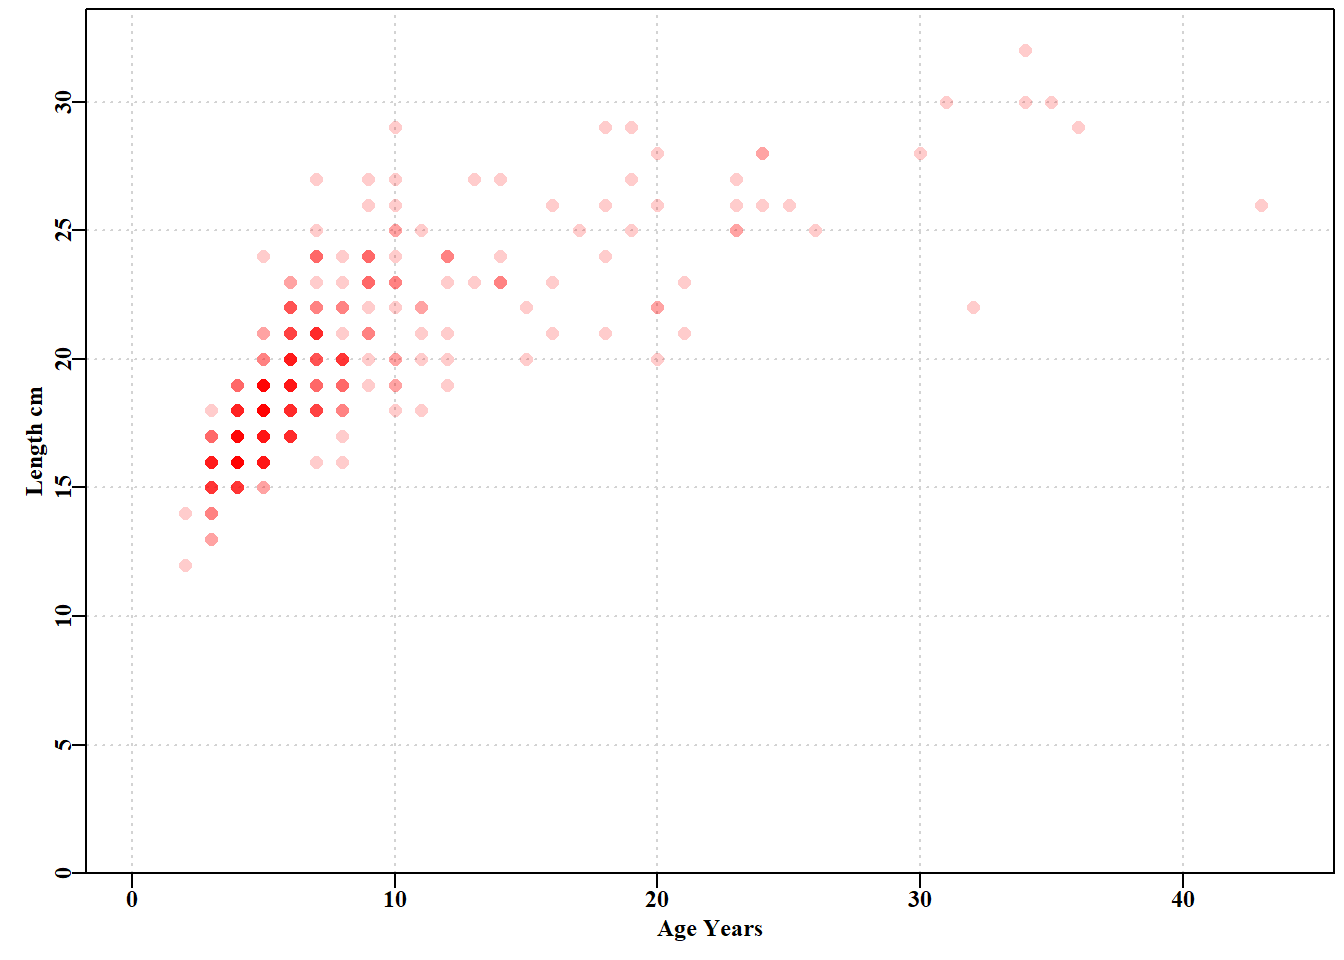
\includegraphics[keepaspectratio]{04-application_files/figure-latex/fig42-1.pdf}}
\caption{\label{fig:fig42}Simulated female length-at-age data for 358 Redfish, Centroberyx affinis, based on samples from eastern Australia. Full intensity colour means \textgreater= 5 points.}
\end{figure}

\begin{Shaded}
\begin{Highlighting}[]
\CommentTok{\# ggplot(data = LatA, aes(x = age, y = length)) +}
\CommentTok{\#   geom\_point(size = 3, color = "red", alpha = 0.2) +}
\CommentTok{\#   labs(x = "Age Years", }
\CommentTok{\#        y = "Length cm") +}
\CommentTok{\#   theme\_bw()}
\end{Highlighting}
\end{Shaded}

与其继续猜测参数值并手动修改它们,我们可以使用\texttt{nlm()}(或\texttt{optim()}或\texttt{nlminb()},它们的语法不同)来拟合所选的\emph{LatA}数据的生长模型或曲线。这不仅说明了\texttt{nlm()}的语法,还说明了另外两个\textbf{MQMF}实用R函数\texttt{magnitude()}和\texttt{outfit()}的使用(请查阅\texttt{?nlm}、\texttt{?magnitude}和\texttt{?outfit})。还可以查看每个函数中的代码(在控制台中输入每个函数的名称,不带参数或括号)。从现在起,我将减少提示你查看所使用函数细节的次数,但是如果看到一个新的函数,希望现查看其帮助、语法,尤其是代码是有意义的,就像查看每个所用变量的内容一样。

3个生长模型中的每一个都需要估计3个参数,我们需要对每个参数进行初始猜测,以启动\texttt{nlm()}求解。我们所做的就是为\texttt{nlm()}函数的每个形参/实参提供值。此外,我们还使用了2个额外的参数,\emph{typsize}和\emph{iterlim}。\emph{typesize}在\texttt{nlm()}帮助中定义为''每个参数最小值的估计''。加入这2个参数一般有助于稳定搜索算法,因为它可以确保对每个参数值迭代变化尺度大致相同。一种非常常见的替代方法(我们将在更复杂的模型中使用)是在输入\texttt{nlm()}时对每个参数进行对数变换,然后在调用的函数中对它们进行反变换,以计算预测值。但是,这只能在保证参数始终为正值情况下才可行。例如,对于von Bertalanffy曲线,\(t_0\) 参数通常是负值,因此应使用\texttt{magnitude()}而不是对数变换方法。默认的\texttt{iterlim=100}意味着最多迭代100次,这有时是不够的,所以如果迭代达到100次,您应该将该数值增加到1000。你很快就会发现,在每次模型拟合过程中,唯一改变的是\texttt{ssq()}中的\emph{funk}所指向的函数和初始参数值。这可以通过有意识地构建生长函数,使其使用完全相同的参数(通过\texttt{…}传递)。您也可以尝试在不设置\emph{typsize}和\emph{interlim}选项的情况下运行其中的一个或两个函数。还请注意,我们运行Michaelis-Menton曲线时使用了两个略有不同的初始点。

\begin{Shaded}
\begin{Highlighting}[]
 \CommentTok{\# use nlm to fit 3 growth curves to LatA, only p and funk change }
\NormalTok{ages }\OtherTok{\textless{}{-}} \DecValTok{1}\SpecialCharTok{:}\FunctionTok{max}\NormalTok{(LatA}\SpecialCharTok{$}\NormalTok{age) }\CommentTok{\# used in comparisons   }
\NormalTok{pars }\OtherTok{\textless{}{-}} \FunctionTok{c}\NormalTok{(}\FloatTok{27.0}\NormalTok{,}\FloatTok{0.15}\NormalTok{,}\SpecialCharTok{{-}}\FloatTok{2.0}\NormalTok{) }\CommentTok{\# von Bertalanffy  }
\NormalTok{bestvB }\OtherTok{\textless{}{-}} \FunctionTok{nlm}\NormalTok{(}\AttributeTok{f=}\NormalTok{ssq,}\AttributeTok{funk=}\NormalTok{vB,}\AttributeTok{observed=}\NormalTok{LatA}\SpecialCharTok{$}\NormalTok{length,}\AttributeTok{p=}\NormalTok{pars,  }
             \AttributeTok{ages=}\NormalTok{LatA}\SpecialCharTok{$}\NormalTok{age,}\AttributeTok{typsize=}\FunctionTok{magnitude}\NormalTok{(pars))  }
\FunctionTok{outfit}\NormalTok{(bestvB,}\AttributeTok{backtran=}\ConstantTok{FALSE}\NormalTok{,}\AttributeTok{title=}\StringTok{"vB"}\NormalTok{); }\FunctionTok{cat}\NormalTok{(}\StringTok{"}\SpecialCharTok{\textbackslash{}n}\StringTok{"}\NormalTok{)   }
\end{Highlighting}
\end{Shaded}

\begin{verbatim}
## nlm solution:  vB 
## minimum     :  1361.421 
## iterations  :  24 
## code        :  2 >1 iterates in tolerance, probably solution 
##          par      gradient
## 1 26.8353971 -1.133124e-04
## 2  0.1301587 -6.189993e-03
## 3 -3.5866989  8.319266e-05
\end{verbatim}

\begin{Shaded}
\begin{Highlighting}[]
\NormalTok{pars }\OtherTok{\textless{}{-}} \FunctionTok{c}\NormalTok{(}\FloatTok{26.0}\NormalTok{,}\FloatTok{0.7}\NormalTok{,}\SpecialCharTok{{-}}\FloatTok{0.5}\NormalTok{) }\CommentTok{\# Gompertz  }
\NormalTok{bestGz }\OtherTok{\textless{}{-}} \FunctionTok{nlm}\NormalTok{(}\AttributeTok{f=}\NormalTok{ssq,}\AttributeTok{funk=}\NormalTok{Gz,}\AttributeTok{observed=}\NormalTok{LatA}\SpecialCharTok{$}\NormalTok{length,}\AttributeTok{p=}\NormalTok{pars,  }
             \AttributeTok{ages=}\NormalTok{LatA}\SpecialCharTok{$}\NormalTok{age,}\AttributeTok{typsize=}\FunctionTok{magnitude}\NormalTok{(pars))  }
\FunctionTok{outfit}\NormalTok{(bestGz,}\AttributeTok{backtran=}\ConstantTok{FALSE}\NormalTok{,}\AttributeTok{title=}\StringTok{"Gz"}\NormalTok{); }\FunctionTok{cat}\NormalTok{(}\StringTok{"}\SpecialCharTok{\textbackslash{}n}\StringTok{"}\NormalTok{)   }
\end{Highlighting}
\end{Shaded}

\begin{verbatim}
## nlm solution:  Gz 
## minimum     :  1374.36 
## iterations  :  28 
## code        :  1 gradient close to 0, probably solution 
##          par      gradient
## 1 26.4444554  2.725617e-05
## 2  0.8682518 -6.447369e-04
## 3 -0.1635476 -2.043683e-03
\end{verbatim}

\begin{Shaded}
\begin{Highlighting}[]
\NormalTok{pars }\OtherTok{\textless{}{-}} \FunctionTok{c}\NormalTok{(}\FloatTok{26.2}\NormalTok{,}\FloatTok{1.0}\NormalTok{,}\FloatTok{1.0}\NormalTok{) }\CommentTok{\# Michaelis{-}Menton {-} first start point  }
\NormalTok{bestMM1 }\OtherTok{\textless{}{-}} \FunctionTok{nlm}\NormalTok{(}\AttributeTok{f=}\NormalTok{ssq,}\AttributeTok{funk=}\NormalTok{mm,}\AttributeTok{observed=}\NormalTok{LatA}\SpecialCharTok{$}\NormalTok{length,}\AttributeTok{p=}\NormalTok{pars,  }
             \AttributeTok{ages=}\NormalTok{LatA}\SpecialCharTok{$}\NormalTok{age,}\AttributeTok{typsize=}\FunctionTok{magnitude}\NormalTok{(pars))  }
\FunctionTok{outfit}\NormalTok{(bestMM1,}\AttributeTok{backtran=}\ConstantTok{FALSE}\NormalTok{,}\AttributeTok{title=}\StringTok{"MM"}\NormalTok{); }\FunctionTok{cat}\NormalTok{(}\StringTok{"}\SpecialCharTok{\textbackslash{}n}\StringTok{"}\NormalTok{)  }
\end{Highlighting}
\end{Shaded}

\begin{verbatim}
## nlm solution:  MM 
## minimum     :  1335.961 
## iterations  :  12 
## code        :  2 >1 iterates in tolerance, probably solution 
##          par    gradient
## 1 20.6633224 -0.02622726
## 2  1.4035207 -0.37744299
## 3  0.9018319 -0.05039283
\end{verbatim}

\begin{Shaded}
\begin{Highlighting}[]
\NormalTok{pars }\OtherTok{\textless{}{-}} \FunctionTok{c}\NormalTok{(}\FloatTok{23.0}\NormalTok{,}\FloatTok{1.0}\NormalTok{,}\FloatTok{1.0}\NormalTok{) }\CommentTok{\# Michaelis{-}Menton {-} second start point  }
\NormalTok{bestMM2 }\OtherTok{\textless{}{-}} \FunctionTok{nlm}\NormalTok{(}\AttributeTok{f=}\NormalTok{ssq,}\AttributeTok{funk=}\NormalTok{mm,}\AttributeTok{observed=}\NormalTok{LatA}\SpecialCharTok{$}\NormalTok{length,}\AttributeTok{p=}\NormalTok{pars,  }
             \AttributeTok{ages=}\NormalTok{LatA}\SpecialCharTok{$}\NormalTok{age,}\AttributeTok{typsize=}\FunctionTok{magnitude}\NormalTok{(pars))  }
\FunctionTok{outfit}\NormalTok{(bestMM2,}\AttributeTok{backtran=}\ConstantTok{FALSE}\NormalTok{,}\AttributeTok{title=}\StringTok{"MM2"}\NormalTok{); }\FunctionTok{cat}\NormalTok{(}\StringTok{"}\SpecialCharTok{\textbackslash{}n}\StringTok{"}\NormalTok{)   }
\end{Highlighting}
\end{Shaded}

\begin{verbatim}
## nlm solution:  MM2 
## minimum     :  1335.957 
## iterations  :  25 
## code        :  1 gradient close to 0, probably solution 
##          par      gradient
## 1 20.7464274  8.466004e-06
## 2  1.4183164 -3.856475e-05
## 3  0.9029899 -1.297462e-04
\end{verbatim}

这些都是数值解,它们不能保证是正确的解。请注意,第一个Michaelis-Menton解(从26.2,1,1开始)的梯度相对较大,但它的SSQ(1335.96)非常接近第二个Michaelis-Menton模型拟合,而且比vB或Gz曲线更小(更好)。然而,梯度值表明该模型的拟合可以而且应该得到改进。如果您将参数\emph{a}(首个MM参数)的初始参数估计值从上次模型拟合中的26.2降到了23,我们就会得到稍有不同的参数值、稍小的SSQ以及更小的梯度,从而更有把握地认为结果是个真正的最小值。实际上,如果要运行\texttt{cbind(mm(bestMM1\$estimate,ages),\ mm(bestMM2\$estimate,ages))},可以计算出预测值的差异从-0.018到0.21\%,而如果将vB预测值包括在内,MM2与vB预测的差异从-6.15到9.88\%(忽略40.6\%的最大偏差)。你也可以尝试从vB模型的估计中省略\emph{typsize}参数,这样仍然会得到最佳结果,但可查看梯度以了解为什么使用\emph{typsize}有助于优化。在设置这些示例时,偶尔运行\texttt{Gz()}模型会出现\emph{steptol}可能太小的注释,将其从默认的1e-06改为1e-05可以很快解决这个问题。如果您遇到了这种情况,请在\texttt{nlm()}命令中添加一条语句\texttt{steptol=1e-05},看看诊断是否有所改善。

显而易见的结论是,我们应该经常查阅\texttt{nlm()}的诊断注释,考虑得到的解的方案的梯度,并且使用多组初始参数猜测,以确保得到稳定的解。数值求解以软件实现为基础,用于决定何时停止迭代的规则有时会被次优解所欺骗。我们的目标是找到全局最小值,而不是局部最小值。任何非线性模型都可能产生此类次优解,因此自动拟合此类模型并非易事。在这种情况下,永远不要假设在这种情况下你得到的第一个答案一定是你正在寻找的最佳答案,即使描绘的模型拟合看起来是可以接受的。

在函数调用中,如果你为每个参数命名,那么严格来讲,顺序并不重要,但我发现一致的用法可以简化代码的阅读,因此即使使用显式名称,也建议使用标准顺序。如果我们不使用显式名称,则\texttt{nlm()}的语法要求首先定义函数最小化(\emph{f})。此外,它还要求\emph{f}函数,无论它是什么,在\emph{p}参数中使用初始参数猜测,如果未命名,则必须排在第二位。如果你在控制台中输入\texttt{formals(nlm)}或\texttt{args(nlm)},就可得到可以输入到函数的可能参数以及它们的默认值(如果存在):

\begin{Shaded}
\begin{Highlighting}[]
 \CommentTok{\#The use of args() and formals()   }
\FunctionTok{args}\NormalTok{(nlm) }\CommentTok{\# formals(nlm) uses more screen space. Try yourself.  }
\end{Highlighting}
\end{Shaded}

\begin{verbatim}
## function (f, p, ..., hessian = FALSE, typsize = rep(1, length(p)), 
##     fscale = 1, print.level = 0, ndigit = 12, gradtol = 1e-06, 
##     stepmax = max(1000 * sqrt(sum((p/typsize)^2)), 1000), steptol = 1e-06, 
##     iterlim = 100, check.analyticals = TRUE) 
## NULL
\end{verbatim}

正如所见,首先要最小化函数f(在本例中是\texttt{ssq()}),然后是初始参数\emph{p},它必须是\emph{f}所指向的任何函数所需的第一个参数。接着是省略号(三个点),它概括了任何函数\emph{f}的\texttt{nlm()}代码,其后是可能的参数集,所有这些参数都具有默认值。我们修改了\emph{typsize}和\emph{iterm}(有时也修改了\texttt{Gz()} 中的\emph{steptol});请参阅\texttt{nlm()}帮助以获得对每种方法的解释。

在R中,\ldots 实际上指的是所需的任何其他输入,例如函数\emph{f}指向的任何参数(本例中为\texttt{ssq})。如果Et \texttt{?ssq}查看参数或代码或帮助,将会看到所需函数\emph{funk},该函数将用于计算相对于\texttt{ssq()}的下一个所需输入的期望值,为观测值的向量(如\(O_i-E_i\))。请注意,这里没有明确提到\emph{funk}使用的参数,这些参数假定是通过\ldots.传递的。在对\texttt{ssq()}的每次调用中,我们都显式地填充了这些参数,例如\texttt{nlm(f=ssq,funk=Gz,\ observed=LatA\$length,\ p=pars,\ ages=LatA\$age,)}。这样,所有要求都已满足,\texttt{ssq()}就可以开始工作。如果不小心忽略了\texttt{ages=LatA\$age}参数,那么在这种情况下,R会出现如下揭示:\emph{Error in funk(par, independent) : argument ``ages'' is missing, with no default}(我相信你会相信我的,但你自己试试也无妨!)。

就生长曲线模型拟合而言,绘制结果提供了一个直观的比较,说明了三条生长曲线之间的差异(Murrell, 2011)。

\begin{Shaded}
\begin{Highlighting}[]
 \CommentTok{\#Female length{-}at{-}age + 3 growth fitted curves Figure 4.3  }
\NormalTok{predvB }\OtherTok{\textless{}{-}} \FunctionTok{vB}\NormalTok{(bestvB}\SpecialCharTok{$}\NormalTok{estimate,ages) }\CommentTok{\#get optimumpredicted lengths  }
\NormalTok{predGz }\OtherTok{\textless{}{-}} \FunctionTok{Gz}\NormalTok{(bestGz}\SpecialCharTok{$}\NormalTok{estimate,ages) }\CommentTok{\# using the outputs  }
\NormalTok{predmm }\OtherTok{\textless{}{-}} \FunctionTok{mm}\NormalTok{(bestMM2}\SpecialCharTok{$}\NormalTok{estimate,ages) }\CommentTok{\#from the nlm analysis above  }
\NormalTok{ymax }\OtherTok{\textless{}{-}} \FunctionTok{getmax}\NormalTok{(LatA}\SpecialCharTok{$}\NormalTok{length) }\CommentTok{\#try ?getmax or getmax [no brackets]  }
\NormalTok{xmax }\OtherTok{\textless{}{-}} \FunctionTok{getmax}\NormalTok{(LatA}\SpecialCharTok{$}\NormalTok{age)  }\CommentTok{\#there is also a getmin, not used here  }
\FunctionTok{parset}\NormalTok{(}\AttributeTok{font=}\DecValTok{7}\NormalTok{)   }\CommentTok{\# or use parsyn() to prompt for the par syntax  }
\FunctionTok{plot}\NormalTok{(LatA}\SpecialCharTok{$}\NormalTok{age,LatA}\SpecialCharTok{$}\NormalTok{length,}\AttributeTok{type=}\StringTok{"p"}\NormalTok{,}\AttributeTok{pch=}\DecValTok{16}\NormalTok{, }\AttributeTok{col=}\FunctionTok{rgb}\NormalTok{(}\DecValTok{1}\NormalTok{,}\DecValTok{0}\NormalTok{,}\DecValTok{0}\NormalTok{,}\DecValTok{1}\SpecialCharTok{/}\DecValTok{5}\NormalTok{),  }
     \AttributeTok{cex=}\FloatTok{1.2}\NormalTok{,}\AttributeTok{xlim=}\FunctionTok{c}\NormalTok{(}\DecValTok{0}\NormalTok{,xmax),}\AttributeTok{ylim=}\FunctionTok{c}\NormalTok{(}\DecValTok{0}\NormalTok{,ymax),}\AttributeTok{yaxs=}\StringTok{"i"}\NormalTok{,}\AttributeTok{xlab=}\StringTok{"Age"}\NormalTok{,  }
     \AttributeTok{ylab=}\StringTok{"Length (cm)"}\NormalTok{,}\AttributeTok{panel.first=}\FunctionTok{grid}\NormalTok{())  }
\FunctionTok{lines}\NormalTok{(ages,predvB,}\AttributeTok{lwd=}\DecValTok{2}\NormalTok{,}\AttributeTok{col=}\DecValTok{4}\NormalTok{)        }\CommentTok{\# vB    col=4=blue  }
\FunctionTok{lines}\NormalTok{(ages,predGz,}\AttributeTok{lwd=}\DecValTok{2}\NormalTok{,}\AttributeTok{col=}\DecValTok{1}\NormalTok{,}\AttributeTok{lty=}\DecValTok{2}\NormalTok{)  }\CommentTok{\# Gompertz  1=black  }
\FunctionTok{lines}\NormalTok{(ages,predmm,}\AttributeTok{lwd=}\DecValTok{2}\NormalTok{,}\AttributeTok{col=}\DecValTok{3}\NormalTok{,}\AttributeTok{lty=}\DecValTok{3}\NormalTok{)  }\CommentTok{\# MM        3=green  }
 \CommentTok{\#notice the legend function and its syntax.  }
\FunctionTok{legend}\NormalTok{(}\StringTok{"bottomright"}\NormalTok{,}\AttributeTok{cex=}\FloatTok{1.2}\NormalTok{,}\FunctionTok{c}\NormalTok{(}\StringTok{"von Bertalanffy"}\NormalTok{,}\StringTok{"Gompertz"}\NormalTok{,  }
       \StringTok{"Michaelis{-}Menton"}\NormalTok{),}\AttributeTok{col=}\FunctionTok{c}\NormalTok{(}\DecValTok{4}\NormalTok{,}\DecValTok{1}\NormalTok{,}\DecValTok{3}\NormalTok{),}\AttributeTok{lty=}\FunctionTok{c}\NormalTok{(}\DecValTok{1}\NormalTok{,}\DecValTok{2}\NormalTok{,}\DecValTok{3}\NormalTok{),}\AttributeTok{lwd=}\DecValTok{3}\NormalTok{,}\AttributeTok{bty=}\StringTok{"n"}\NormalTok{)  }
\end{Highlighting}
\end{Shaded}

\begin{figure}
\centering
\pandocbounded{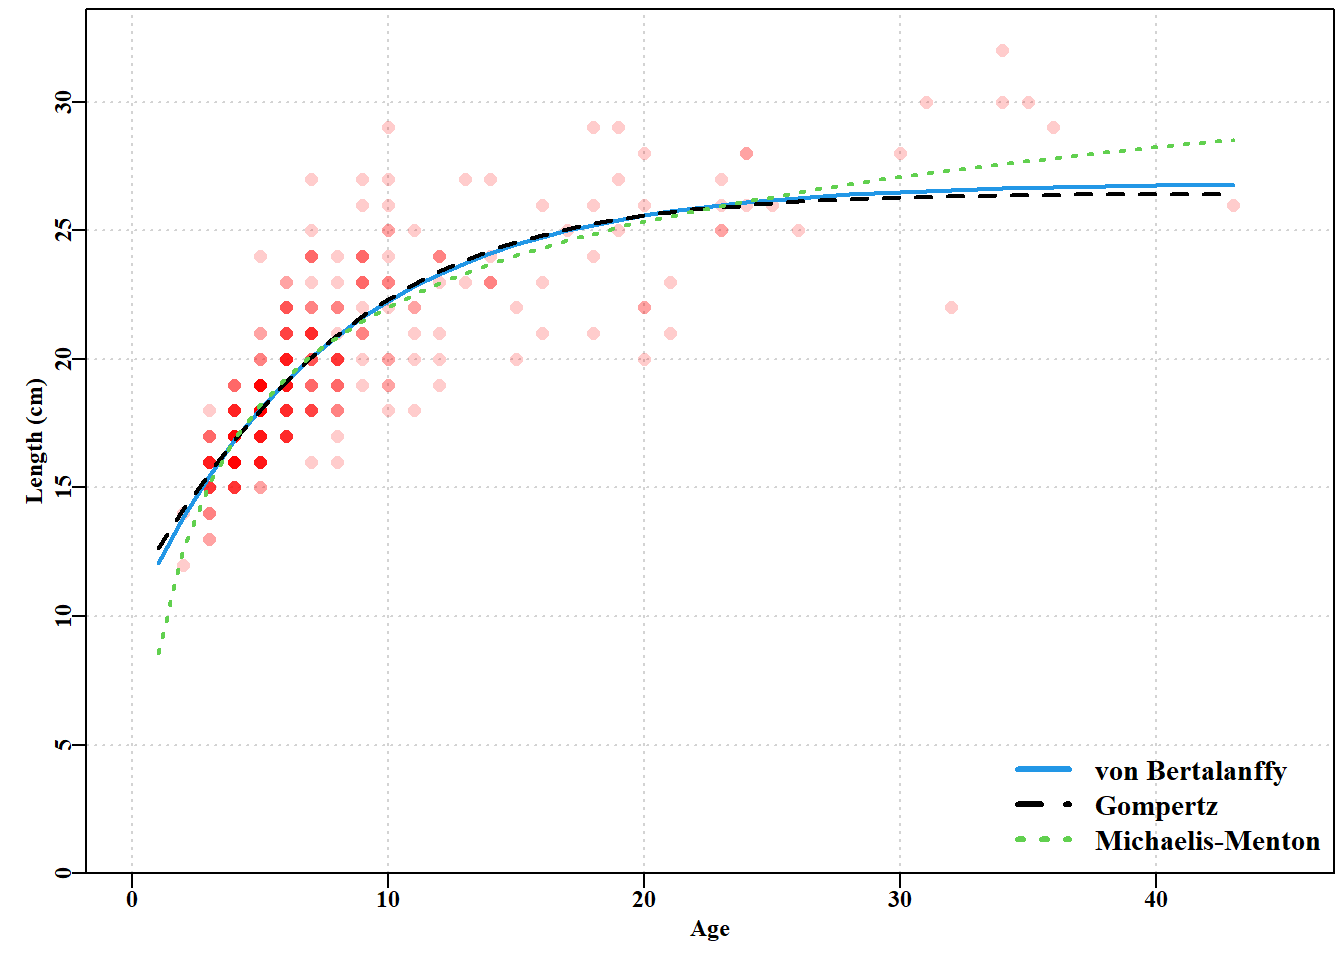
\includegraphics[keepaspectratio]{04-application_files/figure-latex/fig43-1.pdf}}
\caption{\label{fig:fig43}Female Length-at-Age data from 358 simulated female redfish with three optimally fitted growth curves drawn on top.}
\end{figure}

\begin{Shaded}
\begin{Highlighting}[]
\CommentTok{\# ggplot() +}
\CommentTok{\#   geom\_point(data = LatA, aes(x = age, y = length), }
\CommentTok{\#              color = "red", alpha = 0.2) +}
\CommentTok{\#   geom\_line(aes(x = ages, y = predvB), color = "blue") +}
\CommentTok{\#   geom\_line(aes(x = ages, y = predGz), color = "black") +}
\CommentTok{\#   geom\_line(aes(x = ages, y = predmm), color = "green") +}
\CommentTok{\#   theme\_bw()}
\end{Highlighting}
\end{Shaded}

\subsection{目标模型选择}\label{ux76eeux6807ux6a21ux578bux9009ux62e9}

在上述三种生长模型中,最优模型拟合定义为使预测值与实测值之间的平方和残差最小。根据这一标准,第二个生长模型Michaelis-Menton曲线比von Bertalanffy曲线和Gompertz曲线更适合。但我们真的能说第二条米切里斯-门通曲线比第一条曲线''更好''拟合吗?就最终溶液的梯度而言,第二条曲线显然更好,但严格的拟合标准只是最小SSQ,差异小于0.01个单位。模型选择通常是使用参数的数量和根据所选标准的拟合质量之间的权衡。如果我们设计一个具有更多参数的模型,这通常会导致更大的灵活性和更接近观测数据的改进能力。在极端情况下,如果我们有和观测值一样多的参数,我们可以有一个完美的模型拟合,但是,当然,我们对我们正在建模的系统一无所知。LatA数据集有358个参数,这显然是过度参数化的情况,但如果我们只将参数数量增加到10个呢?毫无疑问,曲线的形状会很奇怪,但SSQ可能会更低。Burnham和Anderson(2002)详细讨论了参数数量和模型与数据的拟合质量之间的权衡关系。在20世纪70年代,人们开始使用信息论来开发一种量化模型参数和模型拟合质量之间权衡的方法。Akaike(1974)描述了他的Akaike信息标准(AIC),该标准基于最大似然和信息理论原理(稍后会详细介绍),但幸运的是,Burnham和Anderson(2002)在使用最小平方和残差时提供了另一种选择,这是Atkinson(1980)中包含的一种变体:

\begin{equation}  
AIC=N \left(log\left(\hat\sigma^2 \right) \right)+2p  
\label{eq:eq48}  
\end{equation}

其中\(N\) 为观测数,\(p\) 为''模型内独立调整参数数量''(Akaike,1974,p716),\(\hat{\sigma}^2\) 为方差的最大似然估计,仅表示残差平方和除以\(N\) 而非 \(N-1\) :

\begin{equation}  
\hat\sigma^2 = \frac{\Sigma\varepsilon^2}{N} = \frac{ssq}{N}  
\label{eq:eq49}  
\end{equation}

即使有了\emph{AIC},也很难确定,当使用最小二乘时,差异是否可以被认为是统计上显著的差异。有与方差分析相关的方法,但当使用最大似然时,这些问题能够得到更可靠的回答,所以我们将在后面的部分中解决这个问题。

如果想在拟合模型时获得生物学上合理的或可站得住脚的解释,那么模型选择不能仅仅依赖于统计拟合的质量。相反,它应该反映理论预期(例如,种群中的平均生长是否包括随着时间的推移个体大小的平稳增长,等等)。除了数据的统计拟合之外,这些考虑因素似乎没有得到足够的重视,但只有在出现生物学上不可信的模型结果或提出不可信的模型结构时才变得重要。它显然有助于理解正在建模的过程的生物学期望。

\subsection{残差选择对模型拟合的影响}\label{ux6b8bux5deeux9009ux62e9ux5bf9ux6a21ux578bux62dfux5408ux7684ux5f71ux54cd}

在生长模型例子中,我们使用了正态随机偏差,但我们可以问,如果我们使用,例如对数正态偏差,我们是否会得到相同的答案?在这种情况下,我们所需要做的就是在计算残差平方和之前对观测值和预测值进行对数变换(参见下面关于对数正态残差的内容)。

\begin{equation}  
ssq=\sum\limits_{i=1}^{n}{{{\left( log({O_i})- log({\hat{E_i}}) \right)}^{2}}}  
\label{eq:eq410}  
\end{equation}

这里我们继续在\texttt{outfit()}中使用\emph{backtran=FALSE}选项,因为我们是对数据进行对数转换,而不是对参数进行对数转换,因此不需要进行反向转换。

\begin{Shaded}
\begin{Highlighting}[]
 \CommentTok{\# von Bertalanffy   }
\NormalTok{pars }\OtherTok{\textless{}{-}} \FunctionTok{c}\NormalTok{(}\FloatTok{27.25}\NormalTok{,}\FloatTok{0.15}\NormalTok{,}\SpecialCharTok{{-}}\FloatTok{3.0}\NormalTok{)  }
\NormalTok{bestvBN }\OtherTok{\textless{}{-}} \FunctionTok{nlm}\NormalTok{(}\AttributeTok{f=}\NormalTok{ssq,}\AttributeTok{funk=}\NormalTok{vB,}\AttributeTok{observed=}\NormalTok{LatA}\SpecialCharTok{$}\NormalTok{length,}\AttributeTok{p=}\NormalTok{pars,  }
             \AttributeTok{ages=}\NormalTok{LatA}\SpecialCharTok{$}\NormalTok{age,}\AttributeTok{typsize=}\FunctionTok{magnitude}\NormalTok{(pars),}\AttributeTok{iterlim=}\DecValTok{1000}\NormalTok{)  }
\FunctionTok{outfit}\NormalTok{(bestvBN,}\AttributeTok{backtran=}\ConstantTok{FALSE}\NormalTok{,}\AttributeTok{title=}\StringTok{"Normal errors"}\NormalTok{); }\FunctionTok{cat}\NormalTok{(}\StringTok{"}\SpecialCharTok{\textbackslash{}n}\StringTok{"}\NormalTok{)   }
\end{Highlighting}
\end{Shaded}

\begin{verbatim}
## nlm solution:  Normal errors 
## minimum     :  1361.421 
## iterations  :  22 
## code        :  1 gradient close to 0, probably solution 
##          par      gradient
## 1 26.8353990 -3.650549e-07
## 2  0.1301587 -1.576574e-05
## 3 -3.5867005  3.210883e-07
\end{verbatim}

\begin{Shaded}
\begin{Highlighting}[]
 \CommentTok{\# modify ssq to account for log{-}normal errors in ssqL  }
\NormalTok{ssqL }\OtherTok{\textless{}{-}} \ControlFlowTok{function}\NormalTok{(funk,observed,...) \{  }
\NormalTok{  predval }\OtherTok{\textless{}{-}} \FunctionTok{funk}\NormalTok{(...)  }
  \FunctionTok{return}\NormalTok{(}\FunctionTok{sum}\NormalTok{((}\FunctionTok{log}\NormalTok{(observed) }\SpecialCharTok{{-}} \FunctionTok{log}\NormalTok{(predval))}\SpecialCharTok{\^{}}\DecValTok{2}\NormalTok{,}\AttributeTok{na.rm=}\ConstantTok{TRUE}\NormalTok{))  }
\NormalTok{\} }\CommentTok{\# end of ssqL  }
\NormalTok{bestvBLN }\OtherTok{\textless{}{-}} \FunctionTok{nlm}\NormalTok{(}\AttributeTok{f=}\NormalTok{ssqL,}\AttributeTok{funk=}\NormalTok{vB,}\AttributeTok{observed=}\NormalTok{LatA}\SpecialCharTok{$}\NormalTok{length,}\AttributeTok{p=}\NormalTok{pars,  }
             \AttributeTok{ages=}\NormalTok{LatA}\SpecialCharTok{$}\NormalTok{age,}\AttributeTok{typsize=}\FunctionTok{magnitude}\NormalTok{(pars),}\AttributeTok{iterlim=}\DecValTok{1000}\NormalTok{)  }
\FunctionTok{outfit}\NormalTok{(bestvBLN,}\AttributeTok{backtran=}\ConstantTok{FALSE}\NormalTok{,}\AttributeTok{title=}\StringTok{"Log{-}Normal errors"}\NormalTok{)  }
\end{Highlighting}
\end{Shaded}

\begin{verbatim}
## nlm solution:  Log-Normal errors 
## minimum     :  3.153052 
## iterations  :  25 
## code        :  1 gradient close to 0, probably solution 
##          par      gradient
## 1 26.4409587  8.903296e-08
## 2  0.1375784  7.543602e-06
## 3 -3.2946086 -1.125519e-07
\end{verbatim}

在这种情况下,使用正态和对数正态残差产生的曲线几乎没有区别(图\ref{fig:fig44})。尽管它们的参数不同(使用ylim=c(10,ymax)使差异更清楚)。除了视觉上的不同,不同的模型甚至没有可比性。如果我们比较它们各自的平方和残差,一个有1361.0,另一个只有3.153。当我们考虑到平方和计算中对数变换的影响时,这并不奇怪。但这意味着我们不能只看表格输出,然后决定哪个版本比另一个更适合数据。它们是严格不相称的,尽管它们使用的是完全相同的模型。不同残差结构的使用需要在考虑相对模型拟合以外的方式进行辩护。这个例子强调,虽然模型的选择显然很重要,但残差结构的选择也是模型结构的一部分,同样重要。

\begin{Shaded}
\begin{Highlighting}[]
 \CommentTok{\# Now plot the resultibng two curves and the data Fig 4.4  }
\NormalTok{predvBN }\OtherTok{\textless{}{-}} \FunctionTok{vB}\NormalTok{(bestvBN}\SpecialCharTok{$}\NormalTok{estimate,ages)   }
\NormalTok{predvBLN }\OtherTok{\textless{}{-}} \FunctionTok{vB}\NormalTok{(bestvBLN}\SpecialCharTok{$}\NormalTok{estimate,ages)   }
\NormalTok{ymax }\OtherTok{\textless{}{-}} \FunctionTok{getmax}\NormalTok{(LatA}\SpecialCharTok{$}\NormalTok{length)   }
\NormalTok{xmax }\OtherTok{\textless{}{-}} \FunctionTok{getmax}\NormalTok{(LatA}\SpecialCharTok{$}\NormalTok{age)      }
\FunctionTok{parset}\NormalTok{()                }
\FunctionTok{plot}\NormalTok{(LatA}\SpecialCharTok{$}\NormalTok{age,LatA}\SpecialCharTok{$}\NormalTok{length,}\AttributeTok{type=}\StringTok{"p"}\NormalTok{,}\AttributeTok{pch=}\DecValTok{16}\NormalTok{, }\AttributeTok{col=}\FunctionTok{rgb}\NormalTok{(}\DecValTok{1}\NormalTok{,}\DecValTok{0}\NormalTok{,}\DecValTok{0}\NormalTok{,}\DecValTok{1}\SpecialCharTok{/}\DecValTok{5}\NormalTok{),  }
     \AttributeTok{cex=}\FloatTok{1.2}\NormalTok{,}\AttributeTok{xlim=}\FunctionTok{c}\NormalTok{(}\DecValTok{0}\NormalTok{,xmax),}\AttributeTok{ylim=}\FunctionTok{c}\NormalTok{(}\DecValTok{0}\NormalTok{,ymax),}\AttributeTok{yaxs=}\StringTok{"i"}\NormalTok{,}\AttributeTok{xlab=}\StringTok{"Age"}\NormalTok{,  }
     \AttributeTok{ylab=}\StringTok{"Length (cm)"}\NormalTok{,}\AttributeTok{panel.first=}\FunctionTok{grid}\NormalTok{())  }
\FunctionTok{lines}\NormalTok{(ages,predvBN,}\AttributeTok{lwd=}\DecValTok{2}\NormalTok{,}\AttributeTok{col=}\DecValTok{4}\NormalTok{,}\AttributeTok{lty=}\DecValTok{2}\NormalTok{)   }\CommentTok{\# add Normal dashed  }
\FunctionTok{lines}\NormalTok{(ages,predvBLN,}\AttributeTok{lwd=}\DecValTok{2}\NormalTok{,}\AttributeTok{col=}\DecValTok{1}\NormalTok{)        }\CommentTok{\# add Log{-}Normal solid  }
\FunctionTok{legend}\NormalTok{(}\StringTok{"bottomright"}\NormalTok{,}\FunctionTok{c}\NormalTok{(}\StringTok{"Normal Errors"}\NormalTok{,}\StringTok{"Log{-}Normal Errors"}\NormalTok{),  }
       \AttributeTok{col=}\FunctionTok{c}\NormalTok{(}\DecValTok{4}\NormalTok{,}\DecValTok{1}\NormalTok{),}\AttributeTok{lty=}\FunctionTok{c}\NormalTok{(}\DecValTok{2}\NormalTok{,}\DecValTok{1}\NormalTok{),}\AttributeTok{lwd=}\DecValTok{3}\NormalTok{,}\AttributeTok{bty=}\StringTok{"n"}\NormalTok{,}\AttributeTok{cex=}\FloatTok{1.2}\NormalTok{)  }
\end{Highlighting}
\end{Shaded}

\begin{figure}
\centering
\pandocbounded{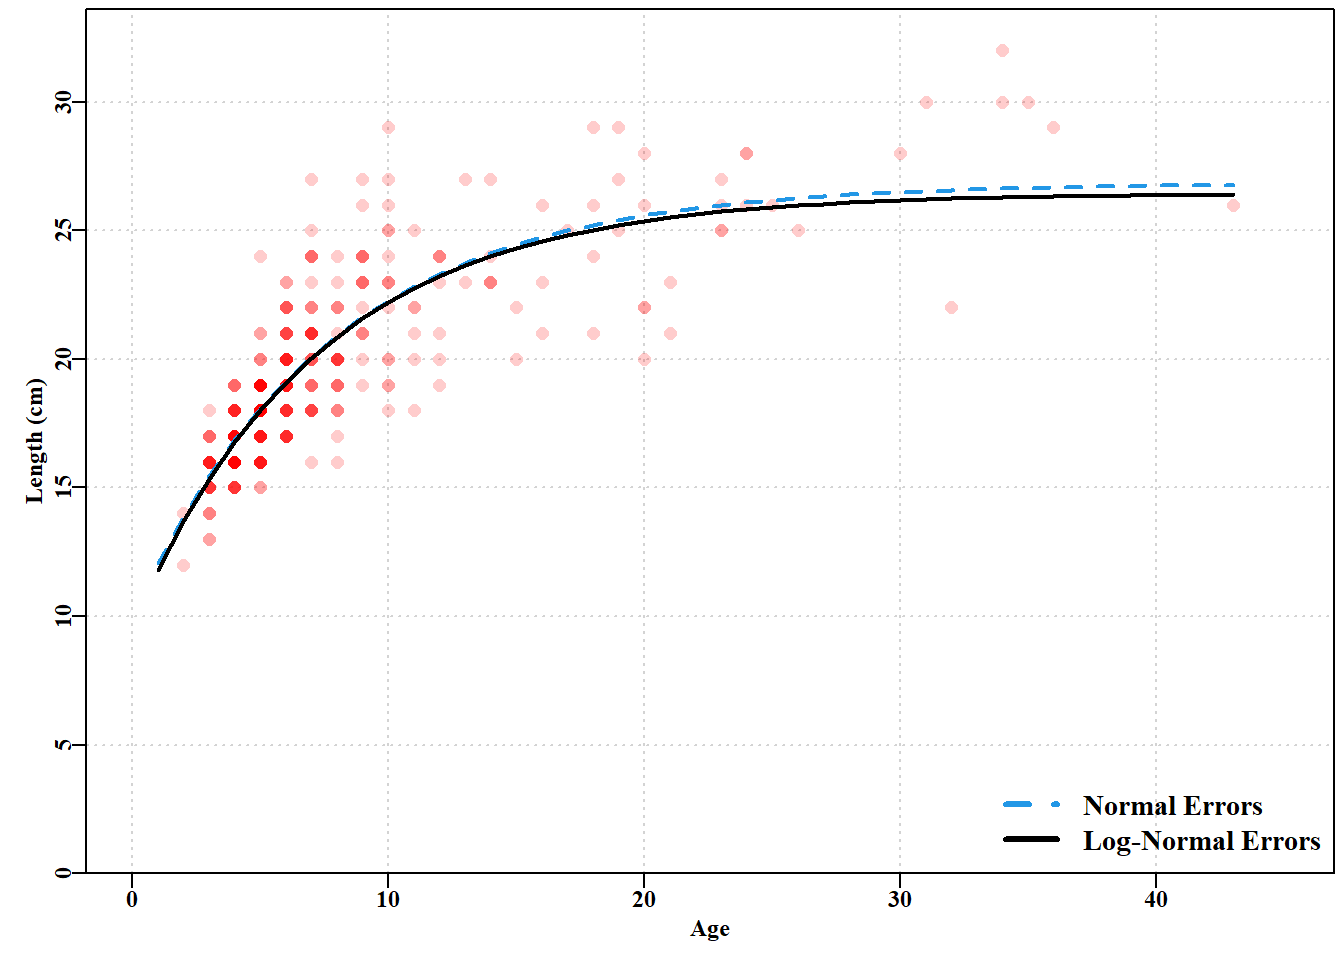
\includegraphics[keepaspectratio]{04-application_files/figure-latex/fig44-1.pdf}}
\caption{\label{fig:fig44}Female Length-at-Age data from 358 female redfish, Centroberyx affinis, with two von Bertalanffy growth curves fitted using Normal and Log-Normal residuals.}
\end{figure}

\subsection{关于初始模型拟合的说明}\label{ux5173ux4e8eux521dux59cbux6a21ux578bux62dfux5408ux7684ux8bf4ux660e}

上面例子中的曲线比较本身就很有趣,不过,我们还说明了 \texttt{nlm()} 的语法以及如何将模型拟合到数据中。将函数作为参数传递给另一个函数的能力(就像这里我们将 \texttt{ssq} 作为 \emph{f} 传递给 \texttt{nlm()},将 \texttt{vB}、\texttt{Gz} 和 \texttt{mm} 作为 \emph{funk} 传递给 \texttt{ssq()})是 R 的优势之一,但也是其复杂性所在。它简化了\texttt{ssq()}等函数的重用,在这些函数中,我们只需改变输入函数,就能从本质上相同的代码中得到完全不同的答案。熟悉这些方法的最佳途径是使用自己的数据集。绘制您的数据和任何模型拟合图,因为如果模型拟合图看起来不寻常,那么很可能就是不寻常的,值得再看一遍或三遍。

使用平方和法可以取得很好的效果,但在处理现实世界的多样性时,要求在期望值附近的残差呈正态分布以及方差恒定的假设是有限制的。为了使用正态分布以外的概率密度分布和非恒定方差,我们应该转而使用最大似然法。

\section{最大似然}\label{ux6700ux5927ux4f3cux7136}

在 R 中使用似然比较简单,因为有许多概率密度函数(PDF)的内置函数以及一系列定义其他 PDF 的软件包。再重复一遍,最大似然法的目的是使用软件搜索模型参数集,使观测数据的总似然最大化。要使用这一最优模型拟合标准,需要对模型进行定义,以便将每个观测值(可用数据)的概率或似然值指定为模型中参数值和其他变量的函数(式\eqref{eq:eq42}和式\eqref{eq:eq411})。重要的是,这种规范包括对所选 PDF 的变异性或扩散性的估计(正态分布中的\(\sigma\) 只是最小二乘法的副产品)。使用最大似然法的一个主要优点是,残差结构或关于数据预期中心倾向的观测值的预期分布不一定是正态分布。如果可以定义概率密度函数 (PDF),则可以在最大似然法框架中使用;有关许多有用概率密度函数的定义,请参见 Forbes et al, (2011)。

\subsection{入门范例}\label{ux5165ux95e8ux8303ux4f8b}

我们将使用众所周知的正态分布来说明这些方法,然后扩展该方法以包含一系列可选的pdf。对于数据模型拟合而言,每个PDF的主要意义在于定义单个观测值的概率密度或似然值。对于平均期望值为 \(\bar x\) 或 \(\mu\) 的正态分布,给定单一值 \(x_i\) 的概率密度或似然定义为:

\begin{equation}  
L\left( {x_i}|\mu_{i} ,\sigma  \right)=\frac{1}{\sigma \sqrt{2\pi }}{{e}^{\left( \frac{-{{\left( {x_i}-\mu_{i}  \right)}^{2}}}{2\sigma^2 } \right)}}  
\label{eq:eq411}  
\end{equation}

其中\(\sigma\) 为与\(\mu_i\) 相关的标准差。这确定了最小二乘法和最大似然方法之间的直接区别,在后者中,需要一个PDF的完整定义,在正态分布的情况下,它包括对均值估计 \(\mu\) 周围残差的标准偏差的显式估计。这样的估计不需要最小二乘,虽然很容易从SSQ值中得到。

例如,我们可以从正态分布中生成一个观测样本(参见\texttt{?rnorm}),然后计算该样本的均值和标准差,并比较给定的样本值与 \emph{rnorm} 函数中使用的原始均值和标准差的参数估计值的可能性有多大(表\ref{tab:tab41} ):

\begin{Shaded}
\begin{Highlighting}[]
 \CommentTok{\# Illustrate Normal random likelihoods. see Table 4.1  }
\FunctionTok{set.seed}\NormalTok{(}\DecValTok{12345}\NormalTok{)       }\CommentTok{\# make the use of random numbers repeatable  }
\NormalTok{x }\OtherTok{\textless{}{-}} \FunctionTok{rnorm}\NormalTok{(}\DecValTok{10}\NormalTok{,}\AttributeTok{mean=}\FloatTok{5.0}\NormalTok{,}\AttributeTok{sd=}\FloatTok{1.0}\NormalTok{)      }\CommentTok{\# pseudo{-}randomly generate 10   }
\NormalTok{avx }\OtherTok{\textless{}{-}} \FunctionTok{mean}\NormalTok{(x)                      }\CommentTok{\# normally distributed values  }
\NormalTok{sdx }\OtherTok{\textless{}{-}} \FunctionTok{sd}\NormalTok{(x)          }\CommentTok{\# estimate the mean and stdev of the sample            }
\NormalTok{L1 }\OtherTok{\textless{}{-}} \FunctionTok{dnorm}\NormalTok{(x,}\AttributeTok{mean=}\FloatTok{5.0}\NormalTok{,}\AttributeTok{sd=}\FloatTok{1.0}\NormalTok{)   }\CommentTok{\# obtain likelihoods, L1, L2 for   }
\NormalTok{L2 }\OtherTok{\textless{}{-}} \FunctionTok{dnorm}\NormalTok{(x,}\AttributeTok{mean=}\NormalTok{avx,}\AttributeTok{sd=}\NormalTok{sdx)    }\CommentTok{\# each data point for both sets  }
\NormalTok{result }\OtherTok{\textless{}{-}} \FunctionTok{cbind}\NormalTok{(x,L1,L2,}\StringTok{"L2gtL1"}\OtherTok{=}\NormalTok{(L2}\SpecialCharTok{\textgreater{}}\NormalTok{L1))      }\CommentTok{\# which is larger?  }
\NormalTok{result }\OtherTok{\textless{}{-}} \FunctionTok{rbind}\NormalTok{(result,}\FunctionTok{c}\NormalTok{(}\ConstantTok{NA}\NormalTok{,}\FunctionTok{prod}\NormalTok{(L1),}\FunctionTok{prod}\NormalTok{(L2),}\DecValTok{1}\NormalTok{)) }\CommentTok{\# result+totals  }
\FunctionTok{rownames}\NormalTok{(result) }\OtherTok{\textless{}{-}} \FunctionTok{c}\NormalTok{(}\DecValTok{1}\SpecialCharTok{:}\DecValTok{10}\NormalTok{,}\StringTok{"product"}\NormalTok{)  }
\FunctionTok{colnames}\NormalTok{(result) }\OtherTok{\textless{}{-}} \FunctionTok{c}\NormalTok{(}\StringTok{"x"}\NormalTok{,}\StringTok{"original"}\NormalTok{,}\StringTok{"estimated"}\NormalTok{,}\StringTok{"est \textgreater{} orig"}\NormalTok{)  }
\NormalTok{knitr}\SpecialCharTok{::}\FunctionTok{kable}\NormalTok{(result, }\AttributeTok{caption =} \StringTok{"An illustration of using normal random values and related normal likelihoods. The estimated column has the larger total likelihood. 1=TRUE, 0=FALSE."}\NormalTok{)}
\end{Highlighting}
\end{Shaded}

\begin{longtable}[]{@{}lrrrr@{}}
\caption{\label{tab:tab41}An illustration of using normal random values and related normal likelihoods. The estimated column has the larger total likelihood. 1=TRUE, 0=FALSE.}\tabularnewline
\toprule\noalign{}
& x & original & estimated & est \textgreater{} orig \\
\midrule\noalign{}
\endfirsthead
\toprule\noalign{}
& x & original & estimated & est \textgreater{} orig \\
\midrule\noalign{}
\endhead
\bottomrule\noalign{}
\endlastfoot
1 & 5.585529 & 0.3360953 & 0.3320130 & 0 \\
2 & 5.709466 & 0.3101778 & 0.2868818 & 0 \\
3 & 4.890697 & 0.3965663 & 0.4901017 & 1 \\
4 & 4.546503 & 0.3599578 & 0.4536973 & 1 \\
5 & 5.605887 & 0.3320438 & 0.3246562 & 0 \\
6 & 3.182044 & 0.0764269 & 0.0574370 & 0 \\
7 & 5.630099 & 0.3271127 & 0.3158617 & 0 \\
8 & 4.723816 & 0.3840136 & 0.4827694 & 1 \\
9 & 4.715840 & 0.3831564 & 0.4819139 & 1 \\
10 & 4.080678 & 0.2614493 & 0.3073533 & 1 \\
product & NA & 0.0000048 & 0.0000089 & 1 \\
\end{longtable}

表\ref{tab:tab41}的最下面一行包含每列似然值的乘积(使用R函数\texttt{prod()}求得)。毫不奇怪,当我们使用样本的均值和标准差估计(估计,L2)而不是原始值的\emph{mean=5}和\emph{sd=1.0}(原始,L1)时,求得最大似然,即8.9201095\^{}\{-6\} \textgreater{} 4.7521457 \^{}\{6\}。在本例中,我可以确定这些值,因为在代码开始时使用了R函数\texttt{set.seed()} ,以便在特定位置启动伪随机数生成器。如果你通常使用\texttt{set.seed()},不会重复使用相同的旧序列,例如12345,因为您可能会破坏伪随机数是随机数序列的良好近似值的想法,也许可以使用\texttt{getseed()}来提供合适的种子数。

因此,\texttt{rnorm()} 函数提供了由均值和 stdev 确定分布中的伪随机数,\texttt{dnorm()} 函数提供了观测值在均值和 stdev 条件下的概率密度或似然(相当于式\eqref{eq:eq411})。累积概率密度函数(cdf)由函数 \texttt{pnorm()} 提供,量化值由 \texttt{qnorm()} 确定。平均值自然具有最大的似然。还要注意的是,正态曲线是围绕均值对称的。

\begin{Shaded}
\begin{Highlighting}[]
 \CommentTok{\# some examples of pnorm, dnorm, and qnorm, all mean = 0  }
\FunctionTok{cat}\NormalTok{(}\StringTok{"x = 0.0        Likelihood ="}\NormalTok{,}\FunctionTok{dnorm}\NormalTok{(}\FloatTok{0.0}\NormalTok{,}\AttributeTok{mean=}\DecValTok{0}\NormalTok{,}\AttributeTok{sd=}\DecValTok{1}\NormalTok{),}\StringTok{"}\SpecialCharTok{\textbackslash{}n}\StringTok{"}\NormalTok{)   }
\end{Highlighting}
\end{Shaded}

\begin{verbatim}
## x = 0.0        Likelihood = 0.3989423
\end{verbatim}

\begin{Shaded}
\begin{Highlighting}[]
\FunctionTok{cat}\NormalTok{(}\StringTok{"x = 1.95996395 Likelihood ="}\NormalTok{,}\FunctionTok{dnorm}\NormalTok{(}\FloatTok{1.95996395}\NormalTok{,}\AttributeTok{mean=}\DecValTok{0}\NormalTok{,}\AttributeTok{sd=}\DecValTok{1}\NormalTok{),}\StringTok{"}\SpecialCharTok{\textbackslash{}n}\StringTok{"}\NormalTok{)   }
\end{Highlighting}
\end{Shaded}

\begin{verbatim}
## x = 1.95996395 Likelihood = 0.05844507
\end{verbatim}

\begin{Shaded}
\begin{Highlighting}[]
\FunctionTok{cat}\NormalTok{(}\StringTok{"x ={-}1.95996395 Likelihood ="}\NormalTok{,}\FunctionTok{dnorm}\NormalTok{(}\SpecialCharTok{{-}}\FloatTok{1.95996395}\NormalTok{,}\AttributeTok{mean=}\DecValTok{0}\NormalTok{,}\AttributeTok{sd=}\DecValTok{1}\NormalTok{),}\StringTok{"}\SpecialCharTok{\textbackslash{}n}\StringTok{"}\NormalTok{)   }
\end{Highlighting}
\end{Shaded}

\begin{verbatim}
## x =-1.95996395 Likelihood = 0.05844507
\end{verbatim}

\begin{Shaded}
\begin{Highlighting}[]
 \CommentTok{\# 0.5 = half cumulative distribution  }
\FunctionTok{cat}\NormalTok{(}\StringTok{"x = 0.0        cdf = "}\NormalTok{,}\FunctionTok{pnorm}\NormalTok{(}\DecValTok{0}\NormalTok{,}\AttributeTok{mean=}\DecValTok{0}\NormalTok{,}\AttributeTok{sd=}\DecValTok{1}\NormalTok{),}\StringTok{"}\SpecialCharTok{\textbackslash{}n}\StringTok{"}\NormalTok{)   }
\end{Highlighting}
\end{Shaded}

\begin{verbatim}
## x = 0.0        cdf =  0.5
\end{verbatim}

\begin{Shaded}
\begin{Highlighting}[]
\FunctionTok{cat}\NormalTok{(}\StringTok{"x = 0.6744899  cdf = "}\NormalTok{,}\FunctionTok{pnorm}\NormalTok{(}\FloatTok{0.6744899}\NormalTok{,}\AttributeTok{mean=}\DecValTok{0}\NormalTok{,}\AttributeTok{sd=}\DecValTok{1}\NormalTok{),}\StringTok{"}\SpecialCharTok{\textbackslash{}n}\StringTok{"}\NormalTok{)  }
\end{Highlighting}
\end{Shaded}

\begin{verbatim}
## x = 0.6744899  cdf =  0.75
\end{verbatim}

\begin{Shaded}
\begin{Highlighting}[]
\FunctionTok{cat}\NormalTok{(}\StringTok{"x = 0.75       Quantile ="}\NormalTok{,}\FunctionTok{qnorm}\NormalTok{(}\FloatTok{0.75}\NormalTok{),}\StringTok{"}\SpecialCharTok{\textbackslash{}n}\StringTok{"}\NormalTok{) }\CommentTok{\# reverse pnorm  }
\end{Highlighting}
\end{Shaded}

\begin{verbatim}
## x = 0.75       Quantile = 0.6744898
\end{verbatim}

\begin{Shaded}
\begin{Highlighting}[]
\FunctionTok{cat}\NormalTok{(}\StringTok{"x = 1.95996395 cdf = "}\NormalTok{,}\FunctionTok{pnorm}\NormalTok{(}\FloatTok{1.95996395}\NormalTok{,}\AttributeTok{mean=}\DecValTok{0}\NormalTok{,}\AttributeTok{sd=}\DecValTok{1}\NormalTok{),}\StringTok{"}\SpecialCharTok{\textbackslash{}n}\StringTok{"}\NormalTok{)  }
\end{Highlighting}
\end{Shaded}

\begin{verbatim}
## x = 1.95996395 cdf =  0.975
\end{verbatim}

\begin{Shaded}
\begin{Highlighting}[]
\FunctionTok{cat}\NormalTok{(}\StringTok{"x ={-}1.95996395 cdf = "}\NormalTok{,}\FunctionTok{pnorm}\NormalTok{(}\SpecialCharTok{{-}}\FloatTok{1.95996395}\NormalTok{,}\AttributeTok{mean=}\DecValTok{0}\NormalTok{,}\AttributeTok{sd=}\DecValTok{1}\NormalTok{),}\StringTok{"}\SpecialCharTok{\textbackslash{}n}\StringTok{"}\NormalTok{)  }
\end{Highlighting}
\end{Shaded}

\begin{verbatim}
## x =-1.95996395 cdf =  0.025
\end{verbatim}

\begin{Shaded}
\begin{Highlighting}[]
\FunctionTok{cat}\NormalTok{(}\StringTok{"x = 0.975      Quantile ="}\NormalTok{,}\FunctionTok{qnorm}\NormalTok{(}\FloatTok{0.975}\NormalTok{),}\StringTok{"}\SpecialCharTok{\textbackslash{}n}\StringTok{"}\NormalTok{) }\CommentTok{\# expect \textasciitilde{}1.96  }
\end{Highlighting}
\end{Shaded}

\begin{verbatim}
## x = 0.975      Quantile = 1.959964
\end{verbatim}

\begin{Shaded}
\begin{Highlighting}[]
 \CommentTok{\# try x \textless{}{-} seq({-}5,5,0.2); round(dnorm(x,mean=0.0,sd=1.0),5)  }
\end{Highlighting}
\end{Shaded}

我们可以看到,单个似然值可能是相对较大的数字,但当它们相乘时,很快就会变成相对较小的数字。当观测数据的数量增加时,就会出现误差。即使只有十个数字,当我们将所有单个似然值相乘(使用 \texttt{prod()})时,结果也会很快变得非常小。如果使用与表\ref{tab:tab41}中的十个数字类似的另外十个数字,总似然很容易降到 1e-11 或 1e-12。随着观察次数的增加,出现四舍五入错误的几率(即使在 64 位计算机上)也开始增加。与其将许多小数相乘得到一个极小的数,不如将这些小数相乘的标准解决方案是对似然值进行自然对数变换,然后相加。最大化对数变换似然值之和与最大化单个似然值之积一样,都能获得最佳参数。此外,许多软件中的优化器似乎都是为了最有效地最小化某个函数而设计的。简单的解决方案是,我们不最大化单个似然的乘积,而是最小化负对数似然的总和(\emph{-veLL} 或 \texttt{negLL()})。

\section{正态分布的似然}\label{ux6b63ux6001ux5206ux5e03ux7684ux4f3cux7136}

概率似乎是一种相当奇怪的生物。当它们来自连续的概率密度函数(PDFs)时,尽管它们具有许多相同的属性,但严格来说它们并不是概率(Edwards,1972 )。严格来讲,它们与概率密度函数下某一点的概率密度有关。根据概率的定义,整条曲线下的面积总和必须为 1.0,但连续概率密度函数任何一点下的面积都会变得无穷小。正态似然的定义使用式\eqref{eq:eq411}),而累积密度函数为:

\begin{equation}  
{cdf}=1=\int\limits_{x=-\infty }^{\infty }{\frac{1}{\sigma \sqrt{2\pi }}}{{e}^{\left( \frac{-{{\left( x-\mu  \right)}^{2}}}{2{{\sigma }^{2}}} \right)}}  
\label{eq:eq412}  
\end{equation}

我们可以使用\texttt{dnorm()} 和 \texttt{pnorm()} 计算似然和累积密度函数(cdf)(图\ref{fig:fig45})。

\begin{Shaded}
\begin{Highlighting}[]
 \CommentTok{\# Density plot and cumulative distribution for Normal   Fig 4.5  }
\NormalTok{x }\OtherTok{\textless{}{-}} \FunctionTok{seq}\NormalTok{(}\SpecialCharTok{{-}}\DecValTok{5}\NormalTok{,}\DecValTok{5}\NormalTok{,}\FloatTok{0.1}\NormalTok{)  }\CommentTok{\# a sequence of values around a mean of 0.0  }
\NormalTok{NL }\OtherTok{\textless{}{-}} \FunctionTok{dnorm}\NormalTok{(x,}\AttributeTok{mean=}\DecValTok{0}\NormalTok{,}\AttributeTok{sd=}\FloatTok{1.0}\NormalTok{)   }\CommentTok{\# normal likelihoods for each X  }
\NormalTok{CD }\OtherTok{\textless{}{-}} \FunctionTok{pnorm}\NormalTok{(x,}\AttributeTok{mean=}\DecValTok{0}\NormalTok{,}\AttributeTok{sd=}\FloatTok{1.0}\NormalTok{)   }\CommentTok{\# cumulative density vs X  }
\FunctionTok{plot1}\NormalTok{(x,CD,}\AttributeTok{xlab=}\StringTok{"x = StDev from Mean"}\NormalTok{,}\AttributeTok{ylab=}\StringTok{"Likelihood and CDF"}\NormalTok{)  }
\FunctionTok{lines}\NormalTok{(x,NL,}\AttributeTok{lwd=}\DecValTok{3}\NormalTok{,}\AttributeTok{col=}\DecValTok{2}\NormalTok{,}\AttributeTok{lty=}\DecValTok{3}\NormalTok{) }\CommentTok{\# dashed line as these are points  }
\FunctionTok{abline}\NormalTok{(}\AttributeTok{h=}\FloatTok{0.5}\NormalTok{,}\AttributeTok{col=}\DecValTok{4}\NormalTok{,}\AttributeTok{lwd=}\DecValTok{1}\NormalTok{)  }
\end{Highlighting}
\end{Shaded}

\begin{figure}
\centering
\pandocbounded{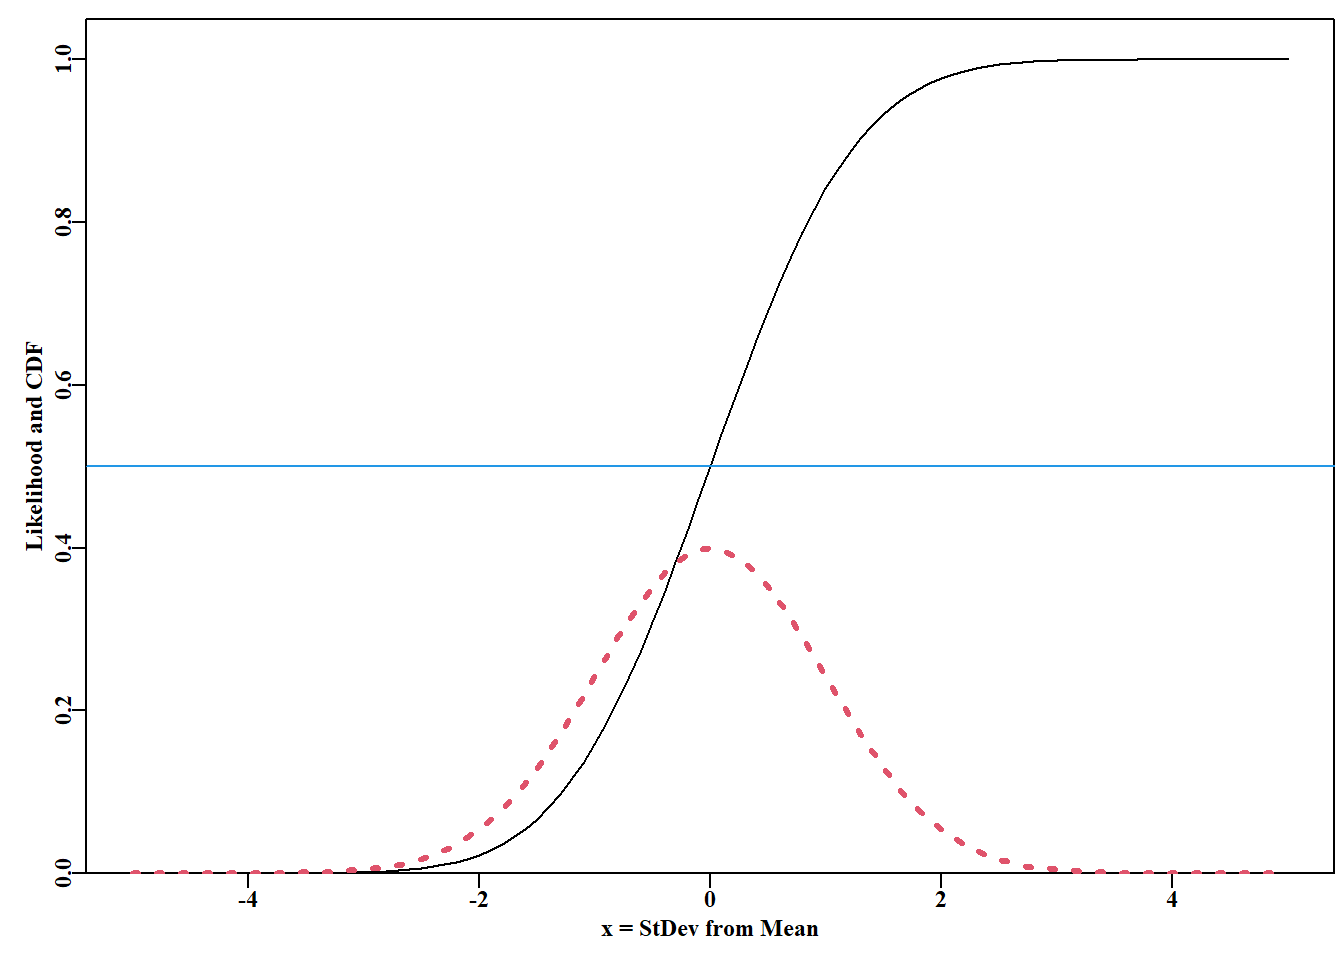
\includegraphics[keepaspectratio]{04-application_files/figure-latex/fig45-1.pdf}}
\caption{\label{fig:fig45}A dotted red curve depicting the expected normal likelihoods for a mean = 0 and sd = 1.0, along with the cumulative density of the same normal likelihoods as a black line. The blue line identifies a cumulative probability of 0.5.}
\end{figure}

这听起来不错,但在这样的曲线下,\emph{x}变量的特定值来说,确定这样一条曲线下的特定值意味着什么呢?在图\ref{fig:fig45}中,我们用虚线表示图中的似然是局部估计,不构成连续的线。每个都表示在给定\emph{x}值处的似然。我们在上文中已经看到,对于mean= 0.0和stdev = 1.0的分布,在0.0值处的概率密度为0.3989423。让我们简单地查看一下似然和概率之间可能存在的混淆。如果我们考虑概率密度函数的一小部分,在x = 3.4到3.6的值之间mean= 5.0,st.dev = 1.0的概率密度函数,我们可能会看到类似图\ref{fig:fig46}的情况:

\begin{Shaded}
\begin{Highlighting}[]
 \CommentTok{\#function facilitates exploring different polygons Fig 4.6  }
\NormalTok{plotpoly }\OtherTok{\textless{}{-}} \ControlFlowTok{function}\NormalTok{(mid,delta,}\AttributeTok{av=}\FloatTok{5.0}\NormalTok{,}\AttributeTok{stdev=}\FloatTok{1.0}\NormalTok{) \{  }
\NormalTok{   neg }\OtherTok{\textless{}{-}}\NormalTok{ mid}\SpecialCharTok{{-}}\NormalTok{delta;  pos }\OtherTok{\textless{}{-}}\NormalTok{ mid}\SpecialCharTok{+}\NormalTok{delta  }
\NormalTok{   pdval }\OtherTok{\textless{}{-}} \FunctionTok{dnorm}\NormalTok{(}\FunctionTok{c}\NormalTok{(mid,neg,pos),}\AttributeTok{mean=}\NormalTok{av,}\AttributeTok{sd=}\NormalTok{stdev)  }
   \FunctionTok{polygon}\NormalTok{(}\FunctionTok{c}\NormalTok{(neg,neg,mid,neg),}\FunctionTok{c}\NormalTok{(pdval[}\DecValTok{2}\NormalTok{],pdval[}\DecValTok{1}\NormalTok{],pdval[}\DecValTok{1}\NormalTok{],  }
\NormalTok{                          pdval[}\DecValTok{2}\NormalTok{]),}\AttributeTok{col=}\FunctionTok{rgb}\NormalTok{(}\FloatTok{0.25}\NormalTok{,}\FloatTok{0.25}\NormalTok{,}\FloatTok{0.25}\NormalTok{,}\FloatTok{0.5}\NormalTok{))  }
   \FunctionTok{polygon}\NormalTok{(}\FunctionTok{c}\NormalTok{(pos,pos,mid,pos),}\FunctionTok{c}\NormalTok{(pdval[}\DecValTok{1}\NormalTok{],pdval[}\DecValTok{3}\NormalTok{],pdval[}\DecValTok{1}\NormalTok{],  }
\NormalTok{                                pdval[}\DecValTok{1}\NormalTok{]),}\AttributeTok{col=}\FunctionTok{rgb}\NormalTok{(}\DecValTok{0}\NormalTok{,}\DecValTok{1}\NormalTok{,}\DecValTok{0}\NormalTok{,}\FloatTok{0.5}\NormalTok{))     }
   \FunctionTok{polygon}\NormalTok{(}\FunctionTok{c}\NormalTok{(mid,neg,neg,mid,mid),  }
        \FunctionTok{c}\NormalTok{(}\DecValTok{0}\NormalTok{,}\DecValTok{0}\NormalTok{,pdval[}\DecValTok{1}\NormalTok{],pdval[}\DecValTok{1}\NormalTok{],}\DecValTok{0}\NormalTok{),}\AttributeTok{lwd=}\DecValTok{2}\NormalTok{,}\AttributeTok{lty=}\DecValTok{1}\NormalTok{,}\AttributeTok{border=}\DecValTok{2}\NormalTok{)  }
   \FunctionTok{polygon}\NormalTok{(}\FunctionTok{c}\NormalTok{(mid,pos,pos,mid,mid),  }
        \FunctionTok{c}\NormalTok{(}\DecValTok{0}\NormalTok{,}\DecValTok{0}\NormalTok{,pdval[}\DecValTok{1}\NormalTok{],pdval[}\DecValTok{1}\NormalTok{],}\DecValTok{0}\NormalTok{),}\AttributeTok{lwd=}\DecValTok{2}\NormalTok{,}\AttributeTok{lty=}\DecValTok{1}\NormalTok{,}\AttributeTok{border=}\DecValTok{2}\NormalTok{)   }
   \FunctionTok{text}\NormalTok{(}\FloatTok{3.395}\NormalTok{,}\FloatTok{0.025}\NormalTok{,}\FunctionTok{paste0}\NormalTok{(}\StringTok{"\textasciitilde{}"}\NormalTok{,}\FunctionTok{round}\NormalTok{((}\DecValTok{2}\SpecialCharTok{*}\NormalTok{(delta}\SpecialCharTok{*}\NormalTok{pdval[}\DecValTok{1}\NormalTok{])),}\DecValTok{7}\NormalTok{)),}
        \AttributeTok{cex=}\FloatTok{1.1}\NormalTok{,}\AttributeTok{pos=}\DecValTok{4}\NormalTok{)  }
   \FunctionTok{return}\NormalTok{(}\DecValTok{2}\SpecialCharTok{*}\NormalTok{(delta}\SpecialCharTok{*}\NormalTok{pdval[}\DecValTok{1}\NormalTok{])) }\CommentTok{\# approx probability, see below  }
\NormalTok{\} }\CommentTok{\# end of plotpoly, a temporary function to enable flexibility  }
 \CommentTok{\#This code can be re{-}run with different values for delta  }
\NormalTok{x }\OtherTok{\textless{}{-}} \FunctionTok{seq}\NormalTok{(}\FloatTok{3.4}\NormalTok{,}\FloatTok{3.6}\NormalTok{,}\FloatTok{0.05}\NormalTok{) }\CommentTok{\# where under the normal curve to examine  }
\NormalTok{pd }\OtherTok{\textless{}{-}} \FunctionTok{dnorm}\NormalTok{(x,}\AttributeTok{mean=}\FloatTok{5.0}\NormalTok{,}\AttributeTok{sd=}\FloatTok{1.0}\NormalTok{) }\CommentTok{\#prob density for each X value  }
\NormalTok{mid }\OtherTok{\textless{}{-}} \FunctionTok{mean}\NormalTok{(x)      }
\NormalTok{delta }\OtherTok{\textless{}{-}} \FloatTok{0.05}  \CommentTok{\# how wide either side of the sample mean to go?   }
\FunctionTok{parset}\NormalTok{()       }\CommentTok{\# a pre{-}defined MQMF base graphics set{-}up for par  }
\NormalTok{ymax }\OtherTok{\textless{}{-}} \FunctionTok{getmax}\NormalTok{(pd)    }\CommentTok{\# find maximum y value for the plot  }
\FunctionTok{plot}\NormalTok{(x,pd,}\AttributeTok{type=}\StringTok{"l"}\NormalTok{,}\AttributeTok{xlab=}\StringTok{"Variable x"}\NormalTok{,}\AttributeTok{ylab=}\StringTok{"Probability Density"}\NormalTok{,  }
     \AttributeTok{ylim=}\FunctionTok{c}\NormalTok{(}\DecValTok{0}\NormalTok{,ymax),}\AttributeTok{yaxs=}\StringTok{"i"}\NormalTok{,}\AttributeTok{lwd=}\DecValTok{2}\NormalTok{,}\AttributeTok{panel.first=}\FunctionTok{grid}\NormalTok{())  }
\NormalTok{approxprob }\OtherTok{\textless{}{-}} \FunctionTok{plotpoly}\NormalTok{(mid,delta)  }\CommentTok{\#use function defined above  }
\end{Highlighting}
\end{Shaded}

\begin{figure}
\centering
\pandocbounded{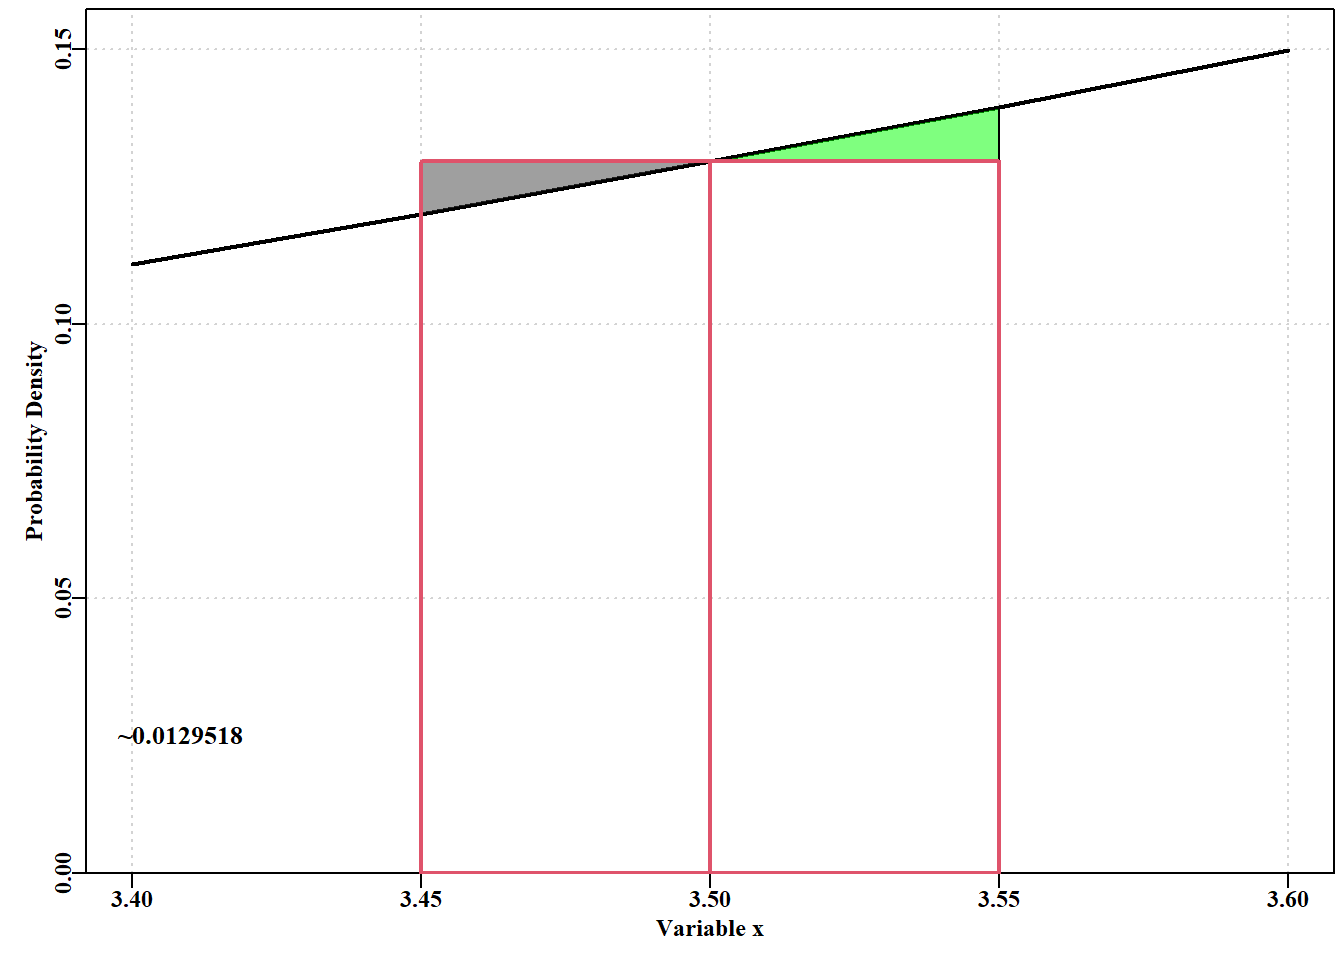
\includegraphics[keepaspectratio]{04-application_files/figure-latex/fig46-1.pdf}}
\caption{\label{fig:fig46}Probability densities for a normally distributed variate X, with a mean of 5.0 and a standard deviation of 1.0. The PDF value at x = 3.5 is 0.129518, so the area of the boxes outlined in red is 0.0129518, which approximates the total probability of a value between 3.45 - 3.55, which would really be the area under the curve.}
\end{figure}

完整概率密度函数( PDF) 下的面积总和为 1.0,因此得到图\ref{fig:fig46}中 3.45 和 3.55 之间值的概率是长方形面积减去左三角形面积再加上右三角形面积之和。三角形几乎是对称的,因此可以近似地相互抵消,所以近似解法就是将其中一个长方形的面积乘以 2.0。当 delta(长方形在 x 轴上的宽度)为 0.05 时,概率 = 0.0129518。如果将 delta 值改为 0.01,那么近似概率 = 0.0025904,随着 delta 值的减小,总概率也随之减小,尽管 3.5 时的概率密度仍为 0.1295176。显然,似然值与连续 PDF 中的概率并不相同(见 Edwards, 1972)。曲线下面积概率的最佳估计值为 \texttt{pnorm(3.55,5,1)\ -\ pnorm(3.45,5,1)},即 = 0.0129585。

\subsection{与平方和等同}\label{ux4e0eux5e73ux65b9ux548cux7b49ux540c}

当使用正态似然来拟合数据模型时,我们实际做的是设置,使得每个可用观测值的负对数似然之和最小化。幸运的是,我们可以使用\texttt{dnorm()}来估计似然。事实上,如果我们使用正态分布残差或对数变换的对数正态分布数据使用极大似然方法拟合模型,则得到的参数估计与使用最小二乘法得到的参数估计相同(参见下文式\eqref{eq:eq419}的推导和形式)。拟合模型需要生成一组预测值\(\hat x\) (x-hat),为其他自变量\(\theta(x)\) 的函数,其中\(\theta\) 是函数关系中使用的参数列。n个观测值的对数似然定义为:

\begin{equation}  
LL(x|\theta)=\sum\limits_{i=1}^{n}{log\left( \frac{1}{\hat{\sigma }\sqrt{2\pi }}{{e}^{\left( \frac{-{{\left( {x_i}-{{\hat{x}}_{i}} \right)}^{2}}}{2{{{\hat{\sigma }}}^{2}}} \right)}} \right)}  
\label{eq:eq413}  
\end{equation}

\(LL(x|\theta)\) 读作给定\(\theta\) 个参数(\(\mu\) 和 \(\hat \sigma\))时观测值 \(x\) 的对数似然;符号''\textbar{}``读作''给定''。这个看似复杂的方程式其实可以大大简化。首先,我们可以将指数项之前的常数移到求和项之外,乘以\(n\) ,然后将剩余指数项的自然对数反变换为指数:

\begin{equation}  
LL(x|\theta)=n log\left( \frac{1}{\hat{\sigma }\sqrt{2\pi }} \right)+\frac{1}{2{\hat{\sigma }^{2}}}\sum\limits_{i=1}^{n}{\left( -{{\left( x_i-\hat{x}_i \right)}^{2}} \right)}  
\label{eq:eq414}  
\end{equation}

\(\hat \sigma^2\) 是数据方差的最大似然估计(记住是除以n而非n--1):

\begin{equation}  
{{\hat{\sigma }}^{2}}=\frac{\sum\limits_{i=1}^{n}{{{\left( x_i-\hat{x}_i \right)}^{2}}}}{n}  
\label{eq:eq415}  
\end{equation}

如果用式\eqref{eq:eq415}中 \(\hat \sigma^2\) 代入式\eqref{eq:eq414},则 \((x_i-\hat x_i)^2\) 用 \(-n/2\) 代替:

\begin{equation}  
LL(x|\theta)=n{log}\left( \left( {\hat{\sigma }\sqrt{2\pi }} \right)^{-1} \right) - \frac{n}{2}  
\label{eq:eq416}  
\end{equation}

化简平方根意味着将- 1移至对数项外面,n变成- n,我们可以将平方根变成指数1/2,然后将 \(\log(\hat \sigma)\) 项加到 \(\pi\) 项上:

\begin{equation}  
LL(x|\theta)=-n\left( {log}\left( {{\left( 2\pi  \right)}^{\frac{1}{2}}} \right)+{log}\left( {\hat{\sigma }} \right) \right)-\frac{n}{2}  
\label{eq:eq417}  
\end{equation}

将幂指数 \(1/2\) 移到第1个\emph{log}项外:

\begin{equation}  
LL(x|\theta)=-\frac{n}{2}\left( {log}\left( 2\pi  \right)+2{log}\left( {\hat{\sigma }} \right) \right)-\frac{n}{2}  
\label{eq:eq418}  
\end{equation}

然后将 \(n/2\) 简化,并将整个方程两边乘以- 1,以转换为负对数似然,从而得到正态分布值的负对数似然的最终简化:

\begin{equation}  
-LL(x|\theta)=\frac{n}{2}\left( {log}\left( 2\pi  \right) + 2{log} \left( {\hat{\sigma }} \right) + 1 \right)  
\label{eq:eq419}  
\end{equation}

其中唯一的非常数部分是 \(\hat \sigma\) 的值,它是残差平方和除以 n 的平方根,所以现在应该很清楚了,为什么使用最大似然时获得的参数,如果使用正态随机误差,与从最小二乘方法得到的参数相同。

\subsection{应用正态似然拟合数据模型}\label{ux5e94ux7528ux6b63ux6001ux4f3cux7136ux62dfux5408ux6570ux636eux6a21ux578b}

我们可以使用数据集 \emph{LatA} 中的模拟雌性红鱼数据重复这个例子,图,

我们可以使用数据集 LatA中的模拟雌性红鱼数据来重复这个例子(图 \ref{fig:fig47}),我们用它来说明平方残差之和的使用。理想情况下,我们应该得到相同的答案,但估计值为 \(\sigma\) 的估计值。\textbf{MQMF} 函数 \texttt{plot1()} 只是绘制单个图形(\emph{type=``l''}或 \emph{type=``p''};请参阅 \texttt{?plot1})的一种快速方法,没有太多空白。如果你比我更喜欢空白,请编辑 \texttt{plot1()}!

\begin{Shaded}
\begin{Highlighting}[]
 \CommentTok{\#plot of length{-}at{-}age data  Fig 4.7  }
\FunctionTok{data}\NormalTok{(LatA) }\CommentTok{\# load the redfish data set into memory and plot it  }
\NormalTok{ages }\OtherTok{\textless{}{-}}\NormalTok{ LatA}\SpecialCharTok{$}\NormalTok{age;  lengths }\OtherTok{\textless{}{-}}\NormalTok{ LatA}\SpecialCharTok{$}\NormalTok{length  }
\FunctionTok{plot1}\NormalTok{(ages,lengths,}\AttributeTok{xlab=}\StringTok{"Age"}\NormalTok{,}\AttributeTok{ylab=}\StringTok{"Length"}\NormalTok{,}\AttributeTok{type=}\StringTok{"p"}\NormalTok{,}\AttributeTok{cex=}\FloatTok{0.8}\NormalTok{,  }
      \AttributeTok{pch=}\DecValTok{16}\NormalTok{,}\AttributeTok{col=}\FunctionTok{rgb}\NormalTok{(}\DecValTok{1}\NormalTok{,}\DecValTok{0}\NormalTok{,}\DecValTok{0}\NormalTok{,}\DecValTok{1}\SpecialCharTok{/}\DecValTok{5}\NormalTok{))  }
\end{Highlighting}
\end{Shaded}

\begin{figure}
\centering
\pandocbounded{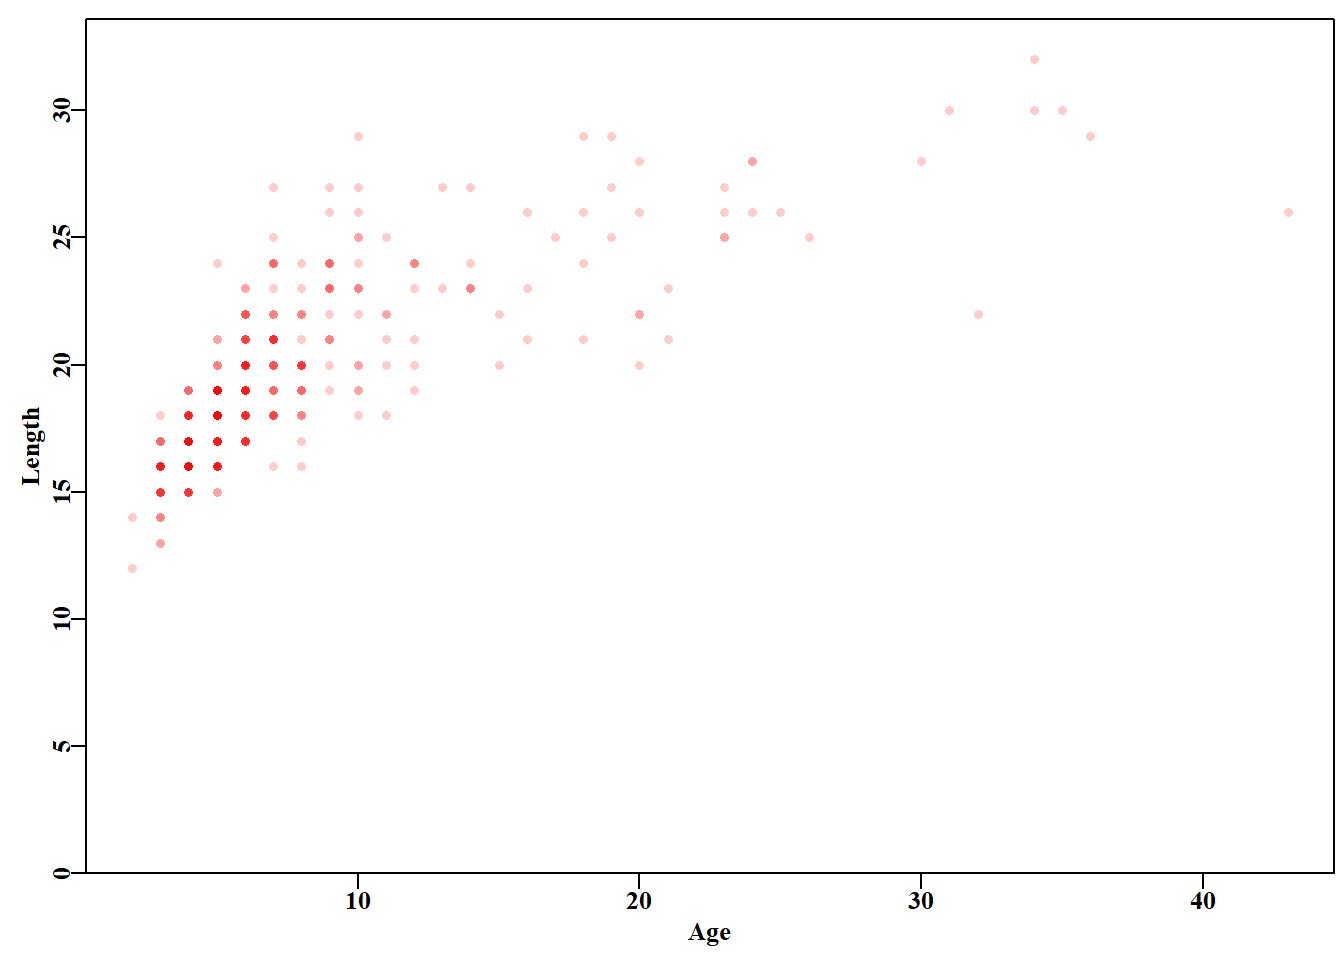
\includegraphics[keepaspectratio]{04-application_files/figure-latex/fig47-1.pdf}}
\caption{\label{fig:fig47}The length-at-age data contained within the LatA data set for female Redfish Centroberyx affinis. Full colour means \textgreater= 5 points.}
\end{figure}

现在,我们可以使用 \textbf{MQMF} 函数 \texttt{negNLL()}(负正态对数似然值)以确定使用正态随机误差的负对数似然值之和(\texttt{negLL()}对对数正态分布数据也有同样的作用)。如果你查看一下 \texttt{negNLL()} 的代码,就会发现它与 \texttt{ssq()} 一样,都是将一个函数作为参数传递给它,然后用它来计算每个输入年龄的预测平均值(在本例中是使用 \textbf{MQMF} 函数 \texttt{vB()}计算的年龄长度),然后使用 \texttt{dnorm()} 以预测值作为平均值,并使用数据中的年龄-长度观测值来计算 -veLL 之和。年龄数据是通过省略号(\ldots)传递的,并没有在 \texttt{negNLL()} 中明确声明为参数。该函数在结构上与 \texttt{ssq()} 非常相似,输入要求完全相同,但 \emph{pars} 是显式传递的,而不是在\ldots 中传递,因为 \emph{pars} 的最后一个值必须是残差的 stdev,它将在 \texttt{negNLL()} 中使用,而不只是在 \emph{funk} 中使用。因此,\texttt{negNLL()}的运行方式与\texttt{ssq()}非常相似,它是调用函数生成预测值的封装程序,然后使用 \texttt{dnorm()} 在每次调用时返回一个数字。因此,\texttt{nlm()} 会最小化 \texttt{negNLL()},而 \texttt{negNLL()} 又会调用 \texttt{vB()}。

\begin{Shaded}
\begin{Highlighting}[]
 \CommentTok{\# Fit the vB growth curve using maximum likelihood  }
\NormalTok{pars }\OtherTok{\textless{}{-}} \FunctionTok{c}\NormalTok{(}\AttributeTok{Linf=}\FloatTok{27.0}\NormalTok{,}\AttributeTok{K=}\FloatTok{0.15}\NormalTok{,}\AttributeTok{t0=}\SpecialCharTok{{-}}\FloatTok{3.0}\NormalTok{,}\AttributeTok{sigma=}\FloatTok{2.5}\NormalTok{) }\CommentTok{\# starting values  }
 \CommentTok{\# note, estimate for sigma is required for maximum likelihood  }
\NormalTok{ansvB }\OtherTok{\textless{}{-}} \FunctionTok{nlm}\NormalTok{(}\AttributeTok{f=}\NormalTok{negNLL,}\AttributeTok{p=}\NormalTok{pars,}\AttributeTok{funk=}\NormalTok{vB,}\AttributeTok{observed=}\NormalTok{lengths,}\AttributeTok{ages=}\NormalTok{ages,  }
             \AttributeTok{typsize=}\FunctionTok{magnitude}\NormalTok{(pars))  }
\end{Highlighting}
\end{Shaded}

\begin{verbatim}
## Warning in dnorm(x = observed, mean = predobs, sd = pars[npar], log
## = TRUE): NaNs produced
\end{verbatim}

\begin{verbatim}
## Warning in nlm(f = negNLL, p = pars, funk = vB, observed = lengths,
## ages = ages, : NA/Inf replaced by maximum positive value
\end{verbatim}

\begin{verbatim}
## Warning in dnorm(x = observed, mean = predobs, sd = pars[npar], log
## = TRUE): NaNs produced
\end{verbatim}

\begin{verbatim}
## Warning in nlm(f = negNLL, p = pars, funk = vB, observed = lengths,
## ages = ages, : NA/Inf replaced by maximum positive value
\end{verbatim}

\begin{Shaded}
\begin{Highlighting}[]
\FunctionTok{outfit}\NormalTok{(ansvB,}\AttributeTok{backtran=}\ConstantTok{FALSE}\NormalTok{,}\AttributeTok{title=}\StringTok{"vB by minimum {-}veLL"}\NormalTok{)  }
\end{Highlighting}
\end{Shaded}

\begin{verbatim}
## nlm solution:  vB by minimum -veLL 
## minimum     :  747.0795 
## iterations  :  26 
## code        :  1 gradient close to 0, probably solution 
##          par     gradient
## 1 26.8354474 4.448265e-07
## 2  0.1301554 1.659593e-05
## 3 -3.5868868 3.486464e-07
## 4  1.9500896 8.278354e-06
\end{verbatim}

\section{对数正态似然}\label{ux5bf9ux6570ux6b63ux6001ux4f3cux7136}

\chapter{Final Words}\label{final-words}

We have finished a nice book.

\appendix


\chapter{R Markdown}\label{r-markdown}

This is an R Markdown document. Markdown is a simple formatting syntax for authoring HTML, PDF, and MS Word documents. For more details on using R Markdown see \url{http://rmarkdown.rstudio.com}.

When you click the \textbf{Knit} button a document will be generated that includes both content as well as the output of any embedded R code chunks within the document. You can embed an R code chunk like this:

\begin{Shaded}
\begin{Highlighting}[]
\FunctionTok{summary}\NormalTok{(cars)}
\end{Highlighting}
\end{Shaded}

\begin{verbatim}
##      speed           dist       
##  Min.   : 4.0   Min.   :  2.00  
##  1st Qu.:12.0   1st Qu.: 26.00  
##  Median :15.0   Median : 36.00  
##  Mean   :15.4   Mean   : 42.98  
##  3rd Qu.:19.0   3rd Qu.: 56.00  
##  Max.   :25.0   Max.   :120.00
\end{verbatim}

\section{Including Plots}\label{including-plots}

You can also embed plots, for example:

\begin{Shaded}
\begin{Highlighting}[]
\FunctionTok{par}\NormalTok{(}\AttributeTok{mar =} \FunctionTok{c}\NormalTok{(}\DecValTok{4}\NormalTok{, }\DecValTok{4}\NormalTok{, .}\DecValTok{1}\NormalTok{, .}\DecValTok{1}\NormalTok{))}
\FunctionTok{plot}\NormalTok{(pressure)}
\end{Highlighting}
\end{Shaded}

\begin{figure}

{\centering \includegraphics[width=0.8\linewidth]{07-appendix_files/figure-latex/nice-fig-02-1} 

}

\caption{Here is another nice figure!}\label{fig:nice-fig-02}
\end{figure}

Note that the \texttt{echo\ =\ FALSE} parameter was added to the code chunk to prevent printing of the R code that generated the plot.

\chapter*{参考文献}\label{References}
\addcontentsline{toc}{chapter}{参考文献}

\phantomsection\label{refs}
\begin{CSLReferences}{1}{0}
\bibitem[\citeproctext]{ref-beverton1993a}
Beverton, Raymond J. H., and Sidney J. Holt. 1993. \emph{On the Dynamics of Exploited Fish Populations}. Springer Netherlands. \url{https://doi.org/10.1007/978-94-011-2106-4}.

\bibitem[\citeproctext]{ref-bickel1984}
Bickel, P. J., and D. A. Freedman. 1984. {``Asymptotic Normality and the Bootstrap in Stratified Sampling.''} \emph{The Annals of Statistics} 12 (2). \url{https://doi.org/10.1214/aos/1176346500}.

\bibitem[\citeproctext]{ref-birkes1993}
Birkes, David, and Yadolah Dodge. 1993. {``Alternative Methods of Regression.''} \emph{Wiley Series in Probability and Statistics}, June. \url{https://doi.org/10.1002/9781118150238}.

\bibitem[\citeproctext]{ref-modelse2004}
Burnham, Kenneth P., and David R. Anderson, eds. 2004. \emph{Model Selection and Multimodel Inference}. Springer New York. \url{https://doi.org/10.1007/b97636}.

\bibitem[\citeproctext]{ref-chambers2008}
Chambers, John M. 2008. \emph{Software for Data Analysis}. Springer New York. \url{https://doi.org/10.1007/978-0-387-75936-4}.

\bibitem[\citeproctext]{ref-chambers2017}
---------. 2017. \emph{Extending R}. Chapman; Hall/CRC. \url{https://doi.org/10.1201/9781315381305}.

\bibitem[\citeproctext]{ref-crawley2007}
Crawley, Michael J. 2007. {``The R Book,''} April. \url{https://doi.org/10.1002/9780470515075}.

\bibitem[\citeproctext]{ref-elder1979}
Elder, R. D. 1979. {``Equilibrium Yield for the Hauraki Gulf Snapper Fishery Estimated from Catch and Effort Figures, 1960{\textendash}74.''} \emph{New Zealand Journal of Marine and Freshwater Research} 13 (1): 31--38. \url{https://doi.org/10.1080/00288330.1979.9515778}.

\bibitem[\citeproctext]{ref-fournier1998}
Fournier, Daid A, John Hampton, and John R Sibert. 1998. {``MULTIFAN-CL: A Length-Based, Age-Structured Model for Fisheries Stock Assessment, with Application to South Pacific Albacore, {\emph{Thunnus Alalunga}}.''} \emph{Canadian Journal of Fisheries and Aquatic Sciences} 55 (9): 2105--16. \url{https://doi.org/10.1139/f98-100}.

\bibitem[\citeproctext]{ref-fournier2012}
Fournier, David A., Hans J. Skaug, Johnoel Ancheta, James Ianelli, Arni Magnusson, Mark N. Maunder, Anders Nielsen, and John Sibert. 2012. {``AD Model Builder: Using Automatic Differentiation for Statistical Inference of Highly Parameterized Complex Nonlinear Models.''} \emph{Optimization Methods and Software} 27 (2): 233--49. \url{https://doi.org/10.1080/10556788.2011.597854}.

\bibitem[\citeproctext]{ref-haddon2011}
Haddon, Malcolm. 2011. \emph{Modelling and Quantitative Methods in Fisheries}. Chapman; Hall/CRC. \url{https://doi.org/10.1201/9781439894170}.

\bibitem[\citeproctext]{ref-helidoniotis2013}
Helidoniotis, Fay, and Malcolm Haddon. 2013. {``Growth Models for Fisheries: The Effect of Unbalanced Sampling Error On Model Selection, Parameter Estimation, and Biological Predictions.''} \emph{Journal of Shellfish Research} 32 (1): 223--35. \url{https://doi.org/10.2983/035.032.0129}.

\bibitem[\citeproctext]{ref-hilborn1979}
Hilborn, Ray. 1979. {``Comparison of Fisheries Control Systems That Utilize Catch and Effort Data.''} \emph{Journal of the Fisheries Research Board of Canada} 36 (12): 1477--89. \url{https://doi.org/10.1139/f79-215}.

\bibitem[\citeproctext]{ref-hilborn1992}
Hilborn, Ray, and Carl J. Walters. 1992. \emph{Quantitative Fisheries Stock Assessment}. Springer US. \url{https://doi.org/10.1007/978-1-4615-3598-0}.

\bibitem[\citeproctext]{ref-iacobucci2012}
Iacobucci, Alessandra, and Christian Robert. 2012. {``The Art of R Programming: A Tour of Statistical Software Design by Norman Matloff.''} \emph{CHANCE} 25 (2): 55--56. \url{https://doi.org/10.1080/09332480.2012.685374}.

\bibitem[\citeproctext]{ref-kristensen2016}
Kristensen, Kasper, Anders Nielsen, Casper W. Berg, Hans Skaug, and Bradley M. Bell. 2016. {``{\textbf{TMB}}: Automatic Differentiation and Laplace Approximation.''} \emph{Journal of Statistical Software} 70 (5). \url{https://doi.org/10.18637/jss.v070.i05}.

\bibitem[\citeproctext]{ref-maccall2009}
MacCall, Alec D. 2009. {``Depletion-Corrected Average Catch: A Simple Formula for Estimating Sustainable Yields in Data-Poor Situations.''} \emph{ICES Journal of Marine Science} 66 (10): 2267--71. \url{https://doi.org/10.1093/icesjms/fsp209}.

\bibitem[\citeproctext]{ref-matloff2011}
Matloff, Norman. 2011. \emph{The Art of r Programming: A Tour of Statistical Software Design}. 1st edition. San Francisco: No Starch Press.

\bibitem[\citeproctext]{ref-theoreti2007}
May, Robert, and Angela R. McLean, eds. 2007. \emph{Theoretical Ecology}. Oxford University Press. \url{https://doi.org/10.1093/oso/9780199209989.001.0001}.

\bibitem[\citeproctext]{ref-murrell2018a}
Murrell, Paul. 2018. \emph{R Graphics, Third Edition}. Chapman; Hall/CRC. \url{https://doi.org/10.1201/9780429422768}.

\bibitem[\citeproctext]{ref-onthen}
{``On the Nature of the Function Expressive of the Law of Human Mortality and on a New Mode of Determining the Value of Life Contingencies: In a Letter to Francis Baily Esq. F.r.s. \&C., by Benjamin Gompertz ...''} n.d. Brill. \url{https://doi.org/10.1163/9789004460409_mor2-b29484479}.

\bibitem[\citeproctext]{ref-pitcher1973}
Pitcher, T. J., and P. D. M. Macdonald. 1973. {``Two Models for Seasonal Growth in Fishes.''} \emph{The Journal of Applied Ecology} 10 (2): 599. \url{https://doi.org/10.2307/2402304}.

\bibitem[\citeproctext]{ref-polacheck1993}
Polacheck, Tom, Ray Hilborn, and Andre E. Punt. 1993. {``Fitting Surplus Production Models: Comparing Methods and Measuring Uncertainty.''} \emph{Canadian Journal of Fisheries and Aquatic Sciences} 50 (12): 2597--607. \url{https://doi.org/10.1139/f93-284}.

\bibitem[\citeproctext]{ref-prager1994}
Prager, Michael. 1994. {``A Suite of Extensions to a Nonequilibrium Surplus-Production Model.''} \emph{Fishery Bulletin} 92 (January): 374--89.

\bibitem[\citeproctext]{ref-punt1997}
Punt, Andre E., and Ray Hilborn. 1997. {``Fisheries Stock Assessment and Decision Analysis: The Bayesian Approach.''} \emph{Reviews in Fish Biology and Fisheries} 7 (1): 35--63. \url{https://doi.org/10.1023/A:1018419207494}.

\bibitem[\citeproctext]{ref-quinn2003}
QUINN, TERRANCE J. 2003. {``RUMINATIONS ON THE DEVELOPMENT AND FUTURE OF POPULATION DYNAMICS MODELS IN FISHERIES.''} \emph{Natural Resource Modeling} 16 (4): 341--92. \url{https://doi.org/10.1111/j.1939-7445.2003.tb00119.x}.

\bibitem[\citeproctext]{ref-quinn1999}
Quinn, Terrance J., and Richard B. Deriso. 1999. \emph{Quantitative Fish Dynamics}. Biological Resource Management. Oxford, New York: Oxford University Press.

\bibitem[\citeproctext]{ref-russell1942}
Russell, E. S. 1942. \emph{The Overfishing Problem}. CUP Archive.

\bibitem[\citeproctext]{ref-saila1979}
Saila, S. B., J. H. Annala, J. L. McKoy, and J. D. Booth. 1979. {``Application of Yield Models to the New Zealand Rock Lobster Fishery.''} \emph{New Zealand Journal of Marine and Freshwater Research} 13 (1): 1--11. \url{https://doi.org/10.1080/00288330.1979.9515775}.

\bibitem[\citeproctext]{ref-schaefer1991}
Schaefer, M. 1991. {``Some Aspects of the Dynamics of Populations Important to the Management of the Commercial Marine Fisheries.''} \emph{Bulletin of Mathematical Biology} 53 (1-2): 253--79. \url{https://doi.org/10.1016/s0092-8240(05)80049-7}.

\bibitem[\citeproctext]{ref-schaefer1957}
Schaefer, M. B. 1957. {``A Study of the Dynamics of the Fishery for Yellowfin Tuna in the Eastern Tropical Pacific Ocean.''} In. \url{https://www.semanticscholar.org/paper/A-study-of-the-dynamics-of-the-fishery-for-tuna-in-Schaefer/29677d4a85d251d68d645584b2505c51c1ef1728}.

\bibitem[\citeproctext]{ref-stearns1992}
Stearns, SC. 1992. \emph{The Evolution of Life Histories}. Oxford University Press.

\bibitem[\citeproctext]{ref-stearns1977}
Stearns, Stephen C. 1977. {``The Evolution of Life History Traits: A Critique of the Theory and a Review of the Data.''} \emph{Annual Review of Ecology and Systematics} 8 (1): 145--71. \url{https://doi.org/10.1146/annurev.es.08.110177.001045}.

\bibitem[\citeproctext]{ref-venables2002}
Venables, W. N., and B. D. Ripley. 2002. \emph{Modern Applied Statistics with s}. Springer New York. \url{https://doi.org/10.1007/978-0-387-21706-2}.

\bibitem[\citeproctext]{ref-wickham2019}
Wickham, Hadley. 2019. \emph{Advanced R}. Chapman; Hall/CRC. \url{https://doi.org/10.1201/9781351201315}.

\bibitem[\citeproctext]{ref-winker2018}
Winker, Henning, Felipe Carvalho, and Maia Kapur. 2018. {``JABBA: Just Another Bayesian Biomass Assessment.''} \emph{Fisheries Research} 204 (August): 275--88. \url{https://doi.org/10.1016/j.fishres.2018.03.010}.

\bibitem[\citeproctext]{ref-xie2016a}
Xie, Yihui. 2016. {``Bookdown: Authoring Books and Technical Documents with r Markdown.''} The R Foundation. \url{https://doi.org/10.32614/cran.package.bookdown}.

\end{CSLReferences}

\end{document}
